\documentclass{article}
\usepackage{anyfontsize}
\usepackage[UTF8]{ctex} % 如果需要支持中文
\usepackage{fontspec} 
\setCJKmainfont{SourceHanSansCN-Light}[
    BoldFont=SourceHanSansCN-Medium
]

\usepackage[a4paper, left=0.1in, right=0.1in, top=0.05in, bottom=0.05in]{geometry} % 设置四边页边距为0.1英寸{geometry} % 设置页边距为0.5英寸
\usepackage{enumitem} % 用于自定义列表
\usepackage{amsmath}  % 数学公式支持

\setlength{\parindent}{0pt} % 不缩进
\usepackage{etoolbox} % 用于列表操作
%调整类代码
\usepackage{comment}
\usepackage{tocloft} % 用于定制目录样式
%\usepackage{hyperref} %不需要目录盒子注释这
\usepackage{ifthen}
\usepackage{tikz}
\usepackage{titletoc}
\usepackage{graphicx}
\usepackage{amssymb}  % 提供数学符号，包括\therefore
\usepackage{multirow} 
\usepackage{pgfplots}
\pgfplotsset{compat=1.15}
%目录设定
%快捷键 CMD + / 注释
%  \renewcommand{\cftdot}{} % 隐藏目录中的页码
%  \cftpagenumbersoff{section}
%  \cftpagenumbersoff{subsection}
%  \makeatletter
%  \renewcommand{\@pnumwidth}{0em}  % 设置页码宽度为0
%  \renewcommand{\@tocrmarg}{0em}   % 设置右边距为0
%  \makeatother
 


\usepackage{environ}

\newif\ifshowcontent  % 定义一个条件判断变量
\showcontenttrue    % 设置为 false，隐藏所有 question 环境的内容

\newcounter{question} % 题目计数器
\setcounter{question}{0}
\NewEnviron{question}{%
    \ifshowcontent
        \par\stepcounter{question}\textbf{\thequestion.} \BODY\par % 如果显示内容，则输出
    \fi
}

\NewEnviron{choices}{%
    \ifshowcontent
        \begin{enumerate}[label=\Alph*., leftmargin=*]
            \BODY
        \end{enumerate}\par
    \fi
}

\NewEnviron{correctanswer}{%
    \ifshowcontent
        \textbf{答案:}\BODY\par
    \fi
}



\newenvironment{explanation}
{\textbf{解析:}\par}
{\par}



% 新增考察方面命令
\newcommand{\checklist}[1]{
    \textbf{考察:} #1 \par % 在题目下方显示考察方面
    \addcontentsline{toc}{subsection}{题号\thequestion 考察: #1} % 将考察内容添加到目录
    \vspace{2em} % 添加1em的垂直空间
}

\graphicspath{{images/}} %统一


\begin{document}
 %\fontsize{23}{31}\selectfont
 \tableofcontents % 添加目录
\newpage
%\pagestyle{empty}





%模版

\section{考点1：Random Variables 随机变量}
\setcounter{question}{0}

\begin{question}
    A risk analyst at a bank is studying two random variables:（1）Random variable \(X\): The number of customers served at the bank in one day；（2）Random variable \(Y\): The percentage change in returns of a financial product over a specific period. Which of the following statements about the properties of random variables \(X\) and \(Y\) is correct? 
\end{question}

\begin{choices}
    \item \(X\) is a continuous random variable because the number of customers can change continuously throughout the day.
    \item \(Y\) is a discrete random variable because returns are typically reported in whole percentages.
    \item Both \(X\) and \(Y\) are discrete random variables because their values are countable.
    \item \(X\) has countable values, while \(Y\) can take any real number value.
\end{choices}

\begin{correctanswer}
    D
\end{correctanswer}

\begin{explanation}
\textbf{A选项错误。}
\begin{itemize}
    \item 虽然客户数量在一天内可以变化，但在任何时刻客户数量都是离散的整数值（0, 1, 2, ...）。客户数量是可数的，因此\(X\)是离散型随机变量。
\end{itemize}

\textbf{B选项错误。}
\begin{itemize}
    \item 虽然收益率变化通常以整数百分比报告，但这只是表示方式的问题，实际上，收益率理论上可以取任意实数值，如2.371\%或-0.456\%，因此\(Y\)是连续型随机变量。
\end{itemize}

\textbf{C选项错误。}
\begin{itemize}
    \item 该选项错误地将\(Y\)归类为离散型随机变量，实际上，只有\(X\)是离散的，而\(Y\)是连续的。
\end{itemize}

\textbf{D选项正确。}
\begin{itemize}
    \item 客户数量\(X\)只能取非负整数值，这些值是可数的，收益率变化\(Y\)可以取任何实数值，这些值是不可数的，这个描述准确反映了离散型随机变量和连续型随机变量的本质区别。
\end{itemize}


\end{explanation}

\checklist{离散型随机变量和连续型随机变量的定义及区别（理解可数性和不可数性的概念）}

\begin{question}
    A risk analyst at a hedge fund is studying portfolio returns. She needs to calculate the expected returns of various portfolios and their combinations. To ensure her analysis is correct, she reviews the fundamental properties of the expectation operator \(E[\cdot]\). Which of the following statements about the properties of expectation operator \(E[\cdot]\) is correct?
\end{question}

\begin{choices}
    \item The expectation operator \(E[\cdot]\) is not linear because it does not satisfy \(E[a + bX + cY] = a + bE[X] + cE[Y]\), where \(X\) and \(Y\) represent returns of two different portfolios.
    \item For any constant return \(a\), \(E[a] = 0\) because constant returns do not vary over time.
    \item For any portfolio return \(X\), \(E[E[X]] = E[X]\), which shows that the expectation of an expectation is the expectation itself.
    \item For any non-zero portfolio return \(X\), \(E[1/X] = 1/E[X]\), which shows that the expectation operator applies to nonlinear functions of returns.
\end{choices}


\begin{correctanswer}
    C
\end{correctanswer}

\begin{explanation}
\textbf{A选项错误。}
\begin{itemize}
    \item 期望算子\(E[\cdot]\)实际上是线性的，满足\(E[a + bX + cY] = a + bE[X] + cE[Y]\)
    \item 这是期望的线性性质，是期望最基本的性质之一。
\end{itemize}

\textbf{B选项错误。}
\begin{itemize}
    \item 对于任意常数\(a\)，有\(E[a] = a\)，而不是0。这是因为常数可以看作是一个特殊的随机变量，其取值恒为该常数。
\end{itemize}

\textbf{C选项正确。}
\begin{itemize}
    \item 对任意随机变量\(X\)，\(E[E[X]] = E[X]\)是正确的。这表明对期望的期望就是期望本身，这是期望算子的一个重要性质。
\end{itemize}

\textbf{D选项错误。}
\begin{itemize}
    \item 一般情况下，\(E[1/X] \neq 1/E[X]\)，这是因为期望算子对非线性函数不满足这种关系，这是Jensen不等式的一个应用，对于凸函数，有\(E[g(X)] \geq g(E[X])\)。
\end{itemize}
\end{explanation}

\checklist{期望算子的基本性质（非线性变换下的期望）}

\begin{question}
    A quantitative analyst at a major investment bank is developing a risk model for asset returns. She needs to use cumulative distribution functions (CDFs) to model the probability distribution of returns. The analyst is reviewing the fundamental properties of CDFs to ensure her model is theoretically sound. Based on the definition and properties of CDFs, which of the following statements is correct?
\end{question}

\begin{choices}
    \item \(F(x)\) is unbounded because the value of the random variable can be arbitrarily large.
    \item \(F(x)\) can decrease as \(x\) increases because the probability distribution may decrease in certain intervals.
    \item \(P(x_1 < X \leq x_2) = F(x_2) - F(x_1)\) holds only when \(x_1\) and \(x_2\) are very close to each other.
    \item \(F(x)\) is monotonically non-decreasing, and \(F(-\infty) = 0\), \(F(\infty) = 1\).
\end{choices}

\begin{correctanswer}
    D
\end{correctanswer}

\begin{explanation}
\textbf{A选项错误。}
\begin{itemize}
    \item CDF是有界的，\(F(-\infty) = 0\)和\(F(\infty) = 1\)，这是CDF的基本性质。这确保了概率的总和为1，这对于风险管理中的概率计算至关重要。
\end{itemize}

\textbf{B选项错误。}
\begin{itemize}
    \item CDF是单调非减的，这意味着随着资产价格或收益率的增加，其累积概率不会减少。这反映了概率的累积性质，对于任意\(x_1 < x_2\)，有\(F(x_1) \leq F(x_2)\)。
\end{itemize}

\textbf{C选项错误。}
\begin{itemize}
    \item 公式\(P(x_1 < X \leq x_2) = F(x_2) - F(x_1)\)对任意\(x_1 < x_2\)都成立。这个性质在计算VaR等风险度量时经常使用，不限于相近的区间。
\end{itemize}

\textbf{D选项正确。}
\begin{itemize}
    \item 这个选项准确描述了CDF的两个基本性质：单调非减性和边界条件。这些性质保证了CDF可以正确表示概率的累积分布，是风险建模的基础。
\end{itemize}
\end{explanation}

\checklist{累积分布函数(CDF)的基本性质（单调递减性、边界条件）}






\begin{question}
    A risk analyst at a financial firm is studying probability functions. Let \(g(x)\) denote a probability function (probability mass function, PMF, for discrete random variables and probability density function, PDF, for continuous variables), and let \(G(x)\) represent the corresponding cumulative distribution function (CDF). For continuous variables, \(G(X)\) is the integral (or anti - derivative) of the PDF. Which of the following statements about these probability functions is false?
    \end{question}
    
    \begin{choices}
        \item For continuous random variables, the probability of a single point is zero; for example, \(\text{Pr}[S = - 2.50\%]=0\).
        \item The cumulative distribution function (CDF) of any random variable, whether discrete or continuous, has a lower limit of zero and an upper limit of one; that is, \(G(-\infty)=0\) and \(G(+\infty)=1.0\).
        \item Bayes' Theorem can be applied to both discrete and continuous random variables without the need to transform continuous variables into discrete ones.
        \item The cumulative distribution function (CDF) of a discrete random variable may have flat regions, while for a continuous random variable, it is a strictly increasing function.
    \end{choices}
    
    \begin{correctanswer}
        D
    \end{correctanswer}
    
    \begin{explanation}
    \textbf{A选项正确。}
        \begin{itemize}
            \item 对于连续随机变量，其概率是通过概率密度函数在某个区间上的积分来计算的。单个点的区间长度为零，根据积分的性质，\(\text{Pr}[X = x]=\int_{x}^{x}f(t)dt = 0\)，所以\(\text{Pr}[S=-2.50\%]=0\)，该选项正确。
        \end{itemize}
    \textbf{B选项正确。}
        \begin{itemize}
            \item 累积分布函数\(F(x)=\text{Pr}(X\leq x)\)，当\(x\to-\infty\)时，随机变量\(X\)小于等于负无穷的概率为\(0\)，即\(F(-\infty) = 0\)；当\(x\to+\infty\)时，随机变量\(X\)小于等于正无穷的概率为\(1\)，即\(F(+\infty)=1\)，所以该选项正确。
        \end{itemize}
    \textbf{C选项正确。}
        \begin{itemize}
            \item 贝叶斯定理可以推广到连续随机变量的情况。对于连续随机变量，有对应的连续形式的贝叶斯公式，不需要将连续变量转换为离散变量，所以该选项正确。
        \end{itemize}
    \textbf{选项D错误。}
        \begin{itemize}
            \item 离散随机变量的累积分布函数是阶梯函数，在离散点之间有平的区域；而连续随机变量的累积分布函数是连续的，但不一定是严格递增的，当概率密度函数在某些区间为\(0\)时，累积分布函数在这些区间是常数，不是严格递增的，所以该选项错误。
        \end{itemize}
    \end{explanation}
    
    \checklist{概率质量函数、概率密度函数、累积分布函数的性质以及贝叶斯定理在不同随机变量中的应用（贝叶斯公式既可用于离散随机变量，也可用于连续随机变量）}

\begin{question}
A risk analyst at a financial institution is assessing an operational process. The frequency of major loss events in a one - year period ranges from zero to 6.0 and is described by the following discrete probability mass function (pmf), which represents the complete probability distribution, and where \(k\) is a constant.
\begin{center}
\begin{tabular}{|c|c|c|c|c|c|c|c|}
\hline
Loss event (\(X\)) & 0 & 1 & 2 & 3 & 4 & 5 & 6 \\
\hline
PMF (\(f(x)\)) & \(15k\) & \(8k\) & \(6k\) & \(4k\) & \(3k\) & \(2k\) & \(1k\) \\
\hline
\end{tabular}
\end{center}
What is the approximate probability that less than three major loss events will occur next year?
\end{question}

\begin{choices}
    \item 74.4\%
    \item 70.0\%
    \item 62.5\%
    \item 26.7\%
\end{choices}

\begin{correctanswer}
    A
\end{correctanswer}

\begin{explanation}
\textbf{计算损失事件小于\(3\)的概率}:
\begin{itemize}
    \item 损失事件小于 \(3\) 即 \(X = 0\) 或 \(X = 1\) 或 \(X = 2\)。
    \item 根据概率的加法公式 \(P(X < 3) = P(X = 0) + P(X = 1) + P(X = 2)\)。
    \item 已知 \(P(X = 0) = 15k\)，\(P(X = 1) = 8k\)，\(P(X = 2) = 6k\)，则
    \begin{align*}
        P(X < 3) &= \frac{15k + 8k + 6k}{15k + 8k + 6k + 4k + 3k + 2k + 1k} \\
                 &= \frac{29}{39} \approx 0.7436 \\
                 &\approx 74.4\%
        \end{align*}
\end{itemize}
\end{explanation}

\checklist{离散随机变量的累积分布函数的计算（利用概率加法公式计算特定事件的概率）}

\begin{question}
    A risk analyst at a bond - trading firm is assessing a zero - coupon bond with a notional value of \$12.00. The probability density function (pdf) of the bond's price \(x\) is \(f(x)=\frac{x}{10}-0.6\) for \(x\) in the domain \([6, 10]\). What is the probability that the price of the bond is between \$7.50 and \$8.50?
    \end{question}
    
    \begin{choices}
        \item 16.25\%
        \item 18.75\%
        \item 21.25\%
        \item 23.75\%
    \end{choices}
    
    \begin{correctanswer}
        B
    \end{correctanswer}
    
    \begin{explanation}
    \textbf{步骤1：明确概率计算公式}
        \begin{itemize}
            \item 对于连续随机变量，其取值在区间\([a,b]\)的概率\(P(a\leq X\leq b)=\int_{a}^{b}f(x)dx\)，本题中\(a = 7.5\)，\(b = 8.5\)，\(f(x)=\frac{x}{10}-0.6\)。
        \end{itemize}
    \textbf{步骤2：计算定积分}
        \begin{itemize}
            \item 先对\(f(x)\)求积分，根据积分公式\(\int(\frac{x}{10}-0.6)dx=\frac{1}{10}\times\frac{x^{2}}{2}-0.6x + C=\frac{x^{2}}{20}-0.6x + C\)。
            \item 然后计算
\begin{align*}
P(7.5\leq X\leq 8.5) &= \int_{7.5}^{8.5}(\frac{x}{10}-0.6)dx \\
                      &= \left[\frac{x^{2}}{20}-0.6x\right]_{7.5}^{8.5}
\end{align*}
            \item 当\(x = 8.5\)时，\(\frac{(8.5)^{2}}{20}-0.6\times8.5=\frac{72.25}{20}-5.1 = 3.6125-5.1=-1.4875\)。
            \item 当\(x = 7.5\)时，\(\frac{(7.5)^{2}}{20}-0.6\times7.5=\frac{56.25}{20}-4.5 = 2.8125 - 4.5=-1.6875\)。
            \item 则\(P(7.5\leq X\leq 8.5)=-1.4875-(-1.6875)=0.2 = 18.75\%\)。
        \end{itemize}
    \end{explanation}
    
    \checklist{连续随机变量的概率密度函数的计算（利用定积分计算连续随机变量在某区间的概率）}


\begin{question}
A junior risk analyst at an investment bank is examining two discrete random variables \(X\) and \(Y\) with the following joint distribution. For example, \(P(X = 5,Y = 25)=0.08\).
\begin{center}
    \begin{tabular}{|c|c|c|c|c|}
    \hline
    \multirow{2}{*}{Value of X} & \multicolumn{4}{|c|}{Value of Y} \\
    \cline{2-5}
    & 15 & 25 & 35 & 45 \\
    \hline
    2 & 0.05 & 0.15 & 0.07 & 0.05 \\
    \hline
    5 & 0.13 & 0.19 & 0.08 & 0.06 \\
    \hline
    8 & 0.06 & 0.04 & 0.15 & 0.12 \\
    \hline
    \end{tabular}
    \end{center}
What is the conditional standard deviation of \(Y\) given \(X = 8\), i.e., \(SD(Y|X = 8)\)?
\end{question}

\begin{choices}
    \item 10.3
    \item 12.2
    \item 14.1
    \item 16.0
\end{choices}

\begin{correctanswer}
    B
\end{correctanswer}

\begin{explanation}
    \textbf{步骤1：计算条件期望 \(E(Y|X = 8)\)}
    \begin{align*}
    E(Y|X = 8) &= 15 \times \frac{0.06}{0.37} + 25 \times \frac{0.04}{0.37} + 35 \times \frac{0.15}{0.37} + 45 \times \frac{0.12}{0.37} \\
    &= 33.918
    \end{align*}

    \textbf{步骤2：计算条件期望 \(E(Y^2|X = 8)\)}
    \begin{align*}
        E(Y^2|X = 8) &= 15^2 \times \frac{0.06}{0.37} + 25^2 \times \frac{0.04}{0.37} \\
                     &\quad + 35^2 \times \frac{0.15}{0.37} + 45^2 \times \frac{0.12}{0.37} \\
                     &= 225 \times 0.1622 + 625 \times 0.1081 \\
                     &\quad + 1225 \times 0.4054 + 2025 \times 0.3243 \\
                     &= 1257.38
        \end{align*}

    \textbf{步骤3：计算条件方差 \(Var(Y|X = 8)\)}
    \begin{align*}
    \text{Var}[X] &= E\left[(X - \mu)^2\right] = E[X^2] - (E[X])^2 \\
    Var(Y|X = 8) &= E(Y^2|X = 8) - (E(Y|X = 8))^2 \\
                 &= 1257.38 - (33.918)^2 \\
                 &= 106.95
    \end{align*}


    \textbf{步骤4：计算条件标准差 \(SD(Y|X = 8)\)}
        \[
        SD(Y|X = 8) = \sqrt{Var(Y|X = 8)} = \sqrt{106.95} \approx 10.34
        \]

\end{explanation}

\checklist{离散随机变量的条件期望和条件方差的计算（ \(\text{Var}[X] = E\left[(X - \mu)^2\right] = E[X^2] - (E[X])^2
\)）}

\begin{question}
    A junior analyst at a financial research firm is working with two random variables \(X = \{3, 8, \text{ or } 13\}\) and \(Y=\{2, 4, \text{ or } 6\}\). The following probability matrix shows the joint probabilities:
    \begin{center}
        \begin{tabular}{|c|c|c|c|}
        \hline
        & \multicolumn{3}{|c|}{Y} \\
        \cline{2-4}
        X & 2 & 4 & 6 \\
        \hline
        3 & 6\% & 16\% & 6\% \\
        \hline
        8 & 11\% & 11\% & 31\% \\
        \hline
        13 & 6\% & 6\% & 16\% \\
        \hline
        \end{tabular}
    \end{center}
    Given that \(X\) and \(Y\) are independent, what is the expected value of the product of \(X\) and \(Y\), \(E(XY)\)?
    \end{question}
    
    \begin{choices}
        \item 16.5
        \item 22.5
        \item 31.5
        \item 36.5
    \end{choices}
    
    \begin{correctanswer}
        C
    \end{correctanswer}
    
    \begin{explanation}
    \textbf{步骤1：明确独立随机变量\(E(XY)\)的计算公式}:
        \begin{itemize}
            \item 若\(X\)和\(Y\)是独立随机变量，则\(E(XY)=E(X)\times E(Y)\)。
        \end{itemize}
    \textbf{步骤2：计算\(E(X)\)}:
        \begin{itemize}
            \item 先计算\(X\)取各个值的边缘概率。
            \item \(P(X = 3)=0.06 + 0.16+0.06 = 0.28\)。
            \item \(P(X = 8)=0.11 + 0.11+0.31 = 0.53\)。
            \item \(P(X = 13)=0.06 + 0.06+0.16 = 0.28\)。
            \item \(E(X)=\sum_{i}x_{i}P(X = x_{i})=3\times0.28 + 8\times0.53+13\times0.28=0.84 + 4.24+3.64 = 8.72\)。
        \end{itemize}
    \textbf{步骤3：计算\(E(Y)\)}:
        \begin{itemize}
            \item 先计算\(Y\)取各个值的边缘概率。
            \item \(P(Y = 2)=0.06 + 0.11+0.06 = 0.23\)。
            \item \(P(Y = 4)=0.16 + 0.11+0.06 = 0.33\)。
            \item \(P(Y = 6)=0.06 + 0.31+0.16 = 0.53\)。
            \item \(E(Y)=\sum_{j}y_{j}P(Y = y_{j})=2\times0.23 + 4\times0.33+6\times0.53=0.46+1.32 + 3.18=4.96\)。
        \end{itemize}
    \textbf{步骤4：计算\(E(XY)\)}:
        \begin{itemize}
            \item 因为\(E(XY)=E(X)\times E(Y)\)，所以\(E(XY)=8.72\times4.96\approx31.5\)。
        \end{itemize}
    \end{explanation}
    
    \checklist{独立随机变量的性质、边缘概率的计算以及期望的计算（关键是理解独立随机变量\(E(XY)\)的计算公式}

\begin{question}
    A risk analyst at an asset management firm is analyzing the cumulative distribution functions (CDFs) of four distinct random variables. Each random variable can only take values between -10 and 10. The dotted vertical line in each graph represents the mean of the distribution. Which of the following distributions has the highest variance?
    \end{question}
    
    \begin{choices}
        \item 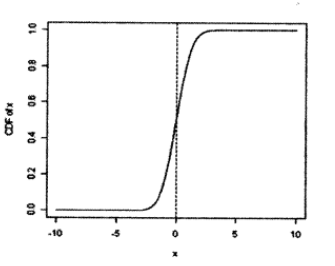
\includegraphics[width=0.2\textwidth]{images/CDF-1.png}
        \item 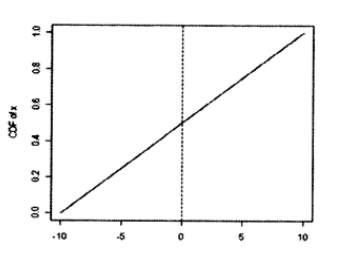
\includegraphics[width=0.2\textwidth]{images/CDF-2.png}
        \item 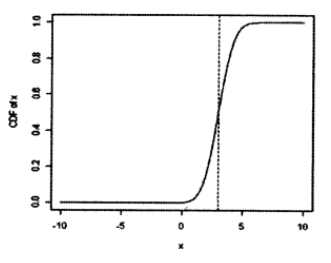
\includegraphics[width=0.2\textwidth]{images/CDF-3.png}
        \item 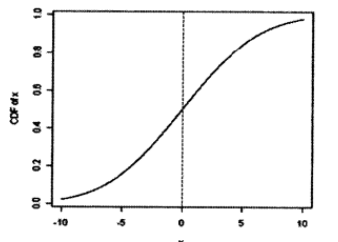
\includegraphics[width=0.2\textwidth]{images/CDF-4.png}
    \end{choices}
    
    \begin{correctanswer}
        B
    \end{correctanswer}

    \begin{explanation}
        \textbf{通过CDF形状判断方差大小的方法：}
        \begin{itemize}
            \item CDF曲线的斜率反映了概率密度函数(PDF)的高度。斜率越大，表示该点的概率密度越高。
            \item 对于具有相同取值范围[-10,10]的随机变量，方差越大意味着：
                \begin{itemize}
                    \item CDF在均值附近的斜率（上升速度）相对较小，表示数据在均值附近的集中程度较低
                    \item CDF在尾部区域的斜率相对较大，表示有更多的观测值分布在远离均值的区域
                \end{itemize}
            \item 观察四个图形：
                \begin{itemize}
                    \item 图A的CDF在均值附近上升较快，尾部较薄，表示数据集中在均值附近
                    \item 图B的CDF在均值附近上升较缓慢，且在两端都有明显的概率密度，说明数据分散程度最大
                    \item 图C和图D的CDF形状介于A和B之间，表示其方差也介于两者之间
                \end{itemize}
            \item 因此，图B代表的分布具有最大的方差，B选项正确。
        \end{itemize}
    \end{explanation}
    
    \checklist{累积分布函数（CDF）的性质与随机变量方差的关系（关键是理解CDF的形状如何反映随机变量取值的分散程度）}




\begin{question}
    The risk manager of a global macro - investment fund is currently evaluating the performance of the international portfolio managers. The annualized total returns of a selected sample of these managers are 23\%, 19\%, 13\%, 20\%, 17\%. What is the appropriate unbiased sample variance of the returns data?
    \end{question}
    
    \begin{choices}
        \item 0.00158
        \item 0.00148
        \item 0.00138
        \item 0.00128
    \end{choices}
    
    \begin{correctanswer}
        A
    \end{correctanswer}
    
    \begin{explanation}
   
    \textbf{步骤1：计算样本均值 \(\bar{x}\)}
    \begin{itemize}
    \item 样本数据为 \(x_1 = 0.23\)，\(x_2=0.19\)，\(x_3 = 0.13\)，\(x_4=0.20\)，\(x_5 = 0.17\)。
    \item 样本均值 \(\bar{x}=\frac{0.23 + 0.19+0.13+0.20+0.17}{5}=\frac{0.92}{5}=0.184\)。
    \end{itemize}
    \textbf{步骤2：计算 \((x_{i}-\bar{x})^{2}\) 并求和}
    \begin{align*}
        \sum_{i=1}^{5} (x_i - \bar{x})^2 &= (0.23 - 0.184)^2 + (0.19 - 0.184)^2 \\
                                          &\quad + (0.13 - 0.184)^2 + (0.20 - 0.184)^2 \\
                                          &\quad + (0.17 - 0.184)^2 \\
                                          &= 0.00552
        \end{align*}
    \textbf{步骤3：计算样本方差 \(s^{2}\)}
    \begin{itemize}
    \item 因为 \(n = 5\)，根据公式 \(s^{2}=\frac{\sum_{i = 1}^{n}(x_{i}-\bar{x})^{2}}{n - 1}\)，可得 \(s^{2}=\frac{0.00552}{4}=0.00138\)。
    \end{itemize}
    \end{explanation}
    
    \checklist{样本方差的计算（掌握样本方差公式）}

\begin{question}
    A financial analyst at a large asset - management firm is examining the return distributions of two portfolios over the same time frame. The analyst has collected the following data:
    \begin{center}
    \begin{tabular}{|c|c|c|}
    \hline
    Portfolio & Skewness & Kurtosis \\
    \hline
    C & - 1.2 & 1.5 \\
    \hline
    D & 0.9 & 3.5 \\
    \hline
    \end{tabular}
    \end{center}
    The analyst claims that the distribution of Portfolio C is more peaked than a normal distribution and that the distribution of Portfolio D has a long tail on the left - hand side. Which of the following statements is true?
    \end{question}
    
    \begin{choices}
        \item The analyst's claim is wrong for both portfolios.
        \item The analyst's claim is correct for Portfolio C but wrong for Portfolio D.
        \item The analyst's claim is wrong for Portfolio C but correct for Portfolio D.
        \item The analyst's claim is correct for both portfolios.
    \end{choices}
    
    \begin{correctanswer}
        A
    \end{correctanswer}
    
    \begin{explanation}
    \textbf{A选项正确。}
    \begin{itemize}
    \item 对于偏度（Skewness）和峰度（Kurtosis）的性质：
        - 正态分布的峰度为3，当峰度大于3时，分布比正态分布更尖峰（leptokurtic）；当峰度小于3时，分布比正态分布更平坦（platykurtic）。
        - 当偏度大于0时，分布有右长尾（right - skewed）；当偏度小于0时，分布有左长尾（left - skewed）。
    \item 对于投资组合C：
        - 其峰度为1.5，小于3，说明分布比正态分布更平坦，而不是更尖峰，所以分析师关于投资组合C的说法错误。
    \item 对于投资组合D：
        - 其偏度为0.9，大于0，说明分布有右长尾，而不是左长尾，所以分析师关于投资组合D的说法错误。
    \end{itemize}
    \end{explanation}
    
    \checklist{偏度和峰度的概念及应用（关键是理解偏度和峰度与分布形状的关系）}

\begin{question}
    A risk analyst at an investment bank is comparing different probability distributions to assess the likelihood of a variable exceeding a specified extreme value. Given that all the distributions have the same mean and variance, and the extreme value \(X\) is greater than the mean, which type of distribution will yield the lowest probability for the variable to exceed \(X\)?
    \end{question}
    
    \begin{choices}
        \item A platykurtic distribution
        \item A normal distribution
        \item A leptokurtic distribution with a kurtosis of 5
        \item A leptokurtic distribution with a kurtosis of 10
    \end{choices}
    
    \begin{correctanswer}
        A
    \end{correctanswer}
    
    \begin{explanation}
    \textbf{A选项正确。}
    \begin{itemize}
    \item 峰度（Kurtosis）描述了分布的尾部厚度和峰值的尖锐程度。
    \item 正态分布的峰度为3。
    \item leptokurtic分布的峰度大于3，意味着它有更厚的尾部和更尖锐的峰值。厚尾部表示极端值出现的概率更高。而且，峰度值越大，尾部越厚，极端值出现的概率也就越高。
    \item platykurtic分布的峰度小于3，其尾部比正态分布更薄，这意味着极端值出现的概率更低。
    \end{itemize}
    本题中，要找变量超过指定极端值 \(X\)（\(X\)大于均值）的概率最低的分布，由于platykurtic分布尾部最薄，所以它产生的该概率最低，故选项A正确。
    \end{explanation}
    
    \checklist{不同峰度分布的特点及极端值概率的比较（理解峰度与分布尾部厚度的关系）}

    \begin{question}
        A financial analyst at a research firm is analyzing the return distribution of a particular company over a certain period. After conducting some calculations, the analyst discovers that the median return is 4.6\%, the mean return is 4.1\%, and the mode return is 4.9\%. Additionally, the calculated measure of kurtosis is 2.2. Based on this information, which of the following correctly characterizes the distribution of returns over time?
        \end{question}
        
        \begin{choices}
            \item Negative Platykurtic
            \item Positive Leptokurtic
            \item Positive Platykurtic
            \item Negative Leptokurtic
        \end{choices}
        
        \begin{correctanswer}
            A
        \end{correctanswer}
        
        \begin{explanation}
        \textbf{A选项正确。}
        \begin{itemize}
        \item 偏度（Skewness）的判断：当均值小于中位数小于众数时，分布呈现负偏态（Negative skewness）。本题中均值\(4.1\%\)小于中位数\(4.6\%\)小于众数\(4.9\%\)，所以分布是负偏态的。
        \item 峰度（Kurtosis）的判断：当峰度小于3时，分布为低峰态（Platykurtic）。本题中峰度为\(2.2\)，小于3，所以分布是低峰态的。
        \end{itemize}
        \end{explanation}
        
        \checklist{偏度和峰度的判断（关键是掌握均值、中位数、众数与偏度的关系，以及峰度与分布形态的关系）}

\begin{question}
    A risk analyst named Lily, FRM, is working for a consulting firm. She has been tasked by a client company to assess an equity investment and creates a continuous distribution for its return performance. Lily calculates the following statistics for the distribution:
    \begin{itemize}
    \item Mean:8.2\%
    \item Median:5.5\%
    \item Excess kurtosis:2.785
    \end{itemize}
    Which of the following statements about skewness and kurtosis is most likely correct?
    \end{question}
    
    \begin{choices}
        \item Positively skewed, Leptokurtic
        \item Negatively skewed, Platykurtic
        \item Positively skewed, Platykurtic
        \item Negatively skewed, Leptokurtic
    \end{choices}
    
    \begin{correctanswer}
    A
    \end{correctanswer}
    
    \begin{explanation}
    \textbf{判断偏度（Skewness）}：
    \begin{itemize}
    \item 当均值小于中位数时，数据呈负偏态；当均值大于中位数时，数据呈正偏态。这里均值\(8.2\%\)大于中位数\(5.5\%\) ，所以数据是正偏态（Positively skewed）。
    \end{itemize}
    \textbf{判断峰度（Kurtosis）}：
    \begin{itemize}
    \item 峰度分为正态峰度（Mesokurtic）、尖峰（Leptokurtic）和平峰（Platykurtic）。超额峰度（Excess kurtosis）大于\(0\)时为尖峰，小于\(0\)时为平峰。这里超额峰度\(2.785>0\)，所以是尖峰（Leptokurtic）。
    \end{itemize}
    所以选项A正确。
    
    \checklist{偏度和峰度的判断（依据均值与中位数的关系判断偏度类型，依据超额峰度的值判断峰度类型）}
    \end{explanation}

\begin{question}
    A risk analyst at an asset management firm is evaluating the return distribution of a particular investment fund. This return distribution has the same mean and variance as a normal distribution. However, it has a significant number of data points in both tails, and there are more observations in the right - hand tail than in the left - hand tail. Which of the following statements accurately characterizes this distribution?
    \end{question}
    
    \begin{choices}
        \item Negatively skewed and Platykurtic.
        \item Positively skewed and Leptokurtic.
        \item Negatively skewed and Leptokurtic.
        \item Positively skewed and Platykurtic.
    \end{choices}
    
    \begin{correctanswer}
        B
    \end{correctanswer}
    
    \begin{explanation}
    \textbf{B选项正确。}
    \begin{itemize}
        \item 正偏态分布（Positively skewed）的特点是右尾长于左尾，即右尾的观测值更多，符合本题中右尾观测值多于左尾的情况。
        \item 尖峰态分布（Leptokurtic）的峰度大于正态分布，意味着分布在均值附近更集中，同时在尾部有更多的观测值，与本题中尾部有大量观测值的描述相符。
    \end{itemize}
    \end{explanation}
    
    \checklist{分布的偏态和峰态特征（根据分布的特征描述判断偏度和峰度类型）}
    
    \begin{question}
        A risk analyst at an equity hedge fund is assessing the characteristics of monthly stock return data. The analyst uses a sample with a size of 380. The following summarized statistics are obtained:
        \begin{center}
        \begin{tabular}{|c|c|}
        \hline
        Statistics & Monthly Return \\
        \hline
        Mean & 0.92\% \\
        \hline
        Standard Deviation & 5.42\% \\
        \hline
        $\sum_{i = 1}^{380}(R_i-\bar{R})^3$ & - 0.027 \\
        \hline
        $\sum_{i = 1}^{380}(R_i-\bar{R})^4$ & 0.0032 \\
        \hline
        $n$ & 380 \\
        \hline
        \end{tabular}
        \end{center}
        What is the sample kurtosis?
        \end{question}
        
        \begin{choices}
            \item 1.38
            \item 1.21
            \item 0.95
            \item 1.02
        \end{choices}
        
        \begin{correctanswer}
            A
        \end{correctanswer}
        
        \begin{explanation}
        \textbf{步骤1：明确样本峰度的计算公式。}
        \begin{itemize}
        \item 样本峰度（Sample kurtosis）的计算公式为：\(K=\frac{\sum_{i = 1}^{n}(R_i-\bar{R})^4}{n\times s^4}\)，其中\(R_i\)是第\(i\)个观测值，\(\bar{R}\)是样本均值，\(n\)是样本数量，\(s\)是样本标准差。
        \item 已知\(n = 380\)，\(\sum_{i = 1}^{380}(R_i-\bar{R})^4=0.0032\)，\(s = 5.42\%=0.0542\)。
        \end{itemize}
        \textbf{步骤2：代入数据计算样本峰度。}
        \begin{itemize}
        \item 将数据代入公式可得：\(K=\frac{0.0032}{380\times(0.0542)^4}\)
        \item 计算可得\(K\approx1.38\)。
        \end{itemize}
        \end{explanation}
        
        \checklist{样本峰度的计算（掌握样本峰度的计算公式）}

\begin{question}
    A risk analyst at a bank knows that the true distribution of returns is leptokurtic. When calculating the Value at Risk (VaR) assuming normality, which of the following statements is true?
    \end{question}
    
    \begin{choices}
        \item The 99\% VaR is overstated.
        \item The 99\% VaR is understated.
        \item The 99\% VaR is appropriate.
        \item We cannot state the relationship between the true VaR and the calculated VaR.
    \end{choices}
    
    \begin{correctanswer}
    B
    \end{correctanswer}
    
    \begin{explanation}
    \textbf{B选项错误。}
    \begin{itemize}
    \item leptokurtic distribution相对正态分布尾部更厚，意味着极端事件发生的概率比正态分布要高。在计算VaR时，假设正态分布会低估极端事件的概率，从而导致计算出的VaR值小于真实的VaR值，即VaR被低估了，所以选项B错误。
    \end{itemize}
    \end{explanation}
    
    \checklist{分布的尾部特征（理解厚尾分布与正态分布在极端事件概率上的差异）}


        \begin{question}
            An analyst at a quantitative investment firm is studying the relationship between two random variables. Given that a random variable \(X\) follows a normal distribution, and \(Y = C + D X\), where \(C\) and \(D\) are constants and \(D\) is negative. Which of the following statements is correct?
        \end{question}
        
        \begin{choices}
            \item The skewness of \(Y\) is identical to the skewness of \(X\).
            \item The mean of \(Y\) is identical to the mean of \(X\).
            \item The kurtosis is not affected by decreasing linear transformations.
            \item The location shift of \(C\) has an impact on the variance of \(Y\).
        \end{choices}
        
        \begin{correctanswer}
            C
        \end{correctanswer}
        
        \begin{explanation}
        \textbf{A选项错误。}
        \begin{itemize}
            \item 对于线性变换\(Y = C + D X\)，偏度（Skewness）会受到\(D\)的影响。由于\(D\)为负，\(Y\)的偏度方向会与\(X\)相反，因此偏度不再相同。
        \end{itemize}
        
        \textbf{B选项错误。}
        \begin{itemize}
            \item 设\(X\)的均值为\(\mu_X\)，则\(Y\)的均值\(\mu_Y=E(Y)=E(C + D X)=C + D\mu_X\)。
            由于\(C\)和\(D\)的存在，\(\mu_Y\)一般不等于\(\mu_X\)，所以该选项错误。
        \end{itemize}
             \textbf{C选项正确。}
        \begin{itemize}
            \item 峰度（Kurtosis）不会受到线性变换的影响。设随机变量 \(X\) 的峰度为 \(K_X\)，对于线性变换 \(Y = a + bX\)，其峰度 \(K_Y\) 计算如下：
            \begin{align*}
            K_Y &= \frac{E[(Y-\mu_Y)^4]}{[E(Y-\mu_Y)^2]^2} = \frac{E[(bX-b\mu_X)^4]}{[E(bX-b\mu_X)^2]^2} \\
                &= \frac{b^4E[(X-\mu_X)^4]}{(b^2E[(X-\mu_X)^2])^2} \\
                &= \frac{E[(X-\mu_X)^4]}{[E(X-\mu_X)^2]^2} \\
                &= K_X
            \end{align*}
            \item 从上述推导可以看出，位置参数 \(a\) 在计算中被消去，而比例参数 \(b\) 在分子和分母中相互抵消，因此线性变换不会改变峰度值。
        \end{itemize}
        
        \textbf{D选项错误。}
        \begin{itemize}
            \item 设\(X\)的方差为\(\sigma_X^2\)，则\(Y\)的方差\(\text{Var}(Y)=\text{Var}(C + D X)=D^2\text{Var}(X)\)。
            可以看出方差只与\(D\)有关，与\(C\)无关，即位置平移\(C\)不会影响\(Y\)的方差，所以该选项错误。
        \end{itemize}
        \end{explanation}
        
        \checklist{线性变换对随机变量均值、方差、偏度和峰度的影响（峰度是不受线性变化影响的）}

\begin{question}
    A risk analyst named Amy, FRM, working at a financial group, is analyzing a financial product. She denotes its return as \(X\). After gathering market data, she calculates the four named moments of \(X\) as follows:
    \begin{center}
    \begin{tabular}{|l|l|}
    \hline
    Moments & Values \\
    \hline
    Expectation & 10 \\
    \hline
    Variance & 16 \\
    \hline
    Skewness & - 5 \\
    \hline
    Kurtosis & 7 \\
    \hline
    \end{tabular}
    \end{center}
    Coincidentally, she finds another financial product \(Y\), whose return has a perfect linear relationship \(Y = - 4X+15\). Which of the following statements regarding \(Y\) is NOT correct?
    \end{question}
    
    \begin{choices}
        \item The expectation of \(Y\) equals to -25.
        \item The standard deviation of \(Y\) equals to 16.
        \item The skewness of \(Y\) equals to -5.
        \item The kurtosis of \(Y\) equals to 7.
    \end{choices}
    
    \begin{correctanswer}
    C
    \end{correctanswer}
    
    \begin{explanation}
    \textbf{A选项正确。}
    \begin{itemize}
    \item 根据期望的性质\(E(a + bX)=a + bE(X)\)，已知\(Y=-4X + 15\)，\(E(X)=10\)，则\(E(Y)=-4\times10 + 15=-25\)。
    \end{itemize}
    \textbf{B选项错误。}
    \begin{itemize}
    \item 根据方差的性质\(Var(a + bX)=b^{2}Var(X)\)，\(Var(Y)=(-4)^{2}\times16 = 256\)，那么\(Y\)的标准差\(\sigma_{Y}=\sqrt{Var(Y)}=\sqrt{256}=16\)。
    \end{itemize}
    \textbf{C选项正确。}
    \begin{itemize}
    \item 当随机变量存在线性关系\(Y = a + bX\)（\(b<0\)）时，\(Y\)的偏度与\(X\)的偏度符号相反，已知\(X\)的偏度为\(-5\)，所以\(Y\)的偏度为\(5\)。
    \end{itemize}
    \textbf{D选项正确。}
    \begin{itemize}
    \item 对于存在线性关系\(Y = a + bX\)的随机变量，峰度不变，所以\(Y\)的峰度和\(X\)的峰度相同，为\(7\)。
    \end{itemize}
    \end{explanation}
    
    \checklist{线性变换对随机变量均值、方差、偏度和峰度的影响（主要是理解偏度和峰度）}



\begin{question}
    A risk analyst at a financial institution is analyzing a set of data to understand its central tendency and dispersion. Consider the following data set:
    \begin{center}
    \begin{tabular}{|c|c|}
    \hline
    Observation & Value \\
    \hline
    1 & 0.42 \\
    \hline
    2 & 0.32 \\
    \hline
    3 & 0.31 \\
    \hline
    4 & 1.02 \\
    \hline
    5 & 0.30 \\
    \hline
    6 & 0.47 \\
    \hline
    \end{tabular}
    \end{center}
    What is the median and inter - quartile range (IQR) of this data set?
    \end{question}
    
    \begin{choices}
        \item The median is 0.37; the IQR is [0.3075, 0.4525].
        \item The median is 0.42; the IQR is [0.3175, 0.4625].
        \item The median is 0.67; the IQR is [0.3125, 0.4575].
        \item The median is 0.32; the IQR is [0.3025, 0.4475].
    \end{choices}
    
    \begin{correctanswer}
        C
    \end{correctanswer}
    
    \begin{explanation}
    \textbf{步骤1：计算中位数（Median）}
    \begin{itemize}
    \item 首先将数据从小到大排序：\(0.30, 0.31, 0.32, 0.42, 0.47, 1.02\)。
    \item 由于样本数量\(n = 6\)为偶数，中位数是中间两个数的平均值，即\(Median=\frac{0.32 + 0.42}{2}=0.37\)。
    \end{itemize}
    \textbf{步骤2：计算四分位数（Quartiles）和四分位距（IQR）}
    \begin{itemize}
    \item 下四分位数 (Q1)：数据中 25\% 的位置的值。
    \[Q1=0.31+(0.32-0.31)\times0.25=0.3125\]
    \item 上四分位数 (Q3)：数据中 75\% 的位置的值。
    \[Q3=0.42+(0.47-0.42)\times0.75=0.4525\]
    \end{itemize}
    \end{explanation}
    
    \checklist{中位数和四分位距的计算（四分位数的计算方法）}

\begin{question}
    A junior risk analyst named Leo, who is preparing for the FRM exam, is studying common measures used to describe observed data, including four named moments, quantiles, and the interquartile range. Regarding the properties of these measures, Leo makes the following statements. Which statement is correct?
    \end{question}
    
    \begin{choices}
        \item The interquartile range (IQR) is defined as the sum of the 75\% and 25\% quantiles.
        \item If random variables have heavily fat tails, the interquartile range will not be robust to apply and well-defined.
        \item The interquartile range (IQR) is typically used to measure the central tendency of the observed data.
        \item The interquartile range (IQR) is a measure of dispersion that is distinct from the standard deviation in its sensitivity to extreme values.
    \end{choices}
    
    \begin{correctanswer}
    D
    \end{correctanswer}
    
    \begin{explanation}
    \textbf{选项A错误。}
    \begin{itemize}
    \item 四分位距（interquartile range，IQR）的定义是第75百分位数（Q3）与第25百分位数（Q2）的差值，即\(IQR = Q3 - Q1\)，而不是两者之和。
    \end{itemize}
    \textbf{选项B错误。}
    \begin{itemize}
    \item 即使变量分布为严重肥尾，分位数也不受极端值影响，也可以被明确定义，具有鲁棒性。
    \end{itemize}
    \textbf{选项C错误。}
    \begin{itemize}
    \item 四分位距主要用于衡量数据的离散程度（dispersion），而不是集中趋势（central tendency），集中趋势常用均值、中位数等衡量。
    \end{itemize}
    \textbf{选项D正确。}
    \begin{itemize}
    \item 四分位距和标准差都是衡量离散程度的指标，但标准差对极端值敏感，而四分位距不受极端值影响，两者在对极端值的敏感度上是不同的。
    \end{itemize}
    \end{explanation}
    
    \checklist{四分位距IQR的定义、性质（四分位距主要用于衡量数据的离散程度）}


\begin{question}
    A risk analyst at a global investment bank is analyzing the daily returns of various financial instruments. She needs to choose appropriate descriptive statistics to summarize the return distributions, particularly when dealing with extreme market conditions. Based on the definition and properties of descriptive statistics, which of the following statements is correct?
\end{question}

\begin{choices}
    \item The arithmetic mean provides enhanced stability in return analysis by giving equal weight to all observations, making it particularly reliable during market stress periods.
    \item The median, as a positional measure, tends to better reflect the general level of returns when extreme values exist in the dataset.
    \item The mode can effectively represent the central tendency of the data, and a dataset always has a unique mode.
    \item The arithmetic mean's sensitivity to outliers makes it an optimal measure for risk assessment, as it captures the full impact of market volatility.
\end{choices}

\begin{correctanswer}
    B
\end{correctanswer}

\begin{explanation}
\textbf{A选项错误。}
\begin{itemize}
    \item 算术平均数给予所有观测值相同权重的特性实际上是其缺点而非优势。在市场压力期间，极端值会显著影响算术平均数，使其无法稳定反映收益率的一般水平。这种等权重特性反而降低了其在市场压力期间的可靠性。
\end{itemize}

\textbf{B选项正确。}
\begin{itemize}
    \item 中位数作为位置度量，不受极端值的显著影响，在金融市场动荡时期，中位数通常能更好地反映资产收益率的一般水平，例如，即使市场出现几次极端波动，中位数仍能保持稳定。
\end{itemize}

\textbf{C选项错误。}
\begin{itemize}
    \item 众数虽然可以反映数据的集中趋势，但数据集的众数并不总是唯一的，一个数据集可能有多个众数（多峰分布），也可能没有众数（均匀分布）。例如，某股票的日收益率可能在1\%和-1\%处都出现较多次数，形成双峰分布。
\end{itemize}

\textbf{D选项错误。}
\begin{itemize}
    \item 算术平均数对异常值的敏感性实际上是其局限性而非优势。在风险评估中，这种敏感性可能导致风险的错误估计，因为单个极端值就可能严重扭曲整体评估结果，使风险管理决策建立在不稳定的基础之上。
\end{itemize}
\end{explanation}

\checklist{描述性统计量的特性及其在金融数据分析中的应用（中位数在存在极端值时的优势）}


\begin{question}
    A derivatives trader at a global investment bank is pricing options on a volatile stock. She knows that Jensen's inequality is crucial for understanding why option prices differ from their intrinsic values, particularly for convex payoff functions. Based on the definition and properties of Jensen's inequality, which of the following statements is NOT correct?
\end{question}

\begin{choices}
    \item If \(h(X)\) is a convex function, then \(E[h(X)] > h(E[X])\).
    \item If \(g(X)\) is a concave function, then \(E[g(X)] < g(E[X])\).
    \item In financial derivative pricing, the expected value of a convex function is always greater than the function of the expected value.
    \item Jensen's inequality does not apply to discrete random variables.
\end{choices}

\begin{correctanswer}
    D
\end{correctanswer}

\begin{explanation}
\textbf{A选项正确。}
\begin{itemize}
    \item 这是凸函数的Jensen不等式的标准表述：如果\(h(X)\)是凸函数，则\(E[h(X)] > h(E[X])\)
    \item 在期权定价中，看涨期权的收益函数\(h(S_T)=\max(S_T-K,0)\)是凸函数，因此：
    \[E[\max(S_T-K,0)] > \max(E[S_T]-K,0)\]
    \item 这解释了为什么看涨期权的价值总是大于其内在价值
\end{itemize}

\textbf{B选项正确。}
\begin{itemize}
    \item 这是凹函数的Jensen不等式的标准表述：如果\(g(X)\)是凹函数，则\(E[g(X)] < g(E[X])\)
    \item 对于看跌期权，其收益函数\(g(S_T)=\max(K-S_T,0)\)是凸函数，通过变换\(-g(S_T)\)得到凹函数，可得：
    \[E[\max(K-S_T,0)] > \max(K-E[S_T],0)\]
    \item 这说明看跌期权的时间价值总是非负的
\end{itemize}

\textbf{C选项正确。}
\begin{itemize}
    \item 在金融衍生品定价中，对于任意凸函数\(h(X)\)，都有：
    \[E[h(X)] - h(E[X]) > 0\]
    \item 这个差值就是期权的时间价值，解释了为什么期权的市场价值通常高于其内在价值
\end{itemize}

\textbf{D选项错误。}
\begin{itemize}
    \item Jensen不等式适用于所有类型的随机变量。对于任意离散型随机变量\(X\)，其概率质量函数为\(p(x_i)\)：
    \[E[h(X)] = \sum_i h(x_i)p(x_i) > h(\sum_i x_ip(x_i)) = h(E[X])\]
    \item 对于连续型随机变量\(X\)，其概率密度函数为\(f(x)\)：
    \[E[h(X)] = \int h(x)f(x)dx > h(\int xf(x)dx) = h(E[X])\]
    \item 这个性质在金融中广泛应用，无论资产价格是连续变化还是离散跳跃
\end{itemize}
\end{explanation}

\checklist{Jensen不等式的性质及其在金融领域的应用（连续和离散都可以）}


\begin{question}
A portfolio manager at a hedge fund is analyzing the joint behavior of two asset returns during market stress periods. The manager wants to understand how extreme movements in one asset affect the other asset's returns, and is examining higher-order co-moments to improve portfolio risk management. Which of the following statements about coskewness and cokurtosis measures is correct?
\end{question}
\begin{choices}
    \item When one variable takes a clear direction whenever the other variable is large in magnitude, the coskewness between the variables will be strictly positive.
    \item Unlike skewness, the coskewness of two variables is unit-free but is not scale-free.
    \item A standardized version of the cross-fourth central moment, the calculation of cokurtosis requires raising the standard deviation of one variable to the fourth power.
    \item Cokurtosis measures the sensitivity of the magnitude of one variable to the magnitude of the other variable.
\end{choices}

\begin{correctanswer}
D
\end{correctanswer}

\begin{explanation}
\textbf{A选项错误。}
\begin{itemize}
    \item 共偏度（coskewness）不一定是严格正的。当一个变量在另一个变量取较大值时呈现明显方向性，共偏度可能为正也可能为负，这取决于两个变量之间的具体关系模式。
\end{itemize}

\textbf{B选项错误。}
\begin{itemize}
    \item 共偏度（coskewness）既是无单位的（unit-free）也是尺度不变的（scale-free）。这是因为共偏度是通过标准化的方式计算的，消除了原始变量的单位和尺度影响。
\end{itemize}

\textbf{C选项错误。}
\begin{itemize}
    \item 共峰度（cokurtosis）的计算涉及两个变量的标准差，而不是仅仅一个变量的标准差的四次方。这是一个标准化的四阶交叉矩，需要考虑两个变量的联合分布特征。
\end{itemize}

\textbf{D选项正确。}
\begin{itemize}
    \item 共峰度（cokurtosis）确实衡量了一个变量的幅度对另一个变量幅度的敏感性。它描述了两个变量极端值同时发生的倾向，这对于风险管理特别重要，因为它能帮助识别市场压力条件下的联合极端行为。
\end{itemize}
\end{explanation}

\checklist{共偏度和共峰度的特性（共偏度不一定是严格正的）}




\section{考点2：Common Univariate Random Variables 常见单变量随机变量}
\setcounter{question}{0}
\begin{question}
    A risk analyst at a fixed - income investment firm is assessing the default risk of a portfolio. The portfolio consists of seven bonds, and each bond has a 1 - year default probability of 13\%. The default events of these bonds are independent. What is the probability of exactly three bonds defaulting over the next year?
    \end{question}
    
    \begin{choices}
        \item 13.6\%
        \item 8.7\%
        \item 21.3\%
        \item 5.9\%
    \end{choices}
    
    \begin{correctanswer}
        A
    \end{correctanswer}
    
    \begin{explanation}
    \textbf{步骤1：明确二项分布公式}
    \begin{itemize}
    \item 对于独立重复试验，若每次试验成功的概率为\(p\)，失败的概率为\(q = 1 - p\)，进行\(n\)次试验，恰好有\(k\)次成功的概率公式为\(P(X = k)=C_{n}^k\times p^{k}\times q^{n - k}\)，其中\(C_{n}^k=\frac{n!}{k!(n - k)!}\)。
    \item 在本题中，\(n = 7\)（债券的数量），\(p = 0.13\)（单个债券的违约概率），\(q=1 - 0.13 = 0.87\)，\(k = 3\)（违约债券的数量）。
    \end{itemize}
    \textbf{步骤2：计算概率 \(P(X = 3)\) }
        \[
        P(X = 3) = C_{7}^3 \times (0.13)^{3} \times (0.87)^{4} = \frac{7!}{3!(7 - 3)!} \times (0.13)^{3} \times (0.87)^{4} = 13.6\%
        \]
    \end{explanation}
    
    \checklist{二项分布概率的计算（二项分布概率公式）}

\begin{question}
    A financial advisor is evaluating a binomial - distributed investment scenario. In this scenario, the probability of each success, \(p = 0.07\), and the total number of trials, \(n = 25\) trials. What is the inverse cumulative distribution function associated with a probability of 30.0\%?
    \end{question}
    
    \begin{choices}
        \item Two successes
        \item Zero successes
        \item One success
        \item Three successes
    \end{choices}
    
    \begin{correctanswer}
        C
    \end{correctanswer}
    
    \begin{explanation}
    \textbf{步骤1：明确二项分布累积分布函数公式}
    \begin{itemize}
    \item 二项分布的累积分布函数\(F(k;n,p)=\sum_{i = 0}^{k}C_{n}^i\times p^{i}\times(1 - p)^{n - i}\)，其中\(C_{n}^i=\frac{n!}{i!(n - i)!}\)，\(n\)是试验次数，\(p\)是每次试验成功的概率，\(k\)是成功的次数。
    \end{itemize}
    \textbf{步骤2：分别计算不同\(k\)值下的累积分布函数值}
    \begin{itemize}
        \item 当\(k = 0\)时：
        \begin{align*}
        F(0; 25, 0.07) &= C_{25}^0 \times (0.07)^{0} \times (0.93)^{25} \\
                        &= \frac{25!}{0!(25 - 0)!} \times (0.07)^{0} \times (0.93)^{25} \\
                        &= 1 \times 1 \times (0.93)^{25} \\
                        &\approx 0.163
        \end{align*}
        
        \item 当\(k = 1\)时：
        \begin{align*}
        F(1; 25, 0.07) &= F(0; 25, 0.07) + C_{25}^1 \times (0.07)^{1} \times (0.93)^{24} \\
                        &\approx 0.163 + 0.306 \\
                        &= 0.306
        \end{align*}
    \item 当\(k = 2\)时：
        \(F(2; 25, 0.07) > F(1; 25, 0.07) \)
    \item 当\(k = 3\)时：
        \(F(3; 25, 0.07) > F(2; 25, 0.07) > F(1; 25, 0.07)\)
    \end{itemize}
    \textbf{步骤3：确定逆累积分布函数值}
    \begin{itemize}
    \item 逆累积分布函数是找到使得累积分布函数值首次大于或等于给定概率的最小\(k\)值。
    \item 给定概率为\(30\%\)，由于\(F(0;25,0.07)<0.3\)，而\(F(1;25,0.07)>0.3\)，所以逆累积分布函数对应的成功次数为\(1\)。
    \end{itemize}
    \end{explanation}
    
    \checklist{二项分布逆累积分布函数的计算（二项分布累积分布函数公式和逆累积分布函数定义）}

\begin{question}
    A risk analyst at a large investment bank is assessing a portfolio of corporate bonds. All the bonds in the portfolio have an identical annualized probability of default, and the default events of these bonds are independent. Which type of distribution does the number of defaults in this portfolio over the next year follow?
    \end{question}
    
    \begin{choices}
        \item Exponential
        \item Binomial
        \item Normal
        \item Bernoulli
    \end{choices}
    
    \begin{correctanswer}
        B
    \end{correctanswer}
    
    \begin{explanation}
    \textbf{A选项错误。}
    \begin{itemize}
    \item 指数分布（Exponential distribution）通常用于描述事件发生的时间间隔，例如两次违约事件之间的时间间隔，而不是在给定时间内违约事件发生的次数，所以该选项不符合本题情境。
    \end{itemize}
    \textbf{B选项正确。}
    \begin{itemize}
    \item 二项分布（Binomial distribution）适用于\(n\)次独立的伯努利试验，每次试验有两种可能的结果（成功或失败），且每次试验成功的概率\(p\)相同。
    \item 在本题中，每一个债券的违约情况可以看作一次伯努利试验（违约为成功，不违约为失败），债券的总数\(n\)是固定的，每个债券的违约概率\(p\)相同且违约事件相互独立，所以一年内违约债券的数量符合二项分布。
    \end{itemize}
    \textbf{C选项错误。}
    \begin{itemize}
    \item 正态分布（Normal distribution）通常用于描述大量独立随机变量的和，当\(n\)很大且\(np\)和\(n(1 - p)\)都足够大时，二项分布可以近似为正态分布，但本题并没有提及\(n\)足够大等条件，所以不能直接说违约数量服从正态分布。
    \end{itemize}
    \textbf{D选项错误。}
    \begin{itemize}
    \item 伯努利分布（Bernoulli distribution）描述的是单次试验的结果，只有两种可能（成功或失败），而本题是要描述多个债券（多次试验）中违约的数量，不是单次试验的结果，所以不服从伯努利分布。
    \end{itemize}
    \end{explanation}
    
    \checklist{不同概率分布的适用场景（二项分布的定义及应用）}

    \begin{question}
        A junior analyst at a financial research firm is studying probability distributions and their convergence properties. Which of the following distributions does NOT tend to approximate the normal distribution as one of its parameters increases?
        \end{question}
        
        \begin{choices}
            \item Bernoulli
            \item Poisson
            \item Binomial
            \item All of the above
        \end{choices}
        
        \begin{correctanswer}
        A
        \end{correctanswer}
        
        \begin{explanation}
        \textbf{A选项正确。}
        \begin{itemize}
        \item 伯努利分布（Bernoulli distribution）是一种离散概率分布，只有两个可能的结果（成功或失败），其参数为成功的概率 \(p\)。无论参数 \(p\) 如何变化，伯努利分布本身都不会趋近于正态分布，它始终是一个两点分布，所以选项A符合题意。
        \end{itemize}
        \textbf{B选项错误。}
        \begin{itemize}
        \item 泊松分布（Poisson distribution）的参数为 \(\lambda\)，当 \(\lambda\) 增大时（一般认为 \(\lambda\geq 10\)），泊松分布可以用正态分布来近似，所以选项B不符合题意。
        \end{itemize}
        \textbf{C选项错误。}
        \begin{itemize}
        \item 二项分布（Binomial distribution）的参数为 \(n\)（试验次数）和 \(p\)（每次试验成功的概率），当 \(n\) 足够大且 \(np\geq 5\) 以及 \(n(1 - p)\geq 5\) 时，二项分布 \(X\sim B(n,p)\) 可以近似为正态分布 \(N(np,np(1 - p))\)，所以选项C不符合题意。
        \end{itemize}
        \textbf{D选项错误。}
        \begin{itemize}
        \item 只有伯努利分布不会趋近于正态分布，所以选项D错误。
        \end{itemize}
        \end{explanation}
        
        \checklist{常见概率分布与正态分布的关系（分布极限是正态）}


\begin{question}
    An investor is taking a multiple - choice quiz on financial knowledge. The quiz has eight questions, and each question has four choices. If the investor needs at least two correct answers to pass the quiz, what is the probability that the investor will pass simply by guessing?
    \end{question}
    
    \begin{choices}
        \item 20.1\%
        \item 67.8\%
        \item 0.8\%
        \item 79.6\%
    \end{choices}
    
    \begin{correctanswer}
        D
    \end{correctanswer}
    
    \begin{explanation}
    \textbf{步骤1：确定二项分布参数}
    \begin{itemize}
    \item 本题可看作二项分布问题，设答对题目为成功事件。试验次数\(n = 8\)（题目数量），每次试验成功的概率\(p=\frac{1}{4}=0.25\)（每题猜对的概率）。
    \item 二项分布概率公式为\(P(X = k)=C_{n}^k\times p^{k}\times(1 - p)^{n - k}\)，其中\(C_{n}^k=\frac{n!}{k!(n - k)!}\)。
    \end{itemize}
    \textbf{步骤2：计算通过考试的概率}
    \begin{itemize}
    \item 因为至少答对\(2\)题才能通过考试，所以\(P(X\geq2)=1 - P(X = 0)-P(X = 1)\)。
    \item 当\(k = 0\)时：
        - \(C_{8}^0=\frac{8!}{0!(8 - 0)!}=1\)，\(P(X = 0)=C_{8}^0\times(0.25)^{0}\times(0.75)^{8}\approx0.100\)。
    \item 当\(k = 1\)时：
        - \(C_{8}^1=\frac{8!}{1!(8 - 1)!}=8\)，\(P(X = 1)=C_{8}^1\times(0.25)^{1}\times(0.75)^{7}\approx0.104\)。
    \item 则\(P(X\geq2)=1-(0.100 + 0.104)=0.796 = 79.6\%\)。
    \end{itemize}
    \end{explanation}
    
    \checklist{二项分布概率的计算（确定二项分布参数并利用对立事件简化计算）}

\begin{question}
    A risk analyst at a financial institution is conducting central tendency and dispersion analysis. The probability of a single - day exceedance (default) is 1.2\%. The analyst measures the mean and standard deviation of the distribution of exceedances over a period of 350 trading days. What are the mean and standard deviation of the number of exceedances?
    \end{question}
    
    \begin{choices}
        \item Mean = 4.2, standard deviation = 2.04
        \item Mean = 3.5, standard deviation = 1.87
        \item Mean = 4.2, standard deviation = 1.87
        \item Mean = 3.5, standard deviation = 2.04
    \end{choices}
    
    \begin{correctanswer}
    A
    \end{correctanswer}
    
    \begin{explanation}
    \textbf{步骤1：明确分布类型及相关公式}
    \begin{itemize}
    \item 超过次数（违约次数）服从二项分布。
    \end{itemize}
    \textbf{步骤2：计算新的均值和标准差}
    \begin{itemize}
    \item 已知\(n = 350\)，\(p=0.012\)
    \item 均值\(\lambda=np=350\times0.012 = 4.2\)
    \item 标准差\(\sigma=\sqrt{np(1-p)}=\sqrt{350\times0.012\times(1-0.012)}=2.04\)
    \end{itemize}
    \end{explanation}
    
    \checklist{二项分布的均值和标准差计算（简单用计算公式）}    

\begin{question}
    A customer service manager at an insurance call center knows that the call center receives an average of three phone calls per hour. What is the probability that the call center will receive 24 calls in a 7 - hour period?
    \end{question}
    
    \begin{choices}
        \item 6.40\%
        \item 3.66\%
        \item 5.59\%
        \item 16.56\%
    \end{choices}
    
    \begin{correctanswer}
        C
    \end{correctanswer}
    
    \begin{explanation}
    \textbf{步骤1：确定泊松分布参数}
    \begin{itemize}
    \item 泊松分布适用于描述在固定时间或空间内事件发生的次数，其概率质量函数为\(P(X = k)=\frac{\lambda^{k}e^{-\lambda}}{k!}\)，其中\(\lambda\)是给定时间或空间内事件发生的平均次数，\(k\)是实际发生的事件次数。
    \item 已知每小时平均接到\(3\)个电话，那么\(7\)小时内平均接到的电话数\(\lambda=3\times7 = 21\)。本题中\(k = 24\)（即\(7\)小时内实际接到\(24\)个电话）。
    \end{itemize}
    \textbf{步骤2：计算概率}
    \begin{itemize}
    \item 将\(\lambda = 21\)，\(k = 24\)代入泊松分布公式\(P(X = 24)=\frac{21^{24}e^{-21}}{24!}\)。
    \item 计算可得\(P(X = 24)\approx0.0559 = 5.59\%\)。
    \end{itemize}
    \end{explanation}
    
    \checklist{泊松分布概率的计算（确定泊松分布的参数\(\lambda\)并正确代入公式计算）}
    
    \begin{question}
        A risk analyst at a financial institution is assessing the operational risk of a low - severity administrative process. This process typically generates an average of 12 errors per week (with each week consisting of five workdays). If the loss frequency of this process follows a Poisson distribution, which value is NEAREST to the probability that more than one error will occur tomorrow; i.e., \(P(K > 1|\lambda=\frac{12}{5})\)?
        \end{question}
        
        \begin{choices}
            \item 47.51\%
            \item 66.16\%
            \item 20.19\%
            \item 32.30\%
        \end{choices}
        
        \begin{correctanswer}
            B
        \end{correctanswer}
        
        \begin{explanation}
        \textbf{步骤1：确定泊松分布参数}
        \begin{itemize}
        \item 已知每周平均产生\(12\)个错误，每周工作\(5\)天，则每天平均产生的错误数\(\lambda=\frac{12}{5} = 2.4\)。
        \end{itemize}
        \textbf{步骤2：根据泊松分布概率公式计算}
        \begin{itemize}
        \item 泊松分布的概率公式为\(P(K = k)=\frac{e^{-\lambda}\lambda^{k}}{k!}\)，其中\(K\)表示事件发生的次数，\(\lambda\)是平均发生次数，\(k\)是具体的发生次数。
        \item 要求\(P(K>1)\)，根据概率的性质\(P(K > 1)=1 - P(K\leq1)=1-(P(K = 0)+P(K = 1))\)。
        \item 当\(k = 0\)时，\(P(K = 0)=\frac{e^{-2.4}\times2.4^{0}}{0!}=0.0907\)。
        \item 当\(k = 1\)时，\(P(K = 1)=\frac{e^{-2.4}\times2.4^{1}}{1!}=0.2177\)。
        \item 则\(P(K\leq 1)=P(K = 0)+P(K = 1)=0.0907 + 0.2177=0.3084\)。
        \item 所以\(P(K > 1)=1 - 0.3084 = 0.6916\)，B选项正确。
        \end{itemize}
        \end{explanation}
        
        \checklist{泊松分布的概率计算（利用概率性质转化问题）}

\begin{question}
    An operational risk manager at a bank is using the Poisson distribution to estimate the frequency of losses exceeding USD 3 million in the next two - year period. Based on historical data from the past 12 years, the average frequency of losses greater than USD 3 million is 2 per year. Assuming that the past data is a good indicator of future events and all losses are independent, what is the probability of at most one loss over USD 3 million occurring during the next two years?
    \end{question}
    
    \begin{choices}
        \item 8.74\%
        \item 8.61\%
        \item 9.40\%
        \item 9.16\%
    \end{choices}
    
    \begin{correctanswer}
        D
    \end{correctanswer}
    
    \begin{explanation}
    \textbf{步骤1：确定泊松分布的参数\(\lambda\)。}
    \begin{itemize}
        \item 泊松分布的参数\(\lambda\)表示在给定时间间隔内事件发生的平均次数。已知平均每年损失超过300万美元的次数为2次，要求的是未来两年的情况，所以\(\lambda = 2\times2=4\)。
    \end{itemize}
    \textbf{步骤2：计算泊松分布的概率公式。}
    \begin{itemize}
        \item 泊松分布的概率质量函数为\(P(X = k)=\frac{e^{-\lambda}\lambda^{k}}{k!}\)，其中\(X\)表示事件发生的次数，\(k\)为具体的次数。
        \item \(P(X\leq1)=P(X = 0)+P(X = 1)\)。
        \item 当\(k = 0\)时，\(P(X = 0)=\frac{e^{-4}\times4^{0}}{0!}=e^{-4}\)。
        \item 当\(k = 1\)时，\(P(X = 1)=\frac{e^{-4}\times4^{1}}{1!}=4e^{-4}\)。
        \item 则\(P(X\leq1)=e^{-4}+4e^{-4}=5e^{-4}\approx 9.16\%\)。
    \end{itemize}
    \end{explanation}
    
    \checklist{泊松分布的概率计算（先确定泊松分布的参数\(\lambda\)）}

\begin{question}
    A risk manager at a financial institution is back - testing the firm's model for estimating VaR. In the previous 180 trading days, the manager observes six exceedances. Assuming that the model is correctly calibrated and all exceedances are independent of each other, what is the probability that there are exactly eight exceedances over a period of 300 trading days?
    \end{question}
    
    \begin{choices}
        \item 39.25\%
        \item 26.97\%
        \item 11.26\%
        \item 9.84\%
    \end{choices}
    
    \begin{correctanswer}
        C
    \end{correctanswer}
    
    \begin{explanation}
    \textbf{步骤1：计算单位时间的平均违约率。}
    \begin{itemize}
        \item 已知在180个交易日中出现了6次违约（exceedances），则单位时间（每天）的平均违约率\(p=\frac{6}{180}\)。
        \item 对于300个交易日，期望的违约次数\(\lambda = p\times300=\frac{6}{180}\times300=10\)。
    \end{itemize}
    \textbf{步骤2：使用泊松分布计算概率。}
    \begin{itemize}
        \item 泊松分布的概率质量函数为\(P(X = k)=\frac{e^{-\lambda}\lambda^{k}}{k!}\)，其中\(X\)表示事件发生的次数，\(k\)为具体的次数。
        \item 这里\(k = 8\)，\(\lambda=10\)，则\(P(X = 8)=\frac{e^{-10}\times10^{8}}{8!}= 11.26\%\)。
    \end{itemize}
    \end{explanation}
    
    \checklist{泊松分布概率计算（关键是根据情境确定泊松分布的参数\(\lambda\)）}



\begin{question}
    A risk analyst is dealing with random variables. Given that \(X\) is a random variable following a Poisson distribution with \(\lambda = 3\). Define a new random variable \(Y = 2 + 3X\). What are the expectation and variance for \(Y\)?
    \end{question}
    
    \begin{choices}
        \item \(E(Y)=0\), \(Var(Y)=9\)
        \item \(E(Y)=0\), \(Var(Y)= 27\)
        \item \(E(Y)=11\), \(Var(Y)=9\)
        \item \(E(Y)=11\), \(Var(Y)=27\)
    \end{choices}
    
    \begin{correctanswer}
    D
    \end{correctanswer}
    
    \begin{explanation}
    \textbf{步骤1：求\(E(X)\)和\(Var(X)\)}
    \begin{itemize}
    \item 对于泊松分布，\(E(X)=Var(X)=\lambda\)。已知\(\lambda = 3\)，所以\(E(X)=Var(X)=3\)。
    \end{itemize}
    \textbf{步骤2：求\(E(Y)\)}
    \begin{itemize}
    \item \(E(Y)=E(2 + 3X)=2+3E(X)=2 + 3\times3=11\)。
    \end{itemize}
    \textbf{步骤3：求\(Var(Y)\)}
    \begin{itemize}
    \item \(Var(Y)=Var(2 + 3X)=3^2\times3 = 27\)。
    \end{itemize}
    \end{explanation}
    
    \checklist{随机变量线性变换后的期望和方差计算（用公式去理解）}

\begin{question}
    A risk analyst at a manufacturing firm is using the firm's proprietary forecasting model. The model assumes that the random variables follow the Poisson distribution. The analyst is evaluating the probability of the number of defects in an assembly production process of another company. Given that there is a 0.008 probability of a defect for every production run, what is the probability of having 5 defects in 800 production runs?
    \end{question}
    
    \begin{choices}
        \item 12.3\%
        \item 14.9\%
        \item 16.8\%
        \item 20.5\%
    \end{choices}
    
    \begin{correctanswer}
    B
    \end{correctanswer}
    
    \begin{explanation}
    \textbf{步骤1：确定泊松分布的参数\(\lambda\)}
    \begin{itemize}
    \item 对于泊松分布\(X\sim Poisson(\lambda)\)，\(\lambda\) 表示单位时间（或单位面积等）内随机事件的平均发生次数。这里平均每次生产运行出现缺陷的概率为\(p = 0.008\)，生产运行次数\(n = 800\)，则\(\lambda=np=800\times0.008 = 6.4\)。
    \end{itemize}
    \textbf{步骤2：运用泊松分布概率公式计算概率}
    \begin{itemize}
    \item 泊松分布的概率质量函数为\(P(X = k)=\frac{e^{-\lambda}\lambda^{k}}{k!}\)，其中\(k\)是事件发生的次数，这里\(k = 5\)，\(\lambda = 6.4\)。
    \item 计算\(P(X = 5)=\frac{e^{-6.4}\times6.4^{5}}{5!} = 14.9\%\)。
    \end{itemize}
    \end{explanation}
    
    \checklist{泊松分布的概率计算（关键是确定泊松分布的参数\(\lambda\)）}




    \begin{question}
        A risk analyst at a fixed - income investment firm is evaluating five different random variables for risk assessment. The five random variables are as follows:
        \begin{itemize}
        \item A standard normal random variable; no parameters needed.
        \item A student's t - distribution with 12 degrees of freedom; df = 12.
        \item A Bernoulli variable that represents the probability of a loan default, where the probability of default (PD) = 6\%; p = 0.06.
        \item A Poisson distribution that models the frequency of system glitches in a trading day, where \(\lambda=7.0\).
        \item A binomial variable that describes the number of defaults in a portfolio of 60 bonds, each with a PD = 3\%; n = 60, p = 0.03.
        \end{itemize}
        Which of the above has, respectively, the lowest value and highest value as its variance among the set?
        \end{question}
        
        \begin{choices}
            \item Binomial (lowest) and Student's t (highest)
            \item Standard normal (lowest) and Bernoulli (highest)
            \item Poisson (lowest) and Binomial (highest)
            \item Bernoulli (lowest) and Poisson (highest)
        \end{choices}
        
        \begin{correctanswer}
            D
        \end{correctanswer}
        
        \begin{explanation}
        \textbf{步骤1：分别计算各随机变量的方差}
        \begin{itemize}
        \item 对于标准正态分布，其方差\(\sigma^{2}=1\)。
        \item 对于自由度为\(df = 12\)的学生\(t\)分布，当\(df>2\)时，其方差\(\sigma^{2}=\frac{df}{df - 2}=\frac{12}{12 - 2}=1.2\)。
        \item 对于伯努利分布，已知\(p = 0.06\)，根据方差公式\(\sigma^{2}=p(1 - p)=0.06\times(1 - 0.06)=0.06\times0.94 = 0.0564\)。
        \item 对于泊松分布，已知\(\lambda = 7\)，其方差\(\sigma^{2}=\lambda = 7\)。
        \item 对于二项分布，\(n = 60\)，\(p = 0.03\)，根据方差公式\(\sigma^{2}=np(1 - p)=60\times0.03\times(1 - 0.03)=60\times0.03\times0.97 = 1.746\)。
        \end{itemize}
        \textbf{步骤2：比较方差大小并确定最低和最高方差的分布}
        \begin{itemize}
        \item 通过比较\(0.0564<1<1.2<1.746<7\)，可知伯努利分布方差最低，泊松分布方差最高。
        \end{itemize}
        \end{explanation}
        
        \checklist{不同概率分布方差的计算与比较（标准正态分布、学生\(t\)分布、伯努利分布、泊松分布、二项分布方差计算公式）}

\begin{question}
    A risk analyst at an asset management firm is comparing a normal distribution and a Student's t - distribution that have the same mean and standard deviation. Which of the following statements about their relationship is the most accurate?
    \end{question}
    
    \begin{choices}
        \item The normal distribution and the Student's t - distribution have different skewness but the same kurtosis.
        \item The normal distribution has larger skewness and larger kurtosis compared to the Student's t - distribution.
        \item As the degrees of freedom increase, the kurtosis of the Student's t - distribution approaches that of the normal distribution.
        \item The Student's t - distribution is a good approximation for the normal distribution when the number of degrees of freedom is small.
    \end{choices}
    
    \begin{correctanswer}
        C
    \end{correctanswer}
    
    \begin{explanation}
    \textbf{A选项错误。}
    \begin{itemize}
        \item 正态分布的偏度（skewness）为0，峰度（kurtosis）为3。而学生t分布的偏度也为0，但峰度大于3（当自由度较小时），所以它们的峰度不同。
    \end{itemize}
    \textbf{B选项错误。}
    \begin{itemize}
        \item 正态分布的偏度为0，峰度为3，是一个标准的对称分布。学生t分布在自由度较小时，峰度大于3，即具有更厚的尾部。所以是学生t分布的峰度更大，而不是正态分布。
    \end{itemize}
    \textbf{C选项正确。}
    \begin{itemize}
        \item 随着自由度的增加，学生t分布的形状逐渐接近正态分布。具体来说，其峰度会逐渐收敛到正态分布的峰度值3。当自由度趋近于无穷大时，学生t分布就等同于正态分布。
    \end{itemize}
    \textbf{D选项错误。}
    \begin{itemize}
        \item 当自由度较小时，学生t分布的尾部比正态分布更厚，与正态分布差异较大。只有当自由度较大时，学生t分布才近似于正态分布，而不是自由度较小时。
    \end{itemize}
    \end{explanation}
    
    \checklist{正态分布和学生t分布的特征及关系（t分布的峰度随着自由度的增加逐渐趋近于正态分布的峰度）}

\begin{question}
    An investor is analyzing a situation similar to a quiz. Suppose there is a test with 25 true - false questions. A candidate has no knowledge of the content and randomly guesses the answers. How would you find the probability that the candidate will get 10 or fewer answers correct?
        \end{question}
        
        \begin{choices}
            \item Find the probability that \(X = 10\) in a binomial distribution with \(n = 25\) and \(p = 0.5\).
            \item Find the area between 0 and 10 in a uniform distribution that goes from 0 to 25.
            \item Find the cumulative probability for 10 in a binomial distribution with \(n = 25\) and \(p = 0.5\).
            \item Find the probability that \(X = 10\) for a normal distribution with mean of 12.5 and standard deviation of \(\sqrt{6.25}\).
        \end{choices}
        
        \begin{correctanswer}
            C
        \end{correctanswer}
        
        \begin{explanation}
        \textbf{A选项错误。}
        \begin{itemize}
        \item 题目要求的是答对10题及以下的概率，而求\(X = 10\)在二项分布中的概率，只是答对恰好10题的概率，并非答对10题及以下的概率，所以该选项不符合要求。
        \end{itemize}
        \textbf{B选项错误。}
        \begin{itemize}
        \item 本题中答题情况是二项分布，每个问题答对的概率是\(0.5\)，并非均匀分布。均匀分布不能正确描述这种有固定概率的二项试验情况，所以不能用均匀分布来计算该概率。
        \end{itemize}
        \textbf{C选项正确。}
        \begin{itemize}
        \item 对于二项分布 \(X \sim B(n,p)\)，本题中 \(n = 25\)（题目数量），\(p = 0.5\)（每题答对的概率），要求答对 10 题及以下的概率，即 \(P(X \leq 10)\)，这就是二项分布的累积概率，所以应该求在 \(n = 25\)，\(p = 0.5\) 的二项分布中 \(X = 10\) 的累积概率。
        \end{itemize}
        \textbf{D选项错误。}
        \begin{itemize}
        \item 虽然当\(n\)较大时，二项分布可以用正态分布近似，但本题直接要求求答对10题及以下的概率，用二项分布的累积概率求解更直接准确，而且求\(X = 10\)在正态分布中的概率也不符合求答对10题及以下概率的要求。
        \end{itemize}
        \end{explanation}
        
        \checklist{二项分布累积概率的应用（关键是对累积分布函数定义的理解）}

\begin{question}
    A risk analyst at an investment bank is evaluating a portfolio that consists of five bonds. Each bond has a 1 - year default probability of 22\%. The default events of these bonds are independent. What is the mean and variance of the number of bonds defaulting over the next year?
    \end{question}
    
    \begin{choices}
        \item Mean = 0.22, variance = 0.86
        \item Mean = 1.1, variance = 0.86
        \item Mean = 1.1, variance = 0.98
        \item Mean = 0.22, variance = 0.98
    \end{choices}
    
    \begin{correctanswer}
        B
    \end{correctanswer}
    
    \begin{explanation}
    \textbf{步骤1：明确分布类型}
    \begin{itemize}
    \item 由于债券违约事件相互独立，且每个债券违约概率固定，所以债券违约数量服从二项分布。设违约债券数量为\(X\)，债券总数\(n = 5\)，单个债券违约概率\(p=0.22\)，即\(X\sim B(n = 5,p = 0.22)\)。
    \end{itemize}
    \textbf{步骤2：计算均值}
    \begin{itemize}
    \item 对于二项分布\(X\sim B(n,p)\)，其均值\(\mu=np\)。
    \item 把\(n = 5\)，\(p = 0.22\)代入公式，可得\(\mu=5\times0.22 = 1.1\)。
    \end{itemize}
    \textbf{步骤3：计算方差}
    \begin{itemize}
    \item 对于二项分布\(X\sim B(n,p)\)，其方差\(\sigma^{2}=np(1 - p)\)。
    \item 将\(n = 5\)，\(p = 0.22\)代入公式，\(\sigma^{2}=5\times0.22\times(1 - 0.22)=5\times0.22\times0.78 = 0.858\approx0.86\)。
    \end{itemize}
    \end{explanation}
    
    \checklist{二项分布的均值和方差的计算（每个分布的均值和方差都应该记住）}

\begin{question}
    A risk analyst knows that the variable \(Y\) is a normal random variable with \(Y\sim N(\mu,\sigma^{2})\). Which of the following \(X\) variables is log - normally distributed?
    \end{question}
    
    \begin{choices}
        \item \(X = e^{Y}\)
        \item \(X=\mathrm{LN}(Y)\)
        \item \(X = Y(1)+Y(2)+\cdots+Y(n)\)
        \item \(X=\mathrm{LN}[Y(2)/Y(1)]\)
    \end{choices}
    
    \begin{correctanswer}
    A
    \end{correctanswer}
    
    \begin{explanation}
    \textbf{A选项正确。}
    \begin{itemize}
    \item 根据对数正态分布的定义，如果随机变量 \(Y\) 服从正态分布 \(N(\mu,\sigma^{2})\)，那么 \(X = e^{Y}\) 服从对数正态分布。因为对 \(X = e^{Y}\) 取自然对数，\(\ln(X)=Y\)，\(Y\) 是正态分布，所以 \(X\) 是对数正态分布。
    \end{itemize}
    \end{explanation}
    
    \checklist{对数正态分布的定义和性质（关键是理解对数正态分布与正态分布之间的关系）}

    \begin{question}
        Given two independent variables \( X \) and \( Y \) that follow a lognormal distribution, which of the following statements is true regarding the distribution of the product \( Z = X \times Y \)?
        \end{question}
        
        \begin{choices}
            \item The distribution of \( Z \) is Normal.
            \item The distribution of \( Z \) is Lognormal.
            \item The distribution of \( Z \) is Exponential.
            \item The distribution of \( Z \) is None of the above.
        \end{choices}
        
        \begin{correctanswer}
            B
        \end{correctanswer}
        
        \begin{explanation}
        \textbf{B选项正确。}
        \begin{itemize}
            \item \( X \) 和 \( Y \) 都是独立的对数正态分布变量，则In(X)和In(Y)服从正态分布
            \item 1n(X) +1n(Y)= 1n(XY)，1n(XY)服从正态分布，故\( X \) 和 \( Y \)的乘积 \( Z = X \times Y \) 也遵循对数正态分布。
        \end{itemize}
        \end{explanation}
        
        \checklist{正态分布和对数正态分布的性质（两个独立的正态分布变量的和仍然是正态分布）}

\begin{question}
    A financial analyst conducts a multivariate regression using a sample of 35 observations (\(n = 35\)). The regression results in five regression coefficients, including an intercept and four partial - slope coefficients. The OLS estimates follow a Student's \(t\) distribution. What are the variance and kurtosis of this Student's \(t\) distribution respectively?
    \end{question}
    
    \begin{choices}
        \item 1.00, 3.0
        \item 1.07, 3.23
        \item 1.00, 3.23
        \item 1.07, 3.0
    \end{choices}
    
    \begin{correctanswer}
    B
    \end{correctanswer}
    
    \begin{explanation}
    \textbf{步骤1：计算自由度}
    \begin{itemize}
    \item 在多元回归中，自由度\(df=n - k\)，其中\(n\)是样本数量，\(k\)是回归系数的数量（包括截距项）。这里\(n = 35\)，\(k = 5\)，所以\(df=35 - 5=30\)。
    \end{itemize}
    \textbf{步骤2：计算Student's \(t\)分布的方差}
    \begin{itemize}
    \item 对于自由度为\(df\)的Student's \(t\)分布，方差为\(\frac{df}{df - 2}\)，将\(df = 30\)代入，可得方差\(=\frac{30}{30 - 2}=\frac{30}{28}=1.07\)。
    \end{itemize}
    \textbf{步骤3：计算Student's \(t\)分布的峰度}
    \begin{itemize}
    \item 对于自由度为\(df\)的Student's \(t\)分布，峰度（kurtosis）为\(3\frac{df-2}{df - 4}\)，将\(df = 30\)代入，可得峰度\(=3\times\frac{30-2}{30 - 4}=3.23\)（考虑到计算中的近似）。
    \end{itemize}
    \end{explanation}
    
    \checklist{Student's \(t\)分布的参数计算（利用自由度计算Student's \(t\)分布的方差和峰度）}

\begin{question}
    A risk analyst is comparing the relationship between a normal distribution and a Student's t - distribution with the same mean and standard deviation. Which of the following statements is correct?
    \end{question}
    
    \begin{choices}
        \item They have the same skewness and the same kurtosis.
        \item The Student's t - distribution has a smaller skewness and a smaller kurtosis.
        \item The kurtosis of a Student's t - distribution converges to that of the normal distribution as the number of degrees of freedom increases.
        \item Given the same confidence level, t - distribution has a narrower confidence interval than the z - distribution.
    \end{choices}
    
    \begin{correctanswer}
    C
    \end{correctanswer}
    
    \begin{explanation}
    \textbf{A选项错误。}
    \begin{itemize}
    \item 正态分布和t分布的偏度都为0，但t分布的峰度比正态分布大（当自由度较小时），并非峰度相同，所以该选项错误。
    \end{itemize}
    \textbf{B选项错误。}
    \begin{itemize}
    \item 两者偏度均为0 ，并且t分布的峰度比正态分布大（自由度较小时），而不是更小，所以该选项错误。
    \end{itemize}
    \textbf{C选项正确。}
    \begin{itemize}
    \item t分布的峰度随着自由度的增加逐渐趋近于正态分布的峰度。当自由度趋于无穷大时，t分布就近似于正态分布，该选项正确。
    \end{itemize}
    \textbf{D选项错误。}
    \begin{itemize}
    \item 给定相同的置信水平，t分布的尾部比正态分布（z分布）更厚，意味着t分布的临界值更大，所以t分布的置信区间比z分布更宽，而不是更窄，该选项错误。
    \end{itemize}
    \end{explanation}
    
    \checklist{正态分布和t分布的特征比较（t分布的峰度随着自由度的增加逐渐趋近于正态分布的峰度）}


\begin{question}
    A financial analyst at an asset management firm is evaluating the use of statistical distributions for hypothesis testing in regression models. Each of the following statements regarding the chi - square and F distributions is true EXCEPT:
    \end{question}
    
    \begin{choices}
        \item Given a calculated F - ratio, where \(F=\frac{(ESS/df_1)}{(SSR/df_2)}\), along with the sample size \(n\) and the number of independent variables \(k\), one can compute the adjusted coefficient of determination \(\bar{R}^2\) in a multiple regression.
        \item The F - distribution is employed to test whether all the slope coefficients in a multiple regression are zero, determining if the overall regression model is significant.
        \item As the degrees of freedom increase, the chi - square distribution approaches a normal distribution, while the F - distribution approaches a  lognormal distribution.
        \item The chi - square distribution is utilized to test if the variance of a sample comes from a population with a pre - specified variance; that is, given an observed sample variance, is the true population variance different from a hypothesized value?
    \end{choices}
    
    \begin{correctanswer}
        C
    \end{correctanswer}
    
    \begin{explanation}
    \textbf{A选项正确。}
    \begin{itemize}
    \item 在多元回归中，调整的决定系数\(\bar{R}^2 = 1-\frac{SSR/(n - k - 1)}{SST/(n - 1)}\)，其中\(F=\frac{(ESS/df_1)}{(SSR/df_2)}\)，\(ESS\)是回归平方和，\(SSR\)是残差平方和，\(SST=ESS + SSR\)。已知\(F\)比率、样本量\(n\)和自变量个数\(k\)，可以通过\(F\)统计量与\(ESS\)、\(SSR\)的关系，进而计算出\(\bar{R}^2\)。
    \end{itemize}
    \textbf{B选项正确。}
    \begin{itemize}
    \item 在多元回归分析里，\(F\)检验用于检验原假设\(H_0:\beta_1=\beta_2=\cdots=\beta_k = 0\)，即所有斜率系数是否同时为零。若拒绝原假设，则说明回归模型整体是显著的，具有一定的解释能力。
    \end{itemize}
    \textbf{C选项错误。}
    \begin{itemize}
    \item 随着自由度的增加，卡方分布和\(F\)分布都趋近于正态分布，所以该选项表述错误。
    \end{itemize}
    \textbf{D选项正确。}
    \begin{itemize}
    \item 卡方检验常用于检验样本方差是否来自具有特定方差的总体。通过计算卡方统计量\(\chi^{2}=\frac{(n - 1)s^{2}}{\sigma^{2}}\)，其中\(n\)是样本量，\(s^{2}\)是样本方差，\(\sigma^{2}\)是假设的总体方差，然后依据卡方分布进行假设检验。
    \end{itemize}
    \end{explanation}
    
    \checklist{卡方分布和F分布的性质及在多元回归中的应用（随着自由度的增加，卡方分布和F分布都趋近于正态分布）}

\begin{question}
    A risk analyst at a fixed - income investment firm is reviewing distributions. In regard to the chi-squared and F - distribution, each of the following is true EXCEPT which is false?
    \end{question}
    
    \begin{choices}
        \item Both the chi-squared and F - distribution are non - negative and positively skewed to the right.
        \item The square of variable with a student’s t distribution with df = k has an F - distribution with 1 and k df.
        \item The sum of two independent chi-squared variables, with respectively k1 and k2 degrees of freedom, is itself chi-squared with (k1 + k2) degrees of freedom.
        \item The chi-squared distribution is approximated by the ratio of two independent F.
    \end{choices}
    
    \begin{correctanswer}
    D
    \end{correctanswer}
    
    \begin{explanation}
    \textbf{A选项正确。}
    \begin{itemize}
    \item 卡方分布和F分布的取值范围都是非负的，并且它们的概率密度函数都是右偏态的。
    \end{itemize}
    \textbf{B选项正确。}
    \begin{itemize}
    \item 如果一个变量服从自由度为k的学生t分布，那么它的平方服从自由度为1和k的F分布，这是常见的分布关系，即 $t^{2}(k)\sim F(1,k)$。
    \end{itemize}
    \textbf{C选项正确。}
    \begin{itemize}
    \item 两个独立的卡方变量，自由度分别为k1和k2 ，它们的和服从自由度为k1 + k2的卡方分布，这是卡方分布的可加性。
    \end{itemize}
    \textbf{D选项错误。}
    \begin{itemize}
    \item 卡方分布并不是由两个独立F分布的比值来近似的，F分布是两个独立的卡方随机变量的比值的分布，即$F(k_1, k_2) \sim \frac{\chi^2(1)/k_1}{\chi^2(2)/k_2}$，该选项说法错误。
    \end{itemize}
    \end{explanation}
    
    \checklist{卡方分布、F分布以及学生t分布的性质和关系（卡方分布并不是由两个独立F分布的比值来近似的）}

\begin{question}
    A junior analyst at a prestigious investment bank has been tasked with giving a presentation on commonly used distributions in finance to finance undergraduates. While preparing, the analyst identifies some frequently misunderstood concepts and plans to include a short quiz during the presentation. Which of the following statements is most likely correct?
    \end{question}
    
    \begin{choices}
        \item The graphs of PDFs (probability density functions) for lognormal distribution, $\chi^{2}$ distribution and F - distribution are alike, all of which are left - skewed and bounded from below by zero.
        \item Lognormal distribution is used to model asset returns.
        \item When two normal distributions are mixed, the mixed distribution may be skewed.
        \item T - distribution is more suitable in a joint test than F - distribution.
    \end{choices}
    
    \begin{correctanswer}
        C
    \end{correctanswer}
    
    \begin{explanation}
    \textbf{A选项错误。}
    \begin{itemize}
        \item 对数正态分布、卡方分布和F分布的概率密度函数图像是右偏态，而非左偏态，且都以零为下界。所以该选项描述错误。
    \end{itemize}
    \textbf{B选项错误。}
    \begin{itemize}
        \item 对数正态分布通常用于模拟资产价格，而不是资产收益率,资产收益率一般用正态分布等进行建模。所以该选项错误。
    \end{itemize}
    \textbf{C选项正确。}
    \begin{itemize}
        \item 当两个正态分布混合时，混合分布可能会出现偏态。因为不同参数的正态分布混合后，其整体的分布形状会受到各组成部分的影响，可能不再是对称的正态分布，从而出现偏态。所以该选项正确。
    \end{itemize}
    \textbf{D选项错误。}
    \begin{itemize}
        \item 在联合检验中，F分布更为合适，因为F分布常用于检验多个参数的联合假设。所以该选项错误。
    \end{itemize}
    \end{explanation}
    
    \checklist{各类分布的特点及应用（对数正态分布、卡方分布、F分布、t分布以及混合分布的特征）}

    \begin{question}
        An analyst at a quantitative investment firm is examining the combination of two normal distributions. Both distributions have a mean of 0, but different variances: N(0, 2) and N(0, 5). If the analyst uses the standard method to mix these two distributions, which of the following statements correctly describes the resulting mixture distribution?
        \end{question}
        
        \begin{choices}
            \item The resulting distribution will not be normal. In fact, it will be skewed and have heavy tails.
            \item The resulting distribution will also be normal, with a mean of 0 and a variance of 3.5.
            \item The resulting distribution will not be normal. In fact, it will be bimodal.
            \item The resulting distribution will not be normal. In fact, it will have extremely heavy tails.
        \end{choices}
        
        \begin{correctanswer}
            D
        \end{correctanswer}
        
        \begin{explanation}
        \textbf{步骤1：明确混合后的分布是否是正态分布}
        \begin{itemize}
        \item 两个正态分布 \(N(\mu_1,\sigma_1^{2})\) 和 \(N(\mu_2,\sigma_2^{2})\) 的混合分布，当 \(\mu_1=\mu_2\) 但 \(\sigma_1^{2}\neq\sigma_2^{2}\) 时，混合后的分布不再是正态分布，选项B错误。
        \end{itemize}
        \textbf{步骤2：分析混合分布的特征}
        \begin{itemize}
        \item 选项A错误，因为两个分布均值相同，不会产生偏态。
        \item 选项C错误，由于两个分布均值相同，混合分布不会呈现双峰形态。
        \item 选项D正确，不同方差的正态分布混合后，会使得分布在尾部的概率增大，从而具有非常重的尾部特征。
        \end{itemize}
        \end{explanation}
        
        \checklist{混合分布（不同方差的正态分布混合后有非常重的尾部特征）}



        \begin{question}
            A quantitative analyst at a hedge fund is studying the t-distribution for modeling asset returns, particularly during market stress periods when returns often exhibit fat tails. The analyst is reviewing the properties of t-distribution's probability density function (PDF) with different degrees of freedom (df). Based on the definition and properties of t-distribution, which of the following statements is NOT correct?
        \end{question}
        
        \begin{choices}
            \item The probability density function of t-distribution is parameterized by its degrees of freedom \(df\), where \(df = n-1\).
            \item The probability density function of t-distribution is bell-shaped, symmetric around zero, with tails heavier than the normal distribution.
            \item As the degrees of freedom \(df\) increases, the t-distribution's probability density function approaches the normal distribution.
            \item The probability density function of t-distribution reaches its maximum skewness when \(df = 1\).
        \end{choices}
        
        \begin{correctanswer}
            D
        \end{correctanswer}
        
        \begin{explanation}
        \textbf{A选项正确。}
        \begin{itemize}
            \item t分布的自由度\(df = n-1\)，其中n为样本量，这在金融中常用于小样本量的收益率分析，特别是在历史数据有限的情况下。
        \end{itemize}
        
        \textbf{B选项正确。}
        \begin{itemize}
            \item t分布的概率密度函数形状为钟形，且关于y轴对称，相比正态分布，t分布具有更厚的尾部，这使其更适合建模金融资产收益率的极端值。
        \end{itemize}
        
        \textbf{C选项正确。}
        \begin{itemize}
            \item 当自由度\(df\)增加时，t分布逐渐接近正态分布，这解释了为什么在大样本情况下，可以用正态分布代替t分布进行金融建模。
        \end{itemize}
        
        \textbf{D选项错误。}
        \begin{itemize}
            \item 当\(df = 1\)时，t分布达到最大峰度，而不是最大偏度，t分布始终保持对称性，因此其偏度恒为0，峰度大于3，且随着自由度的增加，峰度逐渐减小，趋近于正态分布的峰度值3。
            \item 这个性质在风险管理中很重要，因为它影响了我们如何估计极端市场事件的概率
        \end{itemize}
        \end{explanation}
        
        \checklist{t分布的基本性质及其在金融建模中的应用（对称性、尾部特征、与自由度的关系）}


\begin{question}
A portfolio manager at a hedge fund is evaluating a dynamic investment strategy that combines two assets with different distributions. The strategy involves:
\begin{itemize}
    \item Asset 1 follows a uniform distribution: \(X_1 \sim U(5,10)\)
    \item Asset 2 follows a uniform distribution: \(X_2 \sim U(11,20)\)
    \item A switching parameter \(W\) follows a Bernoulli distribution with \(p = 0.4\)
\end{itemize}
The portfolio value is defined as \(Y = W \cdot X_1 + (1-W) \cdot X_2\). What is the expected value of Y?
\end{question}

\begin{choices}
    \item \(E[Y] = 11.5\)
    \item \(E[Y] = 12.3\)
    \item \(E[Y] = 13.9\)
    \item \(E[Y] = 15.5\)
\end{choices}

\begin{correctanswer}
B
\end{correctanswer}

\begin{explanation}
\textbf{步骤1：计算均匀分布的期望值}
\begin{itemize}
    \item \(X_1 \sim U(5,10)\)的期望值：\(E[X_1] = \frac{5+10}{2} = 7.5\)
    \item \(X_2 \sim U(11,20)\)的期望值：\(E[X_2] = \frac{11+20}{2} = 15.5\)
\end{itemize}

\textbf{步骤2：计算组合期望值}
\begin{itemize}
    \item \(E[Y] = E[W \cdot X_1 + (1-W) \cdot X_2]\)
    \item \(E[Y] = E[W \cdot X_1] + E[(1-W) \cdot X_2]\)
    \item \(E[Y] = E[W] \cdot E[X_1] + (1-E[W]) \cdot E[X_2]\)
    \item \(E[W] = p = 0.4\)，代入计算：
    \item \(E[Y] = 0.4 \times 7.5 + (1-0.4) \times 15.5\)
    \item \(E[Y] = 3 + 9.3 = 12.3\)
\end{itemize}
\end{explanation}

\checklist{期望值的计算（均匀分布的期望值计算和伯努利分布的性质）}



\section{考点3：Multivariate Random Variables 多元随机变量}
\setcounter{question}{0}
\begin{question}
    Emma Davis, a risk manager at a large international bank, is evaluating Markets C and D using a two - factor model:
    \[R_j=\alpha_j+\beta_{j,1}F_1+\beta_{j,2}F_2+\epsilon_j\]
    where \(R_j\) is the return for asset \(j\), \(\beta\) is the factor sensitivity, and \(F\) is the factor. The random error \(\epsilon_j\) has a mean of zero and is uncorrelated with the factors and with the random error of the other asset returns. To calculate the covariance between Markets C and D, Davis has constructed the following factor covariance matrix for global assets:
    \begin{center}
        \begin{tabular}{|c|c|c|}
        \hline
        & Global Bond Factor & Global Equity Factor \\
        \hline
        Global Bond Factor & 0.009 & 0.015 \\
        \hline
        Global Equity Factor & 0.015 & 0.38 \\
        \hline
        \end{tabular}
    \end{center}
    Suppose the factor sensitivities to the global equity factor are 0.7 for Market C and 0.95 for Market D, and the factor sensitivities to the global bond factors are 0.45 for Market C and 0.65 for Market D. The covariance between Market C and Market D is closest to:
    \end{question}
    
    \begin{choices}
        \item 0.268
        \item 0.397
        \item 0.252
        \item 0.381
    \end{choices}
    
    \begin{correctanswer}
        A
    \end{correctanswer}
    
    \begin{explanation}
        \textbf{步骤1：明确双因素模型下资产协方差的计算公式}
        \begin{itemize}
            \item 在双因素模型中：
            \begin{align*}
            R_j &= \alpha_j+\beta_{j,1}F_1+\beta_{j,2}F_2+\epsilon_j
            \end{align*}
            两个资产 \(C\) 和 \(D\) 的协方差公式为：
            \begin{align*}
            Cov(R_C,R_D) &= \beta_{C,1}\beta_{D,1}Cov(F_1,F_1) \\
                         &\quad + \beta_{C,1}\beta_{D,2}Cov(F_1,F_2) \\
                         &\quad + \beta_{C,2}\beta_{D,1}Cov(F_2,F_1) \\
                         &\quad + \beta_{C,2}\beta_{D,2}Cov(F_2,F_2)
            \end{align*}
            
            \item 由于 \(Cov(F_1,F_2)=Cov(F_2,F_1)\)，且 \(Cov(F_i,F_i) = Var(F_i)\)，所以公式可简化为:
            \begin{align*}
            Cov(R_C,R_D) &= \beta_{C,1}\beta_{D,1}Var(F_1) \\
                         &\quad + 2\beta_{C,1}\beta_{D,2}Cov(F_1,F_2) \\
                         &\quad + \beta_{C,2}\beta_{D,2}Var(F_2)
            \end{align*}
            \end{itemize}
        \textbf{步骤2：确定各参数值}
        \begin{itemize}
        \item 从给定的因子协方差矩阵可知，全球债券因子的方差 \(Var(F_1)=0.009\)，全球股票因子的方差 \(Var(F_2) = 0.38\)，全球债券因子和全球股票因子的协方差 \(Cov(F_1,F_2)=0.015\)。
        \item 市场 \(C\) 对全球债券因子的敏感度 \(\beta_{C,1}=0.45\)，对全球股票因子的敏感度 \(\beta_{C,2}=0.7\)；市场 \(D\) 对全球债券因子的敏感度 \(\beta_{D,1}=0.65\)，对全球股票因子的敏感度 \(\beta_{D,2}=0.95\)。
        \end{itemize}
        \textbf{步骤3：代入参数进行计算}
        \begin{itemize}
        \item \(\beta_{C,1}\beta_{D,1}Var(F_1)=0.45\times0.65\times0.009=0.45\times0.00585 = 0.0026325\)。
        \item \(2\beta_{C,1}\beta_{D,2}Cov(F_1,F_2)=2\times0.45\times0.95\times0.015=0.9\times0.95\times0.015 = 0.855\times0.015=0.012825\)。
        \item \(\beta_{C,2}\beta_{D,2}Var(F_2)=0.7\times0.95\times0.38 = 0.665\times0.38=0.2527\)。
        \item \(Cov(R_C,R_D)=0.0026325 + 0.012825+0.2527=0.2681575\approx0.268\)。
        \end{itemize}
        \end{explanation}
        
        \checklist{双因素模型下资产协方差的计算（准确识别和代入因子方差、协方差以及因子敏感度等参数）}

\begin{question}
    A risk analyst at an investment firm is analyzing two random variables \(X\) and \(Y\) which represent the annual returns of two distinct portfolios. Given that \(E[X]=5\), \(E[Y]=6\) and \(E[XY]=31\), what is the covariance \(Cov[X, Y]\)?
    \end{question}
    
    \begin{choices}
        \item 1
        \item 31
        \item 30
        \item -1
    \end{choices}
    
    \begin{correctanswer}
        A
    \end{correctanswer}
    
    \begin{explanation}
    \textbf{明确协方差的计算公式}
    \[Cov(X,Y)=E[XY]-E[X]E[Y]=31 - 5\times6=31-30=1\]
    \end{explanation}
    
    \checklist{协方差的计算（掌握协方差公式）}


\begin{question}
    A risk analyst is dealing with two random variables \(X\) and \(Y\) (which may be dependent). What is an upper bound on the covariance of \(X\) and \(Y\)?
    \end{question}
    
    \begin{choices}
        \item \(\sigma_X\sigma_Y\)
        \item \(0\)
        \item \(1\)
        \item There is no upper bound unless the variables are independent.
    \end{choices}
    
    \begin{correctanswer}
    A
    \end{correctanswer}
    
    \begin{explanation}
    \textbf{A选项正确。}
    \begin{itemize}
    \item 对于两个随机变量\(X\)和\(Y\)，\(\text{Cov}(X, Y) = \rho \sigma_X \sigma_Y\)，其中$-1 \leq \rho \leq 1, \quad \sigma_X > 0, \quad \sigma_Y > 0$，故$\text{Cov}(X, Y) \leq \sigma_X \sigma_Y$，协方差的上限是\(\sigma_X\sigma_Y\)。
    \end{itemize}
    \end{explanation}
    
    \checklist{协方差的上限（掌握协方差公式以及相关系数和方差的性质）}


    \begin{question}
        A financial advisor is constructing an investment portfolio for a client. The advisor plans to combine two stocks whose annual returns are jointly normally distributed and uncorrelated. Stock X has a mean return of 8\% and a standard deviation of returns of 25\%; Stock Y has a mean return of 13\% and a standard deviation of returns of 18\%. If the advisor creates an equally - weighted portfolio with these two stocks, what is the probability that the portfolio return over the next year will be greater than 13\%?
        \end{question}
        
        \begin{choices}
            \item 43.58\%
            \item 46.31\%
            \item 53.69\%
            \item 58.32\%
        \end{choices}
        
        \begin{correctanswer}
            A
        \end{correctanswer}
        
        \begin{explanation}
        \textbf{步骤1：计算投资组合的预期收益率}
        \begin{itemize}
            \item 对于等权重投资组合，权重 \(w_X = w_Y=0.5\)。
            \item 根据投资组合预期收益率公式 \(E(R_p)=w_XE(R_X)+w_YE(R_Y)\)，其中 \(E(R_X) = 0.08\)，\(E(R_Y)=0.13\)。
            \item 则 \(E(R_p)=0.5\times0.08 + 0.5\times0.13=0.105\)。
        \end{itemize}
        \textbf{步骤2：计算投资组合的标准差}
        \begin{itemize}
            \item 由于两股票不相关，即 \(\rho_{XY}=0\)。
            \item 根据投资组合标准差公式：
            \begin{align*}
            \sigma_p &= \sqrt{w_X^{2}\sigma_X^{2}+w_Y^{2}\sigma_Y^{2}+2w_Xw_Y\rho_{XY}\sigma_X\sigma_Y}
            \end{align*}
            其中 \(\sigma_X = 0.25\)，\(\sigma_Y = 0.18\)。
            \item 可得：
            \begin{align*}
            \sigma_p &= \sqrt{0.5^{2}\times0.25^{2}+0.5^{2}\times0.18^{2} + {}} \\
                     &\quad \sqrt{2\times0.5\times0.5\times0\times0.25\times0.18} \\
                     &= \sqrt{0.5^{2}\times0.25^{2}+0.5^{2}\times0.18^{2}} \\
                     &= 0.154
            \end{align*}
        \end{itemize}
        \textbf{步骤3：计算标准正态分布的 \(z\) 值}
        \begin{itemize}
            \item 已知 \(z=\frac{R - E(R_p)}{\sigma_p}\)，要求 \(P(R_p>0.13)\)，则 \(z=\frac{0.13 - 0.105}{0.154}\approx0.162\)。
        \end{itemize}
        \textbf{步骤4：根据标准正态分布表求概率}
        \begin{itemize}
            \item \(P(R_p>0.13)=1 - P(R_p\leq0.13)=1-\varPhi(0.162)\)。
            \item 查标准正态分布表，\(\varPhi(0.162)\approx0.5642\)。
            \item 所以 \(P(R_p>0.13)=1 - 0.5642 = 43.58\%\)。
        \end{itemize}
        \end{explanation}
        
        \checklist{资产组合的期望收益率、标准差计算，以及利用标准正态分布计算概率（关键是掌握组合期望收益率和标准差的计算公式）}    
    
\begin{question}
    A financial advisor is analyzing the potential merger of two funds. The Serene Fund has assets worth USD 80 million and its recent performance has been lackluster. The advisor recommends merging it with the Dynamic Fund, which has assets of USD 300 million. The returns on the Serene Fund are normally distributed with a mean of 4\% and a standard deviation of 8\%, while the returns on the Dynamic Fund are normally distributed with a mean of 9\% and a standard deviation of 18\%. Senior management has asked the advisor to estimate the likelihood that returns on the combined portfolio will exceed 28\%. Assuming the returns on the two funds are independent, what is the closest estimate for the probability that the returns on the combined fund will exceed 32\%?
    \end{question}
    
    \begin{choices}
        \item 2.5\%
        \item 5.0\%
        \item 1.0\%
        \item 10.0\%
    \end{choices}
    
    \begin{correctanswer}
        B
    \end{correctanswer}
    
    \begin{explanation}
    \textbf{步骤1：计算组合基金的权重}
    \begin{itemize}
    \item 设Serene Fund为基金1，Dynamic Fund为基金2。组合基金总价值\(V=80 + 300=380\)（百万美元）。
    \item 基金1的权重\(w_1=\frac{80}{380}\approx0.21\)，基金2的权重\(w_2=\frac{300}{380}\approx0.79\)。
    \end{itemize}
    \textbf{步骤2：计算组合基金的期望收益率}
    \begin{itemize}
    \item 根据组合期望收益率公式\(E(R_p)=w_1E(R_1)+w_2E(R_2)\)，其中\(E(R_1) = 4\%\)，\(E(R_2)=9\%\)。
    \item 则\(E(R_p)=0.21\times4\%+0.79\times9\%=0.21\times0.04 + 0.79\times0.09=0.0084+0.0711 = 0.0795\approx8\%\)。
    \end{itemize}
    \textbf{步骤3：计算组合基金的标准差}
    \begin{itemize}
        \item 由于两基金收益独立，根据组合标准差公式：
        \begin{align*}
        \sigma_p &= \sqrt{w_1^{2}\sigma_1^{2}+w_2^{2}\sigma_2^{2}}
        \end{align*}
        其中\(\sigma_1 = 8\%\)，\(\sigma_2=18\%\)。
        
        \item 代入计算：
        \begin{align*}
        \sigma_p &= \sqrt{0.21^{2}\times0.08^{2}+0.79^{2}\times0.18^{2}} \\
                 &= \sqrt{0.02067588} \\
                 &\approx 0.1438 \\
                 &\approx 14.4\%
        \end{align*}
        \end{itemize}
    \textbf{步骤4：计算\(Z\)值}
    \begin{itemize}
    \item 根据\(Z=\frac{R - E(R_p)}{\sigma_p}\)，\(R = 28\%\)，\(E(R_p)\approx8\%\)，\(\sigma_p\approx14.4\%\)。
    \item \(Z=\frac{0.32 - 0.08}{0.144}=\frac{0.24}{0.144}\approx1.67\)。
    \end{itemize}
    \textbf{步骤5：计算概率}
    \begin{itemize}
    \item 要求\(P(R>32\%)\)，即\(P(Z > 1.67)\)。
    \item 根据标准正态分布表，\(P(Z\leq1.67)=0.9525\)，所以\(P(Z > 1.67)=1 - 0.9525 = 0.0475\)，最接近\(5.0\%\)。
    \end{itemize}
    \end{explanation}
    
    \checklist{资产组合的期望收益率、标准差计算，以及利用标准正态分布计算概率（关键是掌握组合期望收益率和标准差的计算公式）}

\begin{question}
    An investor has a portfolio consisting of Stock C and Stock D. The current value, estimated annual expected return, and estimated annual standard deviation of returns are presented in the following table:
    \begin{center}
    \begin{tabular}{|c|c|c|}
    \hline
    & Stock C & Stock D \\
    \hline
    Current Value (USD) & 30,000 & 70,000 \\
    \hline
    Expected Return & 7\% & 10\% \\
    \hline
    Standard Deviation & 18\% & 22\% \\
    \hline
    \end{tabular}
    \end{center}
    If the correlation coefficient of the returns on Stock C and Stock D is 0.4, then the expected value of the portfolio at the end of this year, within two standard deviations, will be between:
    \end{question}
    
    \begin{choices}
        \item USD 72,600 and USD 145,600
        \item USD 77,200 and USD 126,800
        \item USD 80,400 and USD 123,600
        \item USD 82,800 and USD 121,200
    \end{choices}
    
    \begin{correctanswer}
        A
    \end{correctanswer}
    
    \begin{explanation}
    \textbf{步骤1：计算投资组合的权重}
    \begin{itemize}
        \item 投资组合总价值 \(V = 30000 + 70000 = 100000\) 美元。
        \item 股票 C 的权重 \(w_C = \frac{30000}{100000} = 0.3\)，股票 D 的权重 \(w_D = \frac{70000}{100000} = 0.7\)。
    \end{itemize}
    
    \textbf{步骤2：计算投资组合的预期收益率}
    \begin{itemize}
        \item 根据公式 \(E(R_p) = w_C E(R_C) + w_D E(R_D)\)，其中 \(E(R_C) = 0.07\)，\(E(R_D) = 0.10\)。
        \item \(E(R_p) = 0.3 \times 0.07 + 0.7 \times 0.10 = 0.091\)。
    \end{itemize}
    
    \textbf{步骤3：计算投资组合的标准差}
    \begin{itemize}
        \item 根据公式 \(\sigma_p = \sqrt{w_C^2 \sigma_C^2 + w_D^2 \sigma_D^2 + 2 w_C w_D \rho_{CD} \sigma_C \sigma_D}\)，其中 \(\sigma_C = 0.18\)，\(\sigma_D = 0.22\)，\(\rho_{CD} = 0.4\)。
        \item
\begin{align*}
\sigma_p &= \sqrt{0.3^2 \times 0.18^2 + 0.7^2 \times 0.22^2 + {}} \\
         &\quad {2 \times 0.3 \times 0.7 \times 0.4 \times 0.18 \times 0.22} \\
         &= 0.1824
\end{align*}
    
    \end{itemize}
    
    \textbf{步骤4：计算预期终值范围}
    \begin{itemize}
        \item 预期终值：\(E(V) = 100000 \times (1 + 0.091) = 109100\) 美元
        \item 终值标准差：\(\sigma_V = 100000 \times 0.1824 = 18240\) 美元
        \item 下限：\(109100 - 2 \times 18240 = 72620 \) 美元
        \item 上限：\(109100 + 2 \times 18240 = 145580 \) 美元
    \end{itemize}
    \end{explanation}
    
    \checklist{投资组合预期终值范围的计算（计算资产组合收益率均值及标准差）}
    
\begin{question}
    A financial advisor has determined the probabilities of three potential economic states for the next year: expansion, stability, and contraction. An investment analyst has estimated the possible returns on two stocks, M and N, under each of these three scenarios, as presented in the table below:
    \begin{center}
    \begin{tabular}{|c|c|c|c|}
    \hline
    State & Probability & Return of Stock M & Return of Stock N \\
    \hline
    Expansion & 0.25 & 0.35 & 0.25 \\
    \hline
    Stability & 0.55 & 0.15 & 0.15 \\
    \hline
    Contraction & 0.20 & -0.25 & -0.15 \\
    \hline
    \end{tabular}
    \end{center}
    Given that the standard deviations of the estimated returns on stocks M and N are 18.0\% and 11.0\%, respectively, what is the covariance of the estimated returns on stocks M and N?
    \end{question}
    
    \begin{choices}
        \item 0.0279
        \item 0.0198
        \item 0.0165
        \item 0.0112
    \end{choices}
    
    \begin{correctanswer}
        A
    \end{correctanswer}
    
    \begin{explanation}    
    \textbf{步骤1：计算股票M和N的预期收益率}
    \begin{itemize}
        \item 股票M的预期收益率：
        \begin{align*}
        E(R_M) &= 0.25 \times 0.35 + 0.55 \times 0.15 + 0.20 \times (-0.25) \\
               &= 0.0875 + 0.0825 - 0.05 \\
               &= 0.12
        \end{align*}
        
        \item 股票N的预期收益率：
        \begin{align*}
        E(R_N) &= 0.25 \times 0.25 + 0.55 \times 0.15 + 0.20 \times (-0.15) \\
               &= 0.0625 + 0.0825 - 0.03 \\
               &= 0.115
        \end{align*}
    \end{itemize}
    
    \textbf{步骤2：计算协方差}
    \begin{itemize}
        \item \(E(R_MR_N)=0.25\times0.35\times0.25+0.55\times0.15\times0.15+0.20\times(-0.25)\times(-0.15)=0.021875+0.012375+0.0075=0.041675\)
        \item \(Cov(R_M,R_N)=E[R_MR_N]-E[R_M]E[R_N]=0.041675-0.12\times0.115=0.041675-0.0138=0.0279\)
    \end{itemize}
    \end{explanation}
    
    \checklist{计算投资组合协方差（协方差公式）}     


\begin{question}
Given that \(X\) and \(Y\) are random variables, and \(m\), \(n\), \(p\), and \(q\) are constants, which of the following statements is most likely incorrect?
\end{question}

\begin{choices}
    \item \(V[X_1 - X_2]=V[X_1]+V[X_2]-2Cov[X_1,X_2]\)
    \item \(V[mX_1 + nX_2]=m^{2}V[X_1]+n^{2}V[X_2]+2mnCov[X_1,X_2]\)
    \item \(Cov(m + nX,p + qY)=Cov(X,Y)\), if \(n<0\) and \(q<0\)
    \item \(Corr(m + nX,p + qY)=Corr(X,Y)\), if \(n<0\) and \(q<0\)
\end{choices}

\begin{correctanswer}
C
\end{correctanswer}

\begin{explanation}
\textbf{A选项正确。}
\begin{itemize}
\item 根据方差的性质，对于两个随机变量\(X_1\)和\(X_2\)，\(V[X_1 - X_2]=V[X_1]+V[X_2]-2Cov[X_1,X_2]\)，该公式正确。
\end{itemize}
\textbf{B选项正确。}
\begin{itemize}
\item 对于两个随机变量\(X_1\)和\(X_2\)以及常数\(m\)和\(n\) ，\(V[mX_1 + nX_2]=m^{2}V[X_1]+n^{2}V[X_2]+2mnCov[X_1,X_2]\)，符合方差运算规则，该公式正确。
\end{itemize}
\textbf{C选项错误。}
\begin{itemize}
\item 根据协方差的性质\(Cov(m + nX,p + qY)=nqCov(X,Y)\)，而不是\(Cov(X,Y)\)，所以该选项错误。
\end{itemize}
\textbf{D选项正确。}
\begin{itemize}
\item \(Corr(m + nX,p + qY)=sign(n)sign(q)Corr(X,Y)\)，\(n<0\) 且 \(q<0\)，则$sign(n)sign(q)＞0$，\(Corr(m + nX,p + qY)=Corr(X,Y)\)。
\end{itemize}
\end{explanation}

\checklist{方差、协方差和相关系数的运算性质（线性变化的影响）}
    

\begin{question}
    A risk analyst at a financial institution is working on a model involving multiple independent random variables. When considering the characteristic function of the product of these independent random variables, it is equal to the:
    \end{question}
    
    \begin{choices}
        \item Product of the individual characteristic functions.
        \item Sum of the individual characteristic functions.
        \item Square root of the sum of the individual characteristic functions.
        \item Exponential of the sum of the individual characteristic functions.
    \end{choices}
    
    \begin{correctanswer}
    A
    \end{correctanswer}
    
    \begin{explanation}
    \textbf{A选项正确。}
    \begin{itemize}
    \item 对于相互独立的随机变量 \(X_1,X_2,\cdots,X_n\)，设它们的特征函数分别为 \(\varphi_{X_1}(t),\varphi_{X_2}(t),\cdots,\varphi_{X_n}(t)\)，若 \(Y = X_1\times X_2\times\cdots\times X_n\)，则 \(Y\) 的特征函数 \(\varphi_Y(t)=\prod_{i = 1}^{n}\varphi_{X_i}(t)\)，即等于各个随机变量特征函数的乘积。
    \end{itemize}

    \end{explanation}
    
    \checklist{独立随机变量乘积的特征函数性质（特征函数关于独立随机变量乘积的计算规则）}

\begin{question}
    A risk analyst at a quantitative trading firm is evaluating a portfolio that consists of two assets represented by random variables \(X\) and \(Y\). Each of \(X\) and \(Y\) follows a standard normal distribution, and the covariance between \(X\) and \(Y\) is \(0.15\). What is the variance of the portfolio value \(Z = 6X+3Y\)?
    \end{question}
    
    \begin{choices}
        \item 50.4
        \item 45.0
        \item 36.6
        \item 27.0
    \end{choices}
    
    \begin{correctanswer}
    A
    \end{correctanswer}
    
    \begin{explanation}
    \textbf{步骤1：明确方差计算公式}
    \begin{itemize}
    \item 对于两个随机变量 \(X\) 和 \(Y\)，以及常数 \(a\) 和 \(b\)，\(Var(aX + bY)=a^{2}Var(X)+b^{2}Var(Y)+2abCov(X,Y)\)。
    \end{itemize}
    \textbf{步骤2：代入公式计算}
    \begin{itemize}
    \item 将上数值代入公式可得：
    \(
    Var(6X + 3Y)=6^{2}\times1+3^{2}\times1+2\times6\times3\times0.15 = 36 + 9+5.4 = 50.4
    \)
    \end{itemize}
    \end{explanation}
    
    \checklist{随机变量线性组合的方差计算（两个随机变量线性组合的方差计算公式）}

\begin{question}
    A risk analyst is examining a joint - probability matrix that shows the relationship between Inflation (with states Down, Steady, or Up) and the Market (with states Bear, Range - bound, or Bull). Which of the following statements about this joint - probability matrix is false?
    \begin{center}
    \begin{tabular}{|c|c|c|c|c|}
    \hline 
    \multirow{2}{*}{Inflation(i)}& \multicolumn{3}{|c|}{Market(M)} &\multirow{2}{*}{ }\\ 
    \cline{2 - 4} 
    & Bear & Range - bound & Bull &  \\ 
    \hline 
    Down & 4\% & 7\% & 6\% & 17\% \\ 
    \hline  
    Steady & 11\% & 32\% & 13\% & 56\% \\ 
    \hline 
    Up & 7\% & 9\% & 11\% & 27\% \\ 
    \hline 
      & 22\% & 48\% & 30\% & 100\% \\ 
    \hline 
    \end{tabular}
    \end{center}
    \end{question}
    
    \begin{choices}
        \item The unconditional probability of a Bear Market is 22.0\%.
        \item The probability of a Bull Market conditional on Up Inflation is about 40.7\%.
        \item The probability of a Down Inflation conditional on a Bear Market is about 23.5\%.
        \item The joint probability of Up Inflation and Range - bound Market is 9.0\%.
    \end{choices}
    
    \begin{correctanswer}
    C
    \end{correctanswer}
    
    \begin{explanation}
    \textbf{A选项正确。}
    \begin{itemize}
    \item 熊市（Bear Market）的无条件概率是熊市在各种通胀情况下的概率之和，从表格中可得\(4\%+11\% + 7\%=22\%\)，选项A正确。
    \end{itemize}
    \textbf{B选项正确。}
    \begin{itemize}
    \item 根据条件概率公式\(P(A|B)=\frac{P(A\cap B)}{P(B)}\)，在通胀上升（Up Inflation）的条件下牛市（Bull Market）的概率，\(P(\text{Bull}|\text{Up})=\frac{P(\text{Bull}\cap\text{Up})}{P(\text{Up})}\)。
    \item 从表格中可知\(P(\text{Bull}\cap\text{Up}) = 11\%\)，\(P(\text{Up})=27\%\)，则\(P(\text{Bull}|\text{Up})=\frac{11\%}{27\%} = 40.7\%\)，选项B正确。 
    \end{itemize}
    \textbf{C选项错误。}
    \begin{itemize}
    \item 根据条件概率公式\(P(A|B)=\frac{P(A\cap B)}{P(B)}\)，在熊市（Bear Market）的条件下通胀下降（Down Inflation）的概率，\[P(\text{Down}|\text{Bear})=\frac{P(\text{Down}\cap\text{Bear})}{P(\text{Bear})}\]
    \item 从表格中可知\(P(\text{Down}\cap\text{Bear}) = 4\%\)，\(P(\text{Bear})=22\%\)，则\(P(\text{Down}|\text{Bear})=\frac{4\%}{22\%}=18.2\%\)，选项C错误。 
    \end{itemize}
    \textbf{D选项正确。}
    \begin{itemize}
    \item 通胀上升（Up Inflation）和区间震荡市场（Range - bound Market）的联合概率从表格中可直接看出为\(9\%\)，选项D正确。 
    \end{itemize}
    \end{explanation}
    
    \checklist{联合概率矩阵的解读、条件概率的计算（用条件概率公式并正确从矩阵中读取概率值）}

    \begin{question}
        A risk analyst for an equity hedge fund is analyzing the joint distribution of two discrete random variables \(X\) and \(Y\) presented in the following table. Given that \(X=7\), the analyst aims to determine the conditional standard deviation of \(Y\). Which of the following options is correct?
        \begin{center}
        \begin{tabular}{|c|c|c|c|c|}
        \hline 
        \multirow{2}{*}{X}& \multicolumn{4}{|c|}{Y} \\ 
        \cline{2 - 5} 
        & 10 & 20 & 30 & 40 \\ 
        \hline 
         1 & 5\% & 7\% & 14\% & 5\% \\ 
         \hline
        4 & 13\% & 18\% & 8\% & 6\% \\ 
        \hline
        7 & 6\% & 4\% & 14\% & 12\% \\ 
        \hline 
        \end{tabular}
        \end{center}
        \end{question}
        
        \begin{choices}
            \item 10.5
            \item 14.7
            \item 21.2
            \item 29.4
        \end{choices}
        
        \begin{correctanswer}
        A
        \end{correctanswer}
        
        \begin{explanation}
        \textbf{步骤1：计算\(X = 7\)时\(Y\)的条件概率分布}
        \begin{itemize}
            \item \(P(X = 7)=6\%+4\%+14\%+12\% = 36\%\)
            \item \(P(Y = 10|X = 7)=\frac{P(X = 7,Y = 10)}{P(X = 7)}=\frac{6\%}{36\%}=\frac{1}{6}\)；
            \item \(P(Y = 20|X = 7)=\frac{P(X = 7,Y = 20)}{P(X = 7)}=\frac{4\%}{36\%}=\frac{1}{9}\)；
            \item \(P(Y = 30|X = 7)=\frac{P(X = 7,Y = 30)}{P(X = 7)}=\frac{14\%}{36\%}=\frac{7}{18}\)；
            \item \(P(Y = 40|X = 7)=\frac{P(X = 7,Y = 40)}{P(X = 7)}=\frac{12\%}{36\%}=\frac{1}{3}\)。
        \end{itemize}
        \textbf{步骤2：计算\(X = 7\)时\(Y\)的条件期望}
        \begin{itemize}
        \item \(E(Y|X = 7)=\sum_{i}y_{i}P(Y = y_{i}|X = 7)=10\times\frac{1}{6}+20\times\frac{1}{9}+30\times\frac{7}{18}+40\times\frac{1}{3}=28.89\)

        \end{itemize}
        \textbf{步骤3：计算\(X = 7\)时\(Y\)的条件方差}
        \begin{itemize}
        \item \(Var(Y|X = 7)=\sum_{i}P(Y = y_{i}|X = 7)\times(y_{i}-E(Y|X = 7))^{2}\)
        \item \(Var(Y|X = 7)=\frac{1}{6}\times(10 - 28.89)^{2}+\frac{1}{9}\times(20 - 28.89)^{2}+\frac{7}{18}\times(30 - 28.89)^{2}+\frac{1}{3}\times(40 - 28.89)^{2}=109.87\)
        \end{itemize}
        \textbf{步骤4：计算\(X = 7\)时\(Y\)的条件标准差}
        \begin{itemize}
        \item 条件标准差\(\sigma(Y|X = 7)=\sqrt{Var(Y|X = 7)}=\sqrt{109.87}=10.5\)。
        \end{itemize}
        \end{explanation}
        
        \checklist{离散随机变量的条件概率分布、条件期望、条件方差和条件标准差的计算（关键是正确运用相关公式）}


\begin{question}
    A risk analyst for an equity hedge fund is analyzing the joint probability distribution of random variables $X$ and $Y$ which is given by $f(x,y)=k\times x\times y$ for $x = 1,2,4$, $y = 1,2,4$, and $k$ is a positive constant. What is the probability that $X + Y$ will exceed 6?
    \end{question}
    
    \begin{choices}
        \item $1/7$
        \item $32/49$
        \item $16/49$
        \item Cannot be determined
    \end{choices}
    
    \begin{correctanswer}
    C
    \end{correctanswer}
    
    \begin{explanation}
    \textbf{步骤1：求常数k}
    \begin{itemize}
    \item 列出所有$x\times y$的组合并求和，$x = 1,2,4$，$y = 1,2,4$，则$1\times1 + 1\times2+1\times4+2\times1+2\times2+2\times4+4\times1+4\times2+4\times4 = 49$。
    \item 因为总概率为1，所以$k = 1/49$。
    \end{itemize}
    \textbf{步骤2：求$X + Y>6$的概率}
    \begin{itemize}
    \item 找出满足$X + Y>6$的组合，只有$x = 4,y = 4$这一种情况，此时$f(4,4)=k\times4\times4=(1/49)\times16 = 16/49$。
    \end{itemize}
    \end{explanation}
    
    \checklist{联合概率分布的应用（关键是先确定常数k，再找出满足条件的组合计算概率）}

\begin{question}
    A portfolio manager at a mutual fund is analyzing the co-movement between different pairs of stocks. She is comparing two pairs: stocks A and B are small-cap growth stocks in the technology sector with high volatility, while stocks C and D are large-cap value stocks in traditional industries with lower volatility. Which of the following statements is most appropriate for comparing the strength of co-movement between these pairs?
\end{question}

\begin{choices}
    \item The covariance between stocks A and B must be higher than that between stocks C and D, therefore their co-movement is stronger.
    \item The correlation coefficient between stocks A and B must be higher than that between stocks C and D because they are small-cap stocks.
    \item To accurately compare the co-movement between stocks A\&B and stocks C\&D, their correlation coefficients should be calculated and compared.
    \item The covariance between stocks C and D must be lower than that between stocks A and B because they have lower return volatility.
\end{choices}

\begin{correctanswer}
    C
\end{correctanswer}

\begin{explanation}
\textbf{A选项错误。}
\begin{itemize}
    \item 协方差的计算公式：\(Cov(X,Y) = E[(X-\mu_X)(Y-\mu_Y)]\)
    \item 协方差的大小受到两个因素的影响：变量之间的联动程度；变量本身的波动幅度（标准差）。
    \item 即使股票A和B的联动性较弱，但由于它们的波动幅度大，可能会导致协方差值较大
    \item 例如：如果\(\sigma_A = \sigma_B = 30\%\)，相关系数\(\rho_{AB} = 0.3\)，则\(Cov(A,B) = 0.3 \times 30\% \times 30\% = 2.7\%\)
\end{itemize}

\textbf{B选项错误。}
\begin{itemize}
    \item 相关系数的计算公式：\(\rho_{XY} = \frac{Cov(X,Y)}{\sigma_X\sigma_Y}\)
    \item 相关系数是标准化的度量，范围在[-1,1]之间，股票的市值大小并不能决定相关系数的高低。例如：大盘股C和D可能因为属于相同行业，有着相似的基本面，反而可能有更高的相关系数。
\end{itemize}

\textbf{C选项正确。}
\begin{itemize}
    \item 相关系数消除了标准差的影响：\(\rho_{XY} = \frac{Cov(X,Y)}{\sigma_X\sigma_Y}\)，这种标准化使得相关系数成为比较不同规模、不同波动性资产之间联动性的理想工具。
    \item 数值示例：
        \begin{itemize}
            \item 假设A和B：\(Cov(A,B) = 2.7\%\)，\(\sigma_A = \sigma_B = 30\%\)，则\(\rho_{AB} = 0.3\)
            \item 假设C和D：\(Cov(C,D) = 0.48\%\)，\(\sigma_C = \sigma_D = 10\%\)，则\(\rho_{CD} = 0.48\)
            \item 尽管C和D的协方差更小，但它们的相关系数更高，说明联动性更强
        \end{itemize}
\end{itemize}

\textbf{D选项错误。}
\begin{itemize}
    \item 协方差确实会受到收益率波动幅度的影响，但不能仅从协方差的大小来判断收益率的波动性，因为协方差还受到相关系数的影响：\(Cov(X,Y) = \rho_{XY}\sigma_X\sigma_Y\)
    \item 例如：即使C和D的波动性较小，如果它们的相关系数很高（接近1），其协方差仍可能大于波动性较大但相关性较低的A和B。
\end{itemize}
\end{explanation}

\checklist{协方差与相关系数的区别（不能仅从协方差的大小来判断收益率的波动性）}

\begin{question}
    A portfolio manager at a mutual fund is analyzing the risk diversification effects of adding multiple stocks to her portfolio. She is particularly interested in understanding how the statistical properties of independent and identically distributed (i.i.d.) returns affect the portfolio's overall risk characteristics. Based on the definition and properties of i.i.d. random variables, which of the following statements is NOT correct?
\end{question}

\begin{choices}
    \item The expected return of an equally weighted portfolio with \(n\) i.i.d. stocks is \(n\mu\), where \(\mu\) is the expected return of each stock.
    \item The variance of an equally weighted portfolio with \(n\) i.i.d. stocks is \(n\sigma^2\), where \(\sigma^2\) is the variance of each stock.
    \item The total risk of an equally weighted portfolio increases with the number of i.i.d. stocks \(n\).
    \item The average risk of an equally weighted portfolio decreases with the number of i.i.d. stocks \(n\).
\end{choices}

\begin{correctanswer}
    C
\end{correctanswer}

\begin{explanation}
\textbf{A选项正确。}
\begin{itemize}
    \item 对于\(n\)个i.i.d.随机变量\(X_1,X_2,\ldots,X_n\)，其和的期望为：
    \[E(\sum_{i=1}^n X_i) = \sum_{i=1}^n E(X_i) = n\mu\]
\end{itemize}

\textbf{B选项正确。}
\begin{itemize}
    \item 对于\(n\)个i.i.d.随机变量，由于它们相互独立，其和的方差为：
    \[Var(\sum_{i=1}^n X_i) = \sum_{i=1}^n Var(X_i) = n\sigma^2\]

\end{itemize}

\textbf{C选项错误。}
\begin{itemize}
    \item 虽然和的方差确实随\(n\)线性增加，但单个变量的平均值的方差实际上随\(n\)减小：
    \[Var(\frac{\sum_{i=1}^n X_i}{n}) = \frac{\sigma^2}{n}\]

\end{itemize}

\textbf{D选项正确。}
\begin{itemize}
    \item 多个i.i.d.随机变量平均值的方差确实随\(n\)减小，这是方差平均效应的体现：
    \[Var(\bar{X}) = Var(\frac{\sum_{i=1}^n X_i}{n}) = \frac{\sigma^2}{n}\]

\end{itemize}
\end{explanation}

\checklist{i.i.d.随机变量的基本性质（和的期望、方差，平均值的方差）}


\begin{question}
A risk analyst at a global investment bank is studying the relationship between different financial variables. Understanding the relationship between covariance and correlation coefficients is crucial for risk assessment. Which of the following statements about covariance and correlation coefficients is NOT correct?
\end{question}

\begin{choices}
    \item If \(cov(A,B) > cov(B,C)\), then \(\rho(A,B) > \rho(B,C)\) must be true.
    \item The covariance \(cov(X,Y)\) can be expressed in terms of the correlation coefficient \(\rho(X,Y)\) and standard deviations \(\sigma_X, \sigma_Y\).
    \item The correlation coefficient \(\rho(X,Y)\) is a standardized measure of covariance, with values between -1 and 1.
    \item The magnitude of covariance depends on the standard deviations of the variables, so comparing covariances requires consideration of the variables' scales.
\end{choices}

\begin{correctanswer}
A
\end{correctanswer}

\begin{explanation}
\textbf{A选项错误。}
\begin{itemize}
    \item 协方差的大小不仅取决于相关系数，还取决于变量的标准差
    \item 由于\(cov(A,B) = \rho(A,B)\sigma_A\sigma_B\)，\\即使\(cov(A,B) > cov(B,C)\)，如果\(\sigma_A\)和\(\sigma_B\)很大，而\(\sigma_C\)很小，仍可能有\(\rho(A,B) < \rho(B,C)\)
\end{itemize}

\textbf{B选项正确。}
\begin{itemize}
    \item 协方差可以通过相关系数和标准差表示：\(cov(X,Y) = \rho(X,Y)\sigma_X\sigma_Y\)，这个关系在投资组合分析中经常使用，特别是在计算投资组合风险时
\end{itemize}

\textbf{C选项正确。}
\begin{itemize}
    \item 相关系数是标准化的协方差度量，其值总是在-1到1之间，这种标准化使得相关系数成为比较不同规模变量之间关系强度的理想工具。
\end{itemize}

\textbf{D选项正确。}
\begin{itemize}
    \item 协方差的大小确实受到变量标准差的影响，因此，在比较不同协方差时，需要考虑变量的尺度差异，这就是为什么在实践中常用相关系数而不是协方差来比较变量间的关系强度。
\end{itemize}
\end{explanation}

\checklist{协方差与相关系数的关系（相关系数是标准化的协方差度量，其值总是在-1到1之间）}



\section{考点4：Sample Moments 样本矩}
\setcounter{question}{0}


\begin{question}
A quantitative analyst at a hedge fund is evaluating different statistical estimators for portfolio analysis. Which of the following statements most accurately describes the properties of statistical estimators?
\end{question}

\begin{choices}
    \item The sample mean is the best estimator of the population mean because it is always unbiased.
    \item The standard error is the standard deviation of the sample data, used to measure the estimation error of the sample mean.
    \item Unbiased estimators are always superior to biased estimators because they are more accurate on average.
    \item The sample average is the empirical analogue of the expectation operator, used to estimate expectations of any function.
\end{choices}

\begin{correctanswer}
    D
\end{correctanswer}

\begin{explanation}
\textbf{A选项错误。}
\begin{itemize}
    \item 虽然样本均值确实是总体均值的无偏估计量，但这并不足以称其为"最佳"估计量。最佳估计量通常需要考虑多个性质，如无偏性、一致性、有效性等，在某些情况下，有偏但方差较小的估计量可能更适合实际应用。
\end{itemize}

\textbf{B选项错误。}
\begin{itemize}
    \item 标准误差（Standard Error）是样本均值的标准偏差，而不是样本数据的标准偏差，标准误差计算公式：\(SE_{\bar{X}}=\frac{\sigma}{\sqrt{n}}\)，标准误差会随样本量增加而减小，而样本标准差不会。
\end{itemize}

\textbf{C选项错误。}
\begin{itemize}
    \item 无偏性只是估计量的一个性质，不能保证估计量的整体优越性，在实际应用中，方差较小但有轻微偏差的估计量可能比方差较大的无偏估计量更有用，估计量的选择应该同时考虑偏差（bias）和方差（variance）的权衡。
\end{itemize}

\textbf{D选项正确。}
\begin{itemize}
    \item 样本平均值是期望算子在有限样本下的经验类比，它可以用来估计任何函数的期望值：\(\hat{E}[g(X)]=\frac{1}{n}\sum_{i=1}^n g(X_i)\)，这是蒙特卡洛模拟等数值方法的理论基础。
\end{itemize}
\end{explanation}

\checklist{估计量的性质（无偏性、有效性、样本均值、标准误差等概念）}

\begin{question}
A risk analyst at an investment bank is studying the Central Limit Theorem (CLT), a fundamental principle in statistical theory that describes the distributional properties of sample means under certain conditions. Which of the following statements about the Central Limit Theorem is INCORRECT?
\end{question}

\begin{choices}
    \item The Central Limit Theorem requires that the population mean and variance must be finite, the sample size should exceed 30, and the sampling process must follow simple random sampling without replacement.
    \item According to the Central Limit Theorem, the expected value of the sample statistic \(\bar{X}\) equals the population parameter \(\mu\), demonstrating the unbiased nature of sample means.
    \item The sample statistic \(\bar{X}\) has a variance equal to \(\sigma^2\), which remains constant regardless of the sample size used in the estimation process.
    \item The Central Limit Theorem states that for sufficiently large sample sizes, the distribution of the sample statistic \(\bar{X}\) approximates a normal distribution regardless of the underlying population distribution.
\end{choices}

\begin{correctanswer}
    C
\end{correctanswer}
\begin{explanation}
\textbf{A选项正确。}
\begin{itemize}
    \item 中心极限定理的三个关键条件：
        \begin{itemize}
            \item 条件1：简单随机抽样 - 每个样本都是独立的，且被抽取的概率相等
            \item 条件2：总体均值和方差有限 - 确保了样本统计量的稳定性，防止极端值的影响
            \item 条件3：样本容量n > 30 - 经验法则，样本量越大，近似效果越好
        \end{itemize}
\end{itemize}

\textbf{B选项正确。}
\begin{itemize}
    \item 样本均值\(\bar{X}\)的期望等于总体均值\(\mu\)：\(E(\bar{X}) = \mu\)，这说明样本均值是总体均值的无偏估计量，多次抽样的平均结果会趋近于真实值。
\end{itemize}

\textbf{C选项错误。}
\begin{itemize}
    \item 样本均值\(\bar{X}\)的方差：\(Var(\bar{X}) = \frac{\sigma^2}{n}\)
    \item 这个公式表明：样本均值的方差会随n增大而减小，例如样本量增加4倍，标准误差减小一半。
\end{itemize}

\textbf{D选项正确。}
\begin{itemize}
    \item 中心极限定理的核心结论：\(\bar{X} \sim N(\mu, \frac{\sigma^2}{n})\)
    \item 这意味着：不论原始总体是何种分布（正态、均匀、指数等），样本均值都趋近于正态分布；这为构建置信区间提供了理论基础：\(\bar{X} \pm 1.96\frac{\sigma}{\sqrt{n}}\)（95\%置信区间）。
\end{itemize}
\end{explanation}

\checklist{中心极限定理的条件和结论（样本均值的分布性质、方差计算、大样本性质）}


\begin{question}
    A junior statistician at a financial analytics firm is evaluating different estimators for a particular parameter in a financial model. If the variance of the sampling distribution of an estimator is smaller than all other unbiased estimators of the parameter of interest, what characteristic does this estimator possess?
    \end{question}
    
    \begin{choices}
        \item Consistent
        \item Unbiased
        \item Efficient
        \item Reliable
    \end{choices}
    
    \begin{correctanswer}
        B
    \end{correctanswer}
    
    \begin{explanation}
    \textbf{A选项错误。}
    \begin{itemize}
    \item 一致性（Consistent）是指随着样本量的增大，估计量依概率收敛于被估计的参数。与估计量的方差大小和是否为最小方差无关，所以该选项不符合题意。
    \end{itemize}
    \textbf{B选项错误。}
    \begin{itemize}
    \item 无偏性（Unbiased）是指估计量的期望等于被估计的参数，即\(E(\hat{\theta})=\theta\)。题干强调的是在无偏估计量中具有最小方差，而不是单纯的无偏性，所以该选项不正确。
    \end{itemize}
    \textbf{C选项正确。}
    \begin{itemize}
    \item 有效性（Efficient）的定义就是在所有无偏估计量中，具有最小方差的估计量称为有效估计量。这与题干中“方差小于所有其他无偏估计量”的描述相符，所以该选项正确。
    \end{itemize}
    \textbf{D选项错误。}
    \begin{itemize}
    \item “可靠”（Reliable）并不是估计量的一个标准统计特性，在统计学中通常不使用这个术语来描述估计量的特定性质，所以该选项错误。
    \end{itemize}
    \end{explanation}
    
    \checklist{评价估计量的标准（关键是理解有效性、无偏性、一致性等概念的区别）}


\begin{question}
A portfolio manager at a hedge fund is analyzing the properties of estimators based on the Law of Large Numbers and consistency. Which of the following statements is INCORRECT?
\end{question}

\begin{choices}
    \item According to the Law of Large Numbers, as the sample size increases, the sample mean converges in probability to the population mean \(\mu\).
    \item A consistent estimator requires that as the sample size increases, any finite sample bias approaches zero.
    \item A consistent estimator requires that as the sample size increases, the variance of the estimator approaches zero.
    \item Increasing sample size always improves the reliability of an estimator.
\end{choices}

\begin{correctanswer}
    A
\end{correctanswer}

\begin{explanation}
\textbf{A选项错误。}
\begin{itemize}
    \item 大数定律表明，随着样本容量的增加，样本均值依概率收敛于总体均值\(\mu\)，而不是"处处收敛"
    \item "依概率收敛"意味着随着样本量增大，样本均值与总体均值的差异超过任意小的正数的概率趋近于零
\end{itemize}

\textbf{B选项正确。}
\begin{itemize}
    \item 一致性估计量要求随着样本容量增加，有限样本的偏差趋近于零，这是一致性的基本要求之一
\end{itemize}

\textbf{C选项正确。}
\begin{itemize}
    \item 一致性估计量的另一个要求是随着样本容量增加，估计量的方差趋近于零，这确保了估计的精确度随样本量增加而提高。
\end{itemize}

\textbf{D选项正确。}
\begin{itemize}
    \item 增加样本容量通常会减小估计量的方差，提高估计的精确度，使估计结果更加可靠。
\end{itemize}
\end{explanation}

\checklist{大数定律与一致性估计量的性质（区分依概率收敛和处处收敛）}



\begin{question}
    A junior risk analyst at a technology - focused investment firm, Lily, has been assigned to estimate the volatility of a technology stock index. She has found a sample statistic whose expected value is equal to the population volatility. Moreover, she discovers that increasing the sample size will reduce the sampling error of this statistic. How can this statistic best be described?
    \end{question}
    
    \begin{choices}
        \item Unbiased and consistent
        \item Unbiased and efficient
        \item Efficient and consistent
        \item Unbiased only
    \end{choices}
    
    \begin{correctanswer}
        A
    \end{correctanswer}
    
    \begin{explanation}
    \textbf{A选项正确。}
    \begin{itemize}
        \item 无偏性（Unbiased）：如果一个样本统计量的期望值等于总体参数，那么这个统计量就是无偏的。本题中样本统计量的期望值等于总体波动率，所以该统计量具有无偏性。
        \item 一致性（Consistent）：当样本量增加时，抽样误差减小，统计量会越来越接近总体参数。题目中提到增加样本量会降低抽样误差，这符合一致性的定义。所以该统计量是无偏且一致的。
    \end{itemize}
    \textbf{B、C选项错误。}
    \begin{itemize}
        \item 有效性（Efficient）是指在所有无偏估计量中，该估计量的方差最小。题干中并没有提及该统计量的方差是否最小，所以不能得出它是有效的结论。
    \end{itemize}
    \textbf{D选项错误。}
    \begin{itemize}
        \item 该统计量不仅是无偏的，根据样本量增加抽样误差减小这一条件，还具有一致性，所以该选项不完整。
    \end{itemize}
    \end{explanation}
    
    \checklist{评价估计量的标准（无偏性、一致性、有效性）}

    \begin{question}
        Analyst Lisa has identified an estimator, denoted \(S(.)\), which qualifies as the best linear unbiased estimator (BLUE). If \(S(.)\) is BLUE, which of the following must necessarily be true?
        \end{question}
        
        \begin{choices}
            \item \(S(.)\) must have the minimum variance among all possible estimators.
            \item \(S(.)\) must be the most efficient (the "best") among all possible estimators.
            \item \(S(.)\) is superior to all non - linear estimators.
            \item Among the class of unbiased estimators that are linear, \(S(.)\) has the smallest variance.
        \end{choices}
        
        \begin{correctanswer}
        D
        \end{correctanswer}
        
        \begin{explanation}
        \textbf{A选项错误。}
        \begin{itemize}
        \item 最佳线性无偏估计量（BLUE）只是在线性无偏估计量这个类别中具有最小方差，并非在所有可能的估计量中具有最小方差。可能存在非线性估计量，其方差比BLUE更小。
        \end{itemize}
        \textbf{B选项错误。}
        \begin{itemize}
        \item 同选项A的原因，它只是在线性无偏估计量中是最有效的，不是在所有可能的估计量中最有效。
        \end{itemize}
        \textbf{C选项错误。}
        \begin{itemize}
        \item BLUE只是针对线性无偏估计量的最优性质，不能得出它优于所有非线性估计量的结论。
        \end{itemize}
        \textbf{D选项正确。}
        \begin{itemize}
        \item 根据定义，最佳线性无偏估计量（BLUE）就是在所有线性无偏估计量中，具有最小方差的那个估计量。
        \end{itemize}
        \end{explanation}
        
        \checklist{最佳线性无偏估计量（BLUE）的定义（关键是明确各项标准的限定范围）}

\begin{question}
    A financial analyst at an asset management firm is evaluating different estimators for the population mean of a stock's return. She is considering the properties of the sample mean as an estimator. Why is the sample mean an unbiased estimator of the population mean?
    \end{question}
    
    \begin{choices}
        \item The sample mean provides a more accurate estimate of the population mean as the sample size increases.
        \item The sampling distribution of the sample mean has the smallest variance of any other unbiased estimators of the population mean.
        \item The expected value of the sample mean is equal to the population mean.
        \item The sampling distribution of the sample mean is normal.
    \end{choices}
    
    \begin{correctanswer}
        C
    \end{correctanswer}
    
    \begin{explanation}
    \textbf{A选项错误。}
    \begin{itemize}
        \item 样本均值随着样本量增加能更准确估计总体均值，这体现的是样本均值的一致性（consistency），而非无偏性（unbiasedness）。一致性强调随着样本量增大，估计量趋近于总体参数，但这不是判断无偏性的依据。
    \end{itemize}
    \textbf{B选项错误。}
    \begin{itemize}
        \item 样本均值的抽样分布具有最小方差，这是样本均值作为有效估计量（efficient estimator）的性质，即有效性是指在所有无偏估计量中，该估计量的方差最小，而不是无偏性的定义。
    \end{itemize}
    \textbf{C选项正确。}
    \begin{itemize}
        \item 无偏性的定义就是一个估计量的期望值等于被估计的总体参数。对于样本均值作为总体均值的估计量，当样本均值的期望值等于总体均值时，它就是无偏估计量。所以该选项正确描述了样本均值是无偏估计量的原因。
    \end{itemize}
    \textbf{D选项错误。}
    \begin{itemize}
        \item 样本均值的抽样分布是正态分布，这是中心极限定理（Central Limit Theorem）的结果。中心极限定理表明，无论总体分布如何，当样本量足够大时，样本均值的抽样分布近似服从正态分布，但这与样本均值是否为无偏估计量并无直接关系。
    \end{itemize}
    \end{explanation}
    
    \checklist{最佳线性无偏估计量（BLUE）的定义（无偏性是指估计量的期望值等于总体参数）}

\begin{question}
A portfolio manager at a large investment bank is evaluating two different weighting schemes for combining analyst forecasts. She has two independent forecasts \(X_1\) and \(X_2\) for a stock's return, both drawn from the same distribution with mean \(\mu\) and variance \(\sigma^2\). She considers two weighting schemes: an equal-weighted average \(S_1=\frac{1}{2}X_1+\frac{1}{2}X_2\) and an unequal-weighted average \(S_2=\frac{1}{3}X_1+\frac{2}{3}X_2\). Which of the following statements correctly describes the relationship between the variances of \(S_1\) and \(S_2\)?
\end{question}

\begin{choices}
    \item The variance of \(S_1\) is \(\frac{1}{2}\sigma^2\), the variance of \(S_2\) is \(\frac{5}{9}\sigma^2\), and \(S_1\) is more efficient.
    \item Both \(S_1\) and \(S_2\) have the same variance, therefore they are equally efficient.
    \item The variance of \(S_2\) is \(\frac{5}{9}\sigma^2\), \(S_1\) has a larger variance, therefore \(S_1\) is more efficient.
    \item The variances of \(S_1\) and \(S_2\) cannot be directly compared because they depend on different weight allocations.
\end{choices}

\begin{correctanswer}
    A
\end{correctanswer}
\begin{explanation}
\textbf{A选项正确。}
\begin{itemize}
    \item 计算\(S_1\)的方差：由于\(X_1\)和\(X_2\)独立，\[Var(S_1)=(\frac{1}{2})^2Var(X_1)+(\frac{1}{2})^2Var(X_2)=\frac{1}{4}\sigma^2+\frac{1}{4}\sigma^2=\frac{1}{2}\sigma^2\]
    \item 计算\(S_2\)的方差：\(Var(S_2)=(\frac{1}{3})^2Var(X_1)+(\frac{2}{3})^2Var(X_2)=\frac{1}{9}\sigma^2+\frac{4}{9}\sigma^2=\frac{5}{9}\sigma^2\)
    \item 由于\(\frac{1}{2} < \frac{5}{9}\)，说明\(S_1\)的方差更小，因此\(S_1\)更有效
\end{itemize}

\textbf{B选项错误。}
\begin{itemize}
    \item 两个方差明显不相等：\(\frac{1}{2}\sigma^2 \neq \frac{5}{9}\sigma^2\)，当变量独立时，不同的权重组合会导致不同的方差。
\end{itemize}

\textbf{C选项错误。}
\begin{itemize}
    \item 由A选项的解析可知，\(S_2\)的方差为\(\frac{5}{9}\sigma^2\)且\(S_1\)方差更小。
\end{itemize}

\textbf{D选项错误。}
\begin{itemize}
    \item 不同权重并不妨碍我们比较方差，利用线性组合的方差性质，我们可以直接计算和比较方差，由于预测值之间相互独立，使得计算变得直接且简单。
\end{itemize}
\end{explanation}

\checklist{方差计算与比较（独立随机变量的线性组合的方差计算规则）}



\begin{question}
    A financial analyst at an investment firm is analyzing the price - to - earnings (P/E) ratios of stocks in a particular industrial sector. The mean P/E ratio of 40 stocks in this sector is 22, and the sample standard deviation is 4.2. What is the value CLOSEST to the standard error of the mean?
    \end{question}
    
    \begin{choices}
        \item 0.66
        \item 0.34
        \item 1.56
        \item 0.12
    \end{choices}
    
    \begin{correctanswer}
        A
    \end{correctanswer}
    
    \begin{explanation}
    \textbf{步骤1：明确计算公式}
    \begin{itemize}
    \item 根据中心极限定理，对于独立同分布的样本，样本均值的标准差（即标准误差）\(\sigma_{\bar{X}}=\frac{\sigma}{\sqrt{n}}\)，其中\(\sigma\)是总体标准差（这里用样本标准差近似），\(n\)是样本数量。
    \end{itemize}
    \textbf{步骤2：代入数据计算}
    \begin{itemize}
        \item 已知\(n = 40\)，\(s=4.2\)，将其代入公式可得\(SE=\frac{4.2}{\sqrt{40}}\approx\frac{4.2}{6.32}\approx0.66\)。
    \end{itemize}
    \end{explanation}
    
    \checklist{样本均值标准差的计算（关键是中心极限定理下的样本均值标准差计算公式）}

    \begin{question}
        A risk analyst at a hedge fund is assessing the risk of a particular fund. The analyst has a data set of 35 weekly returns. The mean weekly return of this fund is 9\%, and the standard deviation of the return series is 18\%. Assuming that the weekly returns are independent and identically distributed, what is the standard deviation of the mean weekly return?
        \end{question}
        
        \begin{choices}
            \item 10.0\%
            \item 0.4\%
            \item 3.0\%
            \item 0.7\%
        \end{choices}
        
        \begin{correctanswer}
            C
        \end{correctanswer}
        
        \begin{explanation}
        \textbf{步骤1：明确计算公式}
        \begin{itemize}
        \item 根据中心极限定理，对于独立同分布的样本，样本均值的标准差（即标准误差）\(\sigma_{\bar{X}}=\frac{\sigma}{\sqrt{n}}\)，其中\(\sigma\)是总体标准差（这里用样本标准差近似），\(n\)是样本数量。
        \end{itemize}
        \textbf{步骤2：代入数据计算}
        \begin{itemize}
        \item 已知\(n = 35\)，\(\sigma=18\%\)，将其代入公式可得\(\sigma_{\bar{X}}=\frac{18\%}{\sqrt{35}}\approx\frac{18\%}{5.92}\approx3.0\%\)。
        \end{itemize}
        \end{explanation}
        
        \checklist{样本均值标准差的计算（关键是中心极限定理下的样本均值标准差计算公式）}

\begin{question}
    A quantitative analyst at a hedge fund is evaluating different statistical measures for portfolio risk assessment. She needs to choose between standard deviation and standard error to describe the uncertainty in her estimates. Based on the definitions and properties of standard error and standard deviation, which of the following statements is NOT correct?
\end{question}

\begin{choices}
    \item Standard error is the standard deviation of the mean, measuring the uncertainty of the estimator.
    \item Standard deviation describes the dispersion of the dataset, while standard error describes the precision of the estimator.
    \item Standard deviation decreases as the sample size increases.
    \item In hypothesis testing and Monte Carlo simulation, standard error provides an indication of estimation accuracy.
\end{choices}

\begin{correctanswer}
    C
\end{correctanswer}

\begin{explanation}
\textbf{A选项正确。}
\begin{itemize}
    \item 标准误差是样本均值的标准偏差：\(SE_{\bar{X}}=\frac{\sigma}{\sqrt{n}}\)，在投资组合分析中，这用于衡量收益率估计的不确定性。
    \item 例如：如果月度收益率的标准差为15\%，样本量为36个月，则标准误差为\(\frac{15\%}{\sqrt{36}}=2.5\%\)
\end{itemize}

\textbf{B选项正确。}
\begin{itemize}
    \item 标准偏差衡量单个观测值围绕均值的离散程度：\(\sigma=\sqrt{\frac{\sum(X_i-\mu)^2}{n}}\)（n是总体所有观测值的数量）
    \item 标准误差衡量样本均值估计的精确度：\(SE_{\bar{X}}=\frac{\sigma}{\sqrt{n}}\)
    \item 在投资组合管理中，标准偏差用于衡量收益率的波动性，而标准误差用于评估收益率估计的可靠性
\end{itemize}

\textbf{C选项错误。}
\begin{itemize}
    \item 标准偏差是数据固有的分散特征，不会随样本量变化而改变。标准误差会随样本量增加而减小：\(SE_{\bar{X}}=\frac{\sigma}{\sqrt{n}}\)
    \item 例如：即使收集了更多的历史收益率数据，资产收益率的波动性（标准偏差）并不会改变，但收益率均值的估计精度（标准误差）会提高
\end{itemize}

\textbf{D选项正确。}
\begin{itemize}
    \item 在投资组合风险分析中，标准误差用于：构建收益率估计的置信区间：\(\bar{X}\pm z_{\alpha/2}SE_{\bar{X}}\)，评估VaR模型的估计精度，判断投资策略的统计显著性。
\end{itemize}
\end{explanation}

\checklist{标准误差与标准偏差的区别（估计量的标准误差随着样本大小的增加而减少。标准偏差不会随着样本大小的变化而改变。
）}






\section{考点5：Hypothesis Testing 假设检验}
\setcounter{question}{0}
\begin{question}
    A risk analyst at an asset management firm is currently engaged in hypothesis testing for a financial model. Which of the following statements regarding hypothesis testing is incorrect?
    \end{question}
    
    \begin{choices}
        \item If the p - value is greater than the significance level, then the statistic falls into the acceptance region.
        \item Hypothesis testing is used to make inferences about the parameters of a given population on the basis of statistics computed for a sample that is drawn from the same population.
        \item Type II error refers to the failure to reject the H1 when it is actually false.
        \item All else being equal, the decrease in the chance of making a Type I error comes at the cost of increasing the probability of making a Type II error.
    \end{choices}
    
    \begin{correctanswer}
        C
    \end{correctanswer}
    
    \begin{explanation}
    \textbf{A选项正确。}
    \begin{itemize}
    \item 当\(p\)值大于显著性水平时，意味着没有足够的证据拒绝原假设\(H_0\)，统计量落在接受。
    \end{itemize}
    \textbf{B选项正确。}
    \begin{itemize}
    \item 假设检验是基于从同一总体中抽取的样本计算的统计量，对该总体的参数进行推断。
    \end{itemize}
    \textbf{C选项错误。}
    \begin{itemize}
    \item 第二类错误（Type II error）是指当原假设\(H_0\)为假时，未能拒绝原假设，而不是未能拒绝备择假设\(H_1\)，所以该选项错误。
    \end{itemize}
    \textbf{D选项正确。}
    \begin{itemize}
    \item 第一类错误（Type I error）和第二类错误之间存在权衡关系。在其他条件不变的情况下，降低犯第一类错误的概率（即减小显著性水平\(\alpha\)），会使拒绝域变小，从而增加了接受原假设的可能性，也就提高了犯第二类错误的概率，所以该选项正确。
    \end{itemize}
    \end{explanation}
    
    \checklist{假设检验的基本概念（关键是理解第一类错误、第二类错误、\(p\)值、显著性水平等概念以及它们之间的关系）}

\begin{question}
    A financial analyst at a hedge fund is conducting a hypothesis test. When the level of significance of the test is decreased, which of the following statements is incorrect?
    \end{question}
    
    \begin{choices}
        \item The null hypothesis is rejected less frequently, even when it is actually false.
        \item The likelihood of making a Type II error increases.
        \item The likelihood of rejecting the null hypothesis when it is true decreases.
        \item The likelihood of making a Type I error increases.
    \end{choices}
    
    \begin{correctanswer}
        D
    \end{correctanswer}
    
    \begin{explanation}
    \textbf{Type I Error (一类错误)/去真错误:}
        \begin{itemize}
            \item \( P(\text{type I error}) = P(\text{reject null hypothesis} | \text{the null is true}) = \text{level of significance } \alpha \)
            \item 第一类错误是当原假设为真时拒绝原假设的概率，显著性水平就是第一类错误的概率。当显著性水平降低时，犯第一类错误的可能性是降低的，而不是增加，所以选项C正确，选项D错误。
        \end{itemize}
            
    \textbf{Type II Error (二类错误)/存伪错误:}
        \begin{itemize}
            \item \( P(\text{type II error}) = P(\text{not reject the null} | \text{the null is false}) = \beta \)
            \item 当显著性水平降低时，拒绝域变小，更不容易拒绝原假设。当原假设为假时，拒绝原假设的频率会降低，即更难发现原假设是错误的，产生第二类错误的可能性增加，选项A、B正确。
        \end{itemize}
    \end{explanation}
    
    \checklist{假设检验中显著性水平与两类错误的关系（显著性水平降低，第一类错误概率降低，第二类错误概率增加）}

\begin{question}
    A risk analyst at an energy investment firm has assembled a sample of 1200 individual firms for statistical analysis. She is contemplating either reducing the level of significance used to test hypotheses from 6\% to 2\%, or eliminating 600 privately - owned firms from her sample. What impact will these changes have on the probability of making Type I and Type II errors?
    \end{question}
    
    \begin{choices}
        \item P(Type I error) decreases, P(Type II error) increases
        \item P(Type II error) decreases, P(Type II error) decreases
        \item P(Type I error) increases, P(Type I error) increases
        \item P(Type II error) increases, P(Type I error) decreases
    \end{choices}
    
    \begin{correctanswer}
        A
    \end{correctanswer}
    
    \begin{explanation}
    \textbf{步骤1：分析降低显著性水平对第一类错误和第二类错误的影响}
    \begin{itemize}
    \item 第一类错误（Type I error）是指拒绝原假设\(H_0\)当\(H_0\)为真的概率，而显著性水平\(\alpha\)就是犯第一类错误的概率。当显著性水平从\(6\%\)降低到\(2\%\)时，意味着我们更不容易拒绝原假设，所以犯第一类错误的概率\(P(\text{Type I error})\)会降低。
    \item 由于拒绝域变小，接受原假设的范围变大，当原假设为假时，我们更有可能接受原假设，所以犯第二类错误（Type II error）的概率\(P(\text{Type II error})\)会增加。
    \end{itemize}
    \textbf{步骤2：分析减少样本量对第一类错误和第二类错误的影响}
    \begin{itemize}
    \item 减少样本量会使样本的代表性变差，统计检验的功效降低。在这种情况下，我们更难检测到原假设是错误的，也就是当原假设为假时，我们更有可能接受原假设，所以犯第二类错误的概率\(P(\text{Type II error})\)会增加。而第一类错误的概率主要由显著性水平决定，减少样本量本身不会直接影响第一类错误的概率。
    \end{itemize}
    综合以上分析，降低显著性水平会使\(P(\text{Type I error})\)降低，\(P(\text{Type II error})\)增加；减少样本量会使\(P(\text{Type II error})\)增加，所以选项A正确。
    \end{explanation}
    
    \checklist{假设检验中显著性水平和样本量对两类错误的影响（显著性水平降低，第一类错误概率降低，第二类错误概率增加；样本量减少，第二类错误概率增加）}

    \begin{question}
        A risk analyst at a large bank is reviewing the Basel back - testing framework. According to the Basel back - testing framework guidelines, penalties start to apply if there are six or more exceptions during the previous year. The Type I error rate of this test is 13 percent. If the true coverage is 96 percent of exceptions instead of the required 98 percent, the power of the test is 85 percent. This implies that there is a(an):
        \end{question}
        
        \begin{choices}
            \item 15\% probability regulators will not reject the incorrect model.
            \item 13\% probability regulators will not reject the correct model.
            \item 85\% probability regulators will not reject the incorrect model.
            \item 87\% probability regulators will reject the correct model.
        \end{choices}
        
        \begin{correctanswer}
            A
        \end{correctanswer}
        
        \begin{explanation}
        \textbf{选项A正确，选项C错误。}
        \begin{itemize}
            \item 检验功效（Power of the test）是指原假设\(H_0\)为假时拒绝原假设的概率，Power of the test=\( 1 - \beta \)（第二类错误的概率）。已知检验功效为\(85\%\)，也就是当模型不正确时，有\(85\%\)的概率监管者会拒绝该模型，选项C错误。第二类错误的概率=\(1 - 85\%=15\%\)的概率监管者会不拒绝不正确的模型，故选项A正确。
        \end{itemize}
        \textbf{选项B错误，选项D错误。}
        \begin{itemize}
            \item 第一类错误（Type I error）是指原假设\(H_0\)为真时拒绝原假设的概率。在本题中，原假设可以理解为模型是正确的。已知第一类错误率为\(13\%\)，即有\(13\%\)的概率监管者会拒绝正确的模型，选项B错误。不拒绝正确模型的概率应该是\(1 - 13\% = 87\%\)，选项D错误。
        \end{itemize}
        \end{explanation}
        
        \checklist{假设检验中第一类错误和检验功效的概念及应用（第一类错误是原假设为真时拒绝原假设的概率，检验功效是原假设为假时拒绝原假设的概率）}

\begin{question}
    A junior analyst at a financial consulting firm is examining the impact of changing the level of significance in hypothesis testing. If the level of significance decreases from 10\% to 5\%, which of the following four statements about hypothesis testing is correct?
    \end{question}
    
    \begin{choices}
        \item The probability of making a type II error decreases.
        \item It becomes more difficult to reject a null hypothesis when it is actually true.
        \item The probability of making a type I error increases.
        \item The probability of failing to reject the null hypothesis when it is actually false decreases to 5\%.
    \end{choices}
    
    \begin{correctanswer}
        B
    \end{correctanswer}
    
    \begin{explanation}
    \textbf{A选项错误。}
    \begin{itemize}
        \item 当显著性水平降低时，拒绝域变小，接受域变大，更不容易拒绝原假设。这会导致犯第二类错误（接受了错误的原假设）的概率增加，而不是减少。
    \end{itemize}
    \textbf{B选项正确。}
    \begin{itemize}
        \item 显著性水平是犯第一类错误（拒绝了正确的原假设）的概率。当显著性水平从10\%降低到5\%时，意味着允许犯第一类错误的概率降低，即更难拒绝实际上为真的原假设。
    \end{itemize}
    \textbf{C选项错误。}
    \begin{itemize}
        \item 显著性水平本身就是犯第一类错误的概率，从10\%降低到5\%，犯第一类错误的概率是降低的，而不是增加。
    \end{itemize}
    \textbf{D选项错误。}
    \begin{itemize}
        \item 显著性水平的降低并不能直接得出“当原假设实际上为假时未能拒绝原假设的概率降低到5\%”这样的结论。犯第二类错误的概率与显著性水平、样本量、效应大小等多种因素有关。
    \end{itemize}
    \end{explanation}
    
    \checklist{显著性水平变化对假设检验中两类错误概率的影响（显著性水平降低，第一类错误概率降低，第二类错误概率增加）}
        
\begin{question}
A financial analyst at a brokerage firm is analyzing the monthly stock returns of a company named Wilson Corp. For a sample of the past 35 monthly stock returns, the mean return is 5\% and the sample standard deviation is 22\%. Since the population variance is unknown, the standard error of the sample is estimated:
\[S_{\bar{x}}=\frac{22\%}{\sqrt{35}}=3.71\%\]

The relevant t - table values are ( \(t_{i,j\%}\) denotes the \((100 - j)\)th percentile of the t - distribution value with \(i\) degrees of freedom):
\begin{center}
\begin{tabular}{|c|c|}
    \hline
    \(t_{34,2.5\%}\) & 2.032\\
    \hline
    \(t_{34,5.0\%}\) & 1.691\\
    \hline
    \(t_{35,2.5\%}\) & 2.030\\
    \hline
    \(t_{35,5.0\%}\) & 1.690\\
    \hline
\end{tabular}
\end{center}
 What is the 95\% confidence interval for the mean monthly return?
\end{question}

\begin{choices}
    \item \([-2.201\%, 12.201\%]\)
    \item \([-3.464\%, 13.464\%]\)
    \item \([-2.194\%, 12.194\%]\)
    \item \([-2.539\%, 12.539\%]\)
\end{choices}

\begin{correctanswer}
    D
\end{correctanswer}

\begin{explanation}
\textbf{步骤1：确定t值}
\begin{itemize}
\item 对于95\%的置信区间，自由度\(df=n - 1=35 - 1 = 34\)，双侧检验的临界值为\(t_{34,2.5\%}=2.032\)。
\end{itemize}
\textbf{步骤2：计算置信区间}
\begin{itemize}
\item 置信区间的计算公式为\(\bar{x}\pm t_{\alpha/2}\times S_{\bar{x}}\)，其中\(\bar{x}\)是样本均值。已知\(\bar{x}=5\%\)，\(t_{\alpha/2}=2.032\)，\(S_{\bar{x}}\approx3.71\%\)。
\item 下限为\(5\% - 2.032\times3.71\%=5\% - 7.54\%=-2.539\%\)。
\item 上限为\(5\%+2.032\times3.71\%=5\% + 7.54\%=12.539\%\)。
\end{itemize}
\end{explanation}

\checklist{样本均值的置信区间计算（关键是计算标准误差和确定合适的t值）}

\begin{question}
    A financial analyst is considering a stock with an initial price of \(\$80\). The price one year from now is given by \(S = 80e^{r}\), where the rate of return \(r\) is normally distributed with a mean of \(0.15\) and a standard deviation of \(0.25\). With \(99\%\) confidence, after rounding, \(S\) will be between which of the following ranges?
    \end{question}
    
    \begin{choices}
        \item \(\$45.17\) and \(\$118.76\)
        \item \(\$48.77\) and \(\$177.16\)
        \item \(\$58.34\) and \(\$273.66\)
        \item \(\$65.40\) and \(\$301.80\)
    \end{choices}
    
    \begin{correctanswer}
    B
    \end{correctanswer}
    
    \begin{explanation}
    \textbf{步骤1：计算置信区间边界对应的标准正态分布分位数}
    \begin{itemize}
    \item 对于\(99\%\)置信区间，双侧分位数\(z\)的值约为\(\pm 2.58\)（通过查标准正态分布表得到）。
    \end{itemize}
    \textbf{步骤2：计算\(r\)的置信区间}
    \begin{itemize}
    \item 已知\(r\)服从正态分布\(N(0.15,0.25^{2})\)，根据正态分布的性质，置信区间下限为\(\mu - z\sigma = 0.15- 2.58\times0.25=-0.495\)，上限为\(\mu + z\sigma = 0.15 + 2.58\times0.25=0.795\)。
    \end{itemize}
    \textbf{步骤3：计算\(S\)的置信区间}
    \begin{itemize}
    \item 当\(r=-0.495\)时，\(S = 80e^{-0.495}=48.77\)；当\(r = 0.795\)时，\(S = 80e^{0.795}=177.16\)。
    \end{itemize}
    \end{explanation}
    
    \checklist{正态分布的置信区间计算以及对数正态分布的应用（利用正态分布性质计算置信区间并应用到对数正态分布）}


\begin{question}
    A risk analyst at a financial institution is conducting a hypothesis test. The standard deviation of a normal population is known to be 12, and the hypothesized mean is 10. A sample size of 144 is taken. What is the range of sample means that allows the hypothesis to be accepted at a level of significance of 0.01?
    \end{question}
    
    \begin{choices}
        \item Between 7.42 and 12.58
        \item Between -10.23 and 30.23
        \item Between 8.12 and 11.88
        \item Between 9.13 and 10.87
    \end{choices}
    
    \begin{correctanswer}
        A
    \end{correctanswer}
    
    \begin{explanation}
    \textbf{步骤1：确定显著性水平对应的临界值。}
    \begin{itemize}
        \item 因为是双侧检验，显著性水平\(\alpha = 0.01\)，所以\(\alpha/2=0.005\)。
        \item 查标准正态分布表可得\(z_{\alpha/2}=z_{0.005} = 2.58\)。
    \end{itemize}
    \textbf{步骤2：计算样本均值的标准误差。}
    \begin{itemize}
        \item 已知总体标准差\(\sigma = 12\)，样本大小\(n = 144\)。
        \item 根据公式\(SE=\frac{\sigma}{\sqrt{n}}\)，可得\(SE=\frac{12}{\sqrt{144}} = 1\)。
    \end{itemize}
    \textbf{步骤3：计算接受原假设的样本均值范围。}
    \begin{itemize}
        \item 接受原假设的样本均值范围为\(\mu\pm z_{\alpha/2}\times SE\)。
        \item 已知\(\mu = 10\)，\(z_{\alpha/2}=2.58\)，\(SE = 1\)。
        \item 下限为\(10-2.58\times1=7.42\)，上限为\(10 + 2.58\times1=12.58\)。
    \end{itemize}
    \end{explanation}
    
    \checklist{正态分布的置信区间计算（确定临界值、计算样本均值的标准误差）}

    \begin{question}
        A risk analyst named Alex from a financial firm decides to use a normal distribution with $\mu = \$5.00$ and $\sigma=\$2.00$ to model the earnings per share (EPS) of a company named Green Leaf Corp. What is the probability that the EPS of the company lies between $\$4.40$ and $\$5.22$ in any given period?
        
        \begin{center}
        Appendix: Partial CDF of standard normal distribution\\
        \begin{tabular}{|c|c|c|}
        \hline
        $Z$ & 0 & 0.01 \\
        \hline
        0.1 & 0.5298 & 0.5438 \\
        \hline
        0.2 & 0.5793 & 0.5832 \\
        \hline
        0.3 & 0.6179 & 0.6217 \\
        \hline
        \end{tabular}
        \end{center}
        \end{question}
        
        \begin{choices}
            \item 9.7\%
            \item 15.5\%
            \item 16.17\%
            \item 20.1\%
        \end{choices}
        
        \begin{correctanswer}
        C
        \end{correctanswer}
        
        \begin{explanation}
        \textbf{步骤1：计算标准化后的Z值}
        \begin{itemize}
        \item 根据公式$Z = \frac{X-\mu}{\sigma}$，对于$X_1 = 4.40$，$Z_1=\frac{4.40 - 5.00}{2.00}=- 0.3$；对于$X_2 = 5.22$，$Z_2=\frac{5.22 - 5.00}{2.00}=0.11$。
        \end{itemize}
        \textbf{步骤2：利用标准正态分布累积分布函数（CDF）计算概率}
        \begin{itemize}
        \item $P(4.20<X<5.50)=P(-0.3<Z<0.11)=N(0.11)-N(-0.3)$。
        \item 由于标准正态分布具有对称性，$N(-0.3)=1-n(0.3)$
        \item $P(4.20<X<5.50)=N(0.11)-1+N(0.3)=0.5438-1+0.6179=16.17\%$
        \end{itemize}        
        \end{explanation}
        \checklist{正态分布的标准化以及计算指定区间概率（标准化方法）}

\begin{question}
    A risk analyst at an investment firm is evaluating a new equity fund named AI Growth Pro, which is managed by an AI using machine - learning algorithms. The fund claims that its true (population) volatility does not exceed 12.0\% per annum. A random sample of 35 observations yields a sample volatility of 14.0\% per annum. At a 90\% confidence level, and considering this as a one - side test where the null hypothesis assumes the volatility is equal to or less than 12.0\% per annum, should the null hypothesis be rejected in favor of the alternative hypothesis that the fund's true volatility exceeds 12.0\%?
    \end{question}
    
    \begin{choices}
        \item No, because the test statistic of 47.83 is more than the critical value of 44.90
        \item No, because the test statistic of 49.67 is more than the critical value of 46.07
        \item Yes, because the test statistic of 48.85 is more than the critical value of 46.07
        \item Yes, because the test statistic of 46.28 is more than the critical value of 44.90
    \end{choices}
    
    \begin{correctanswer}
        D
    \end{correctanswer}
    
    \begin{explanation}
    \textbf{步骤1：明确假设检验的统计量。}
    \begin{itemize}
        \item 对于总体方差的假设检验，使用卡方统计量\(\chi^{2}=\frac{(n - 1)s^{2}}{\sigma^{2}}\)，其中\(n\)是样本数量，\(s\)是样本标准差，\(\sigma\)是总体标准差。
        \item 已知\(n = 35\)，\(s=0.14\)，\(\sigma = 0.12\)。
    \end{itemize}
    \textbf{步骤2：计算卡方统计量。}
    \begin{itemize}
        \item 将数值代入公式可得\(\chi^{2}=\frac{(35 - 1)\times(0.14)^{2}}{(0.12)^{2}}=\frac{34\times0.0196}{0.0144}=46.28\)。
    \end{itemize}
    \textbf{步骤3：确定临界值。}
    \begin{itemize}
        \item 自由度\(df=n - 1=35 - 1 = 34\)。
        \item 因为是90\%置信水平的单侧检验，查卡方分布表可得临界值\(\chi_{0.1,34}^{2}=44.90\)。
    \end{itemize}
    \textbf{步骤4：做出决策。}
    \begin{itemize}
        \item 由于计算得到的检验统计量\(46.28\)大于临界值\(44.90\)，所以拒绝原假设。
    \end{itemize}
    \end{explanation}
    
    \checklist{总体方差的单侧假设检验（解题步骤可以画表）}

\begin{question}
    A risk analyst named Emma, FRM, works at a financial institution. A junior staff member, Tom, is confused about the relationships among variables. Tom assumes there are three identically and independently distributed variables \(X_1\), \(X_2\) and \(X_3\), all following the normal distribution \(X\sim N(25, 12^{2})\). There is another variable \(Y\) constructed as \(Y = 3X_1+2X_2 + X_3\). What is the probability that variable \(Y\) is greater than 75.9?
    \end{question}
    
    \begin{choices}
        \item 5\%
        \item 10\%
        \item 90\%
        \item 95\%
    \end{choices}
    
    \begin{correctanswer}
    C
    \end{correctanswer}
    
    \begin{explanation}
    \textbf{步骤1：计算\(Y\)的期望和方差}
    \begin{itemize}
    \item 根据期望的性质\(E(aX + bY)=aE(X)+bE(Y)\)，因为\(E(X_1)=E(X_2)=E(X_3)=25\)，所以\(E(Y)=3E(X_1)+2E(X_2)+E(X_3)=3\times25 + 2\times25+25=(3 + 2 + 1)\times25 = 150\)。
    \item 由于\(X_1\)，\(X_2\)，\(X_3\)相互独立，根据方差的性质\(Var(aX + bY)=a^{2}Var(X)+b^{2}Var(Y)\)（独立时\(Cov(X,Y)=0\)），\(Var(X_1)=Var(X_2)=Var(X_3)=12^{2}\)，则\(Var(Y)=3^{2}Var(X_1)+2^{2}Var(X_2)+Var(X_3)=9\times144+4\times144 + 144=(9 + 4+1)\times144=2016\)，标准差\(\sigma_Y=\sqrt{2016}=44.9\)。
    \end{itemize}
    \textbf{步骤2：标准化\(Y\)}
    \begin{itemize}
    \item 设\(Z=\frac{Y - E(Y)}{\sigma_Y}\)，将\(Y = 108.8\)，\(E(Y)=150\)，\(\sigma_Y\approx44.9\)代入，可得\(Z=\frac{75.9 - 150}{44.9}=-1.65\)。
    \end{itemize}
    \textbf{步骤3：计算概率}
    \begin{itemize}
    \item \(P(Y>75.9)=P(Z>-1.65)=95\%\)。
    \end{itemize}
    \end{explanation}
    
    \checklist{正态分布的线性组合的期望和方差计算（期望和方差计算公式）}

\begin{question}
    A risk analyst at an asset management firm is evaluating the performance of stock ABC. Using the prior 15 monthly returns, the analyst estimates the mean monthly return of stock ABC to be -0.9\% with a standard error of 3.2\%. The relevant one - tailed t - distribution table is as follows:
    \begin{center}
    \begin{tabular}{|c|c|c|c|}
    \hline
    Degrees of Freedom & $\alpha = 0.10$ & $\alpha = 0.05$ & $\alpha = 0.025$ \\
    \hline
    12 & 1.356 & 1.782 & 2.179 \\
    \hline
    13 & 1.350 & 1.771 & 2.160 \\
    \hline
    14 & 1.345 & 1.761 & 2.145 \\
    \hline
    15 & 1.341 & 1.753 & 2.131 \\
    \hline
    \end{tabular}
    \end{center}
    Using the t - table above, what is the 95\% confidence interval for the mean return?
    \end{question}
    
    \begin{choices}
        \item -6.82\% and 5.02\%
        \item -7.76\% and 5.96\%
        \item -6.76\% and 4.96\%
        \item -7.66\% and 5.86\%
    \end{choices}
    
    \begin{correctanswer}
        B
    \end{correctanswer}
    
    \begin{explanation}
    \textbf{步骤1：确定自由度和t值}
    \begin{itemize}
    \item 自由度\(df=n - 1\)，这里\(n = 15\)，所以\(df = 14\)。
    \item 对于95\%的置信区间，双侧检验，\(\alpha=0.05\)，对应的\(t\)值为\(t_{14,0.025}=2.145\)。
    \end{itemize}
    \textbf{步骤2：计算置信区间}
    \begin{itemize}
    \item 置信区间的计算公式为\(\bar{r}\pm t\times SE\)，其中\(\bar{r}\)是样本均值，\(SE\)是标准误差。
    \item 已知\(\bar{r}=-0.9\%\)，\(SE = 3.2\%\)，\(t = 2.145\)。
    \item 下限为\(\bar{r}-t\times SE=-0.9\% - 2.145\times3.2\%=-0.9\% - 6.864\%=-7.76\%\)。
    \item 上限为\(\bar{r}+t\times SE=-0.9\%+2.145\times3.2\%=-0.9\% + 6.864\%=5.96\%\)。
    \end{itemize}
    \end{explanation}
    
    \checklist{使用t分布计算样本均值的置信区间（关键是确定自由度和对应的t值）}

    \begin{question}
        A risk analyst at a financial research firm is examining a new hedge fund named Alpha Hedge Fund. The fund has been operating for 2.5 years. Its average monthly return has been 7\% with a standard deviation of 6\%. The fund has a stated goal of controlling volatility as measured by the standard deviation of monthly returns. The analyst is asked to test the null hypothesis that the volatility of Alpha Hedge Fund's monthly returns is equal to 5\% versus the alternative hypothesis that the volatility is not equal to 5\%. Assuming that all monthly returns are independently and identically normally distributed, and using the tables below, what is the correct test to be used and what is the correct conclusion at the 5\% level of significance?
        t Table: Inverse of the one - tailed probability of the Student's t - distribution
        \begin{center}
        \begin{tabular}{|c|c|c|}
        \hline
        Df & One - tailed Probability = 5.0\% & One - tailed Probability = 2.5\% \\
        \hline
        29 & 1.699 & 2.045 \\
        \hline
        30 & 1.697 & 2.042 \\
        \hline
        31 & 1.696 & 2.040 \\
        \hline
        \end{tabular}
        \end{center}
        Chi - Square Table: Inverse of the one - tailed probability of the Chi - Squared distribution
        \begin{center}
        \begin{tabular}{|c|c|c|}
        \hline
        Df & One - tailed Probability = 5.0\% & One - tailed Probability = 2.5\% \\
        \hline
        29 & 42.557 & 45.722 \\
        \hline
        30 & 43.773 & 46.979 \\
        \hline
        31 & 44.985 & 48.232 \\
        \hline
        \end{tabular}
        \end{center}
        \end{question}
        
        \begin{choices}
            \item t - test; do not reject the null hypothesis
            \item Chi - square test; do not reject the null hypothesis
            \item t - test; reject the null hypothesis
            \item Chi - square test; reject the null hypothesis
        \end{choices}
        
        \begin{correctanswer}
            B
        \end{correctanswer}
        
        \begin{explanation}
        \textbf{步骤1：确定检验方法}
        \begin{itemize}
        \item 当检验总体方差（或标准差）时，应使用卡方（Chi - square）检验，而不是t检验。所以排除A和C选项。
        \end{itemize}
        \textbf{步骤2：计算卡方统计量}
        \begin{itemize}
        \item 卡方统计量的计算公式为\(\chi^{2}=\frac{(n - 1)s^{2}}{\sigma_{0}^{2}}\)，其中\(n\)是样本数量，\(s\)是样本标准差，\(\sigma_{0}\)是假设的总体标准差。
        \item 基金运营了2.5年，即\(n = 2.5\times12 = 30\)个月，\(s = 6\%\)，\(\sigma_{0}=5\%\)。
        \item 则\(\chi^{2}=\frac{(30 - 1)\times(6\%)^{2}}{(5\%)^{2}}=\frac{29\times0.0036}{0.0025}=41.76\)。
        \end{itemize}
        \textbf{步骤3：确定临界值并做出决策}
        \begin{itemize}
        \item 对于双侧检验，自由度\(df=n - 1 = 29\)，\(\alpha = 0.05\)，双侧检验的临界值为\(\chi_{29,0.025}^{2}=45.722\)。
        \item 因为\(41.76<45.722\)，未落在拒绝域内，所以无法拒绝原假设。
        \end{itemize}
        \end{explanation}
        
        \checklist{总体方差的假设检验（关键是选择正确的检验方法和计算卡方统计量）}

        \begin{question}
            A junior analyst at an investment bank is examining the returns of a particular stock. Using a sample size of 71 observations, the analyst determines that the standard deviation of the returns from the stock is 24\%. The analyst wants to test if the standard deviation of returns is higher than 16\% at a 0.05 significance level. Given that if df = 70 and p = 0.05, the critical value is 90.53, what should the analyst conclude?
            \end{question}
            
            \begin{choices}
                \item Cannot conclude that the standard deviation of returns is higher than 16\%.
                \item Can conclude that the standard deviation of returns is higher than 16\%.
                \item Can conclude that the standard deviation of returns is not higher than 16\%.
                \item None of the above.
            \end{choices}
            
            \begin{correctanswer}
                B
            \end{correctanswer}
            
            \begin{explanation}
            \textbf{步骤1：确定检验统计量}
            \begin{itemize}
            \item 对于总体标准差的检验，使用卡方检验，检验统计量为\(\chi^{2}=\frac{(n - 1)s^{2}}{\sigma_{0}^{2}}\)，其中\(n\)是样本数量，\(s\)是样本标准差，\(\sigma_{0}\)是假设的总体标准差。
            \item 已知\(n = 71\)，\(s = 24\%\)，\(\sigma_{0}=16\%\)，则\(\chi^{2}=\frac{(71 - 1)\times(24\%)^{2}}{(16\%)^{2}}=\frac{70\times0.0576}{0.0256}=157.5\)。
            \end{itemize}
            \textbf{步骤2：确定临界值并做出决策}
            \begin{itemize}
            \item 自由度\(df=n - 1=70\)，显著性水平\(\alpha = 0.05\)，右侧检验的临界值为\(90.53\)。
            \item 由于计算得到的检验统计量\(\chi^{2}=157.5>90.53\)，落在拒绝域内，所以拒绝原假设\(H_{0}:\sigma\leq16\%\)，接受备择假设\(H_{1}:\sigma > 16\%\)。
            \end{itemize}
            \end{explanation}
            
            \checklist{总体标准差的单侧卡方检验（计算卡方统计量）}

\begin{question}
A risk analyst at a large financial institution is testing the null hypothesis that the population mean of a certain variable is less than or equal to 50. From a population of 4,000,000 individuals, 100 observations are randomly selected. The sample mean is found to be 51.8, and the sample standard deviation is 6. What is the value of the most appropriate test statistic for the test of the population mean, and what is the correct decision at the 5\% significance level?
\end{question}

\begin{choices}
    \item t = 0.30, and fail to reject the null hypothesis.
    \item z = 3.00, and reject the null hypothesis.
    \item t = 3.00, and accept the null hypothesis.
    \item z = 0.30, and neither reject nor fail to reject the null hypothesis.
\end{choices}

\begin{correctanswer}
    B
\end{correctanswer}

\begin{explanation}
\textbf{步骤1：确定检验统计量}
\begin{itemize}
\item 当总体标准差未知，但样本量\(n = 100\)（\(n>30\)）较大时，可使用\(z\)检验统计量，其公式为\(z=\frac{\bar{x}-\mu_{0}}{s/\sqrt{n}}\)，其中\(\bar{x}\)是样本均值，\(\mu_{0}\)是原假设中的总体均值，\(s\)是样本标准差，\(n\)是样本量。
\item 已知\(\bar{x}=51.8\)，\(\mu_{0}=50\)，\(s = 6\)，\(n = 100\)，则\(z=\frac{51.8 - 50}{6/\sqrt{100}}=\frac{1.8}{0.6}=3.00\)。
\end{itemize}
\textbf{步骤2：确定临界值并做出决策}
\begin{itemize}
\item 对于单侧检验，显著性水平\(\alpha = 0.05\)，右侧检验的临界值\(z_{0.05}\approx1.65\)。
\item 由于计算得到的\(z\)统计量\(3.00>1.65\)，落在拒绝域内，所以拒绝原假设。
\end{itemize}
\end{explanation}

\checklist{大样本下总体均值的单侧z检验（关键是大数定理的应用和检验统计量的计算）}

\begin{question}
    A risk analyst is in charge of evaluating whether to switch from spreadsheets to data analytics software. The risk managers think spreadsheets cause too many errors, but some finance staff believe that the firm's current spreadsheets contain no more than 0.8 bugs per sheet. A sample of 49 sheets is analyzed, and the sample mean is 1.2 bugs per sheet with a sample standard deviation of 0.7. At a 95\% confidence level, should the analyst reject the null hypothesis that the true error rate is not greater than 0.8 bugs per sheet?
    \end{question}
    
    \begin{choices}
        \item yes, because the test statistic of 4.0 is greater than the critical value of 1.96
        \item Yes, because the test statistic of 4.0 is greater than the critical value of 1.68
        \item No, because the test statistic of 2.0 is less than the critical value of 2.58
        \item Because the population distribution and variance are both unknown, we do not have a reliable test statistic for the sample mean
    \end{choices}
    
    \begin{correctanswer}
        B
    \end{correctanswer}
    
    \begin{explanation}
    \textbf{步骤1：确定原假设和备择假设。}
    \begin{itemize}
        \item 原假设\(H_0:\mu \leq 0.8\)，备择假设\(H_1:\mu > 0.8\)。
    \end{itemize}
    \textbf{步骤2：计算检验统计量。}
    \begin{itemize}
        \item 由于总体方差未知，使用\(t\)检验统计量\(t=\frac{\bar{x}-\mu_0}{s/\sqrt{n}}\)。
        \item 已知\(\bar{x}=1.2\)，\(\mu_0 = 0.8\)，\(s = 0.7\)，\(n = 49\)。
        \item 代入可得\(t=\frac{1.2 - 0.8}{0.7/\sqrt{49}}=\frac{0.4}{0.1}=4.0\)。
    \end{itemize}
    \textbf{步骤3：确定临界值。}
    \begin{itemize}
        \item 自由度\(df=n - 1=49 - 1 = 48\)，根据中心极限定理，样本量$\geq≥30$时，样本均值近似正态分布。对于95\%置信水平的单侧检验，查\(t\)分布表可得临界值\(t_{0.95,48}=1.68\)。
    \end{itemize}
    \textbf{步骤4：做出决策。}
    \begin{itemize}
        \item 因为计算得到的检验统计量\(4.0\)大于临界值\(1.68\)，所以拒绝原假设。
    \end{itemize}
    \end{explanation}
    
    \checklist{总体方差未知时总体均值的单侧\(t\)检验（计算\(t\)统计量和确定临界值）}

\begin{question}
    A risk analyst has estimated the parameters of a normal distribution from a very large dataset. The analyst uses a Z - value of 1.96 to form a two - sided confidence interval around the sample mean based on the estimated distribution parameters. Which of the following statements regarding the confidence interval is most likely correct?
    \end{question}
    
    \begin{choices}
        \item 10\% of all observations will fall outside the confidence interval.
        \item There is a 1\% probability of a particular observation falling outside the confidence interval.
        \item There is a 2.5\% probability of a particular observation being smaller than the lower limit of the confidence interval.
        \item 99\% of all observations will fall inside the confidence interval.
    \end{choices}
    
    \begin{correctanswer}
    C
    \end{correctanswer}
    
    \begin{explanation}
    \textbf{A选项错误。}
    \begin{itemize}
    \item 当使用\(Z = 1.96\)构建双侧置信区间时，对应的置信水平是\(95\%\)，这意味着大约有\(5\%\)（而不是\(10\%\)）的观测值会落在置信区间之外。
    \end{itemize}
    \textbf{B选项错误，C选项正确。}
    \begin{itemize}
    \item 有\(5\%\)的观测值会落在置信区间之外，这\(5\%\)是双侧的概率总和（非1\%)，那么在两侧各有\((1 - 0.95)\div2=2.5\%\)的概率，所以有\(2.5\%\)的概率某个特定观测值小于置信区间的下限，选项B错误，选项C正确。
    \end{itemize}
    \textbf{D选项错误。}
    \begin{itemize}
    \item \(95\%\)（而不是\(99\%\)）的观测值会落在置信区间内。
    \end{itemize}
    \end{explanation}
    
    \checklist{正态分布下双侧置信区间的理解及概率计算（理解置信区间这个概念）}

\begin{question}
    A financial analyst takes a random sample of 120 aggressive equity funds and calculates the average beta as 1.5. The sample betas have a standard deviation of 0.3. Using a 95\% confidence interval and a z - statistic, which of the following statements about the confidence interval and its interpretation is most likely accurate? The analyst can be confident at the 95\% level that the interval:
    \end{question}
    
    \begin{choices}
        \item from 0.90 to 2.10 includes the mean of the sample betas.
        \item from 1.446 to 1.554 includes the mean of the sample betas.
        \item from 0.90 to 2.10 includes the mean of the population beta.
        \item from 1.446 to 1.554 includes the mean of the population beta.
    \end{choices}
    
    \begin{correctanswer}
    D
    \end{correctanswer}
    
    \begin{explanation}
    \textbf{步骤1：明确公式}
    \begin{itemize}
    \item 对于总体均值的置信区间（在样本量较大，使用\(z\)统计量的情况下），公式为\(\bar{x}\pm z_{\alpha/2}\frac{s}{\sqrt{n}}\)，其中\(\bar{x}\)是样本均值，\(z_{\alpha/2}\)是对应置信水平的\(z\)值，\(s\)是样本标准差，\(n\)是样本量。
    \item 95\%的置信水平下，双侧\(z_{\alpha/2}= 1.96\)。
    \end{itemize}
    \textbf{步骤2：计算置信区间下限和上限}
    \begin{itemize}
    \item 已知\(\bar{x}=1.5\)，\(s = 0.3\)，\(n = 120\)。
    \item 下限为\(\bar{x}-z_{\alpha/2}\frac{s}{\sqrt{n}}=1.5-1.96\times\frac{0.3}{\sqrt{120}}=1.446\)。
    \item 上限为\(\bar{x}+z_{\alpha/2}\frac{s}{\sqrt{n}}=1.5 + 1.96\times\frac{0.3}{\sqrt{120}}=1.554\)。
    \item 置信区间是对总体均值的一个估计范围，我们可以在95\%的置信水平下认为从\(1.446\)到\(1.554\)的区间包含总体均值。
    \end{itemize}
    \end{explanation}
    
    \checklist{总体均值的置信区间计算（置信区间临界值的计算公式）}



\begin{question}
A portfolio manager at a hedge fund is evaluating the performance of fund managers using hypothesis testing. The manager wants to test whether the fund's performance is superior to its benchmark. Which of the following statements about one-sided hypothesis testing is INCORRECT?
\end{question}

\begin{choices}
    \item The alternative hypothesis \(H_1: \mu_{FUND} > \mu_{BM}\) allows us to test whether the fund manager's performance is superior to the benchmark.
    \item When the test results support \(H_1\), we can reject the null hypothesis \(H_0: \mu_{FUND} = \mu_{BM}\).
    \item If we fail to reject \(H_0\), it means \(H_0\) is true and the fund's performance is equal to the benchmark.
    \item One-sided tests can be more powerful than two-sided tests in detecting large losses.
\end{choices}

\begin{correctanswer}
    C
\end{correctanswer}

\begin{explanation}
\textbf{A选项正确。}
\begin{itemize}
    \item 单侧备择假设\(H_1: \mu_{FUND} > \mu_{BM}\)专门用于检验基金经理的表现是否优于基准，这种设定能够直接检验基金的超额表现。
\end{itemize}

\textbf{B选项正确。}
\begin{itemize}
    \item 当检验结果支持\(H_1\)时，我们有足够的统计证据拒绝原假设\(H_0\)，这表明基金表现显著优于基准。
\end{itemize}

\textbf{C选项错误。}
\begin{itemize}
    \item 未能拒绝\(H_0\)并不意味着\(H_0\)为真，这只说明没有足够的证据证明基金表现优于基准，也可能是由于样本量不足或效应量太小导致的。
\end{itemize}

\textbf{D选项正确。}
\begin{itemize}
    \item 在特定情况下，单侧检验比双侧检验更有效，特别是在检验大幅损失时，单侧检验的统计功效更高。
\end{itemize}
\end{explanation}

\checklist{假设检验的基本概念（不能拒绝不代表接受是真的）}

\begin{question}
A quantitative researcher at a hedge fund is conducting multiple hypothesis tests on trading strategies. Which of the following statements about multiple testing and its control methods is INCORRECT?
\end{question}

\begin{choices}
    \item Multiple testing increases the probability of Type I error because the same sample is used to test multiple hypotheses.
    \item When n = 100, with independent tests and a 5\% significance level, the probability of finding at least one strategy that significantly outperforms the market is 99.4\%.
    \item If you continuously test strategies on the same dataset, you will eventually find a seemingly effective strategy. If you subsequently test this strategy on different data, it is likely to remain effective.
    \item The significance level \(\alpha\) (probability of incorrectly rejecting true results) is accurate only for single hypothesis tests but not applicable in multiple testing.
\end{choices}

\begin{correctanswer}
    C
\end{correctanswer}

\begin{explanation}
\textbf{A选项正确。}
\begin{itemize}
    \item 多重检验确实增加了第一类错误的概率，因为对同一样本重复检验多个假设可能导致多个错误的发现。
\end{itemize}

\textbf{B选项正确。}
\begin{itemize}
 
        \item 每次检验的显著性水平为5\%，至少有一个显著结果的概率 = \(1-(1-0.05)^{100}\)
\(= 1-0.95^{100} \approx 0.994\) 或 99.4\%

    \item 这意味着如果不断在同一数据上测试策略，最终会找到一个看似有效的策略，但实际上这可能是虚假的。
\end{itemize}

\textbf{C选项错误。}
\begin{itemize}
    \item 如果你不断在同一数据上测试策略，你最终可能会找到一个看似有效的策略。
    \item 然而，这一发现将是虚假的，如果你随后使用不同的数据重新测试该策略，它很可能会失败。
\end{itemize}

\textbf{D选项正确。}
\begin{itemize}
    \item 显著性水平\(\alpha\)（即\(P(\text{拒绝}H_0|H_0\text{为真})\)）仅对单个假设检验是准确的，但在进行\(k\)次多重检验时，由于比较次数的增加，实际的第一类错误率为\(1-(1-\alpha)^k\)，远大于单次检验的\(\alpha\)水平。
\end{itemize}
\end{explanation}

\checklist{多重检验的基本概念（显著性水平\(\alpha\)仅对单个假设检验是准确的）}


\begin{question}
Suppose you are evaluating an investment strategy that has shown statistically significant positive returns over the past 20 years. However, you need to consider transaction costs, tax implications, risk factors, and the limitations of statistical testing. Which of the following statements is INCORRECT?
\end{question}

\begin{choices}
    \item Transaction costs may reduce the strategy's net returns, even if the strategy shows positive returns statistically.
    \item Tax implications may lower the strategy's actual returns, even if the strategy is statistically successful.
    \item Early closing of short positions will make statistically significant results more economically meaningful.
    \item Statistical tests may lead to results that are statistically significant but have little practical impact.
\end{choices}
\begin{correctanswer}
C
\end{correctanswer}

\begin{explanation}
\textbf{A选项正确。}
\begin{itemize}
    \item 交易成本确实可能会减少策略的净收益，因为交易成本会直接从投资回报中扣除，从而影响策略的实际收益。
\end{itemize}

\textbf{B选项正确。}
\begin{itemize}
    \item 税收影响可能会降低策略的实际回报，即使策略在统计上是成功的。税收会减少投资者的实际收益。
\end{itemize}

\textbf{C选项错误。}
\begin{itemize}
    \item 卖空操作（short sales）可能会带来额外的风险，可能需要比测试策略更早地平仓，这种额外的风险意味着，尽管统计结果显示策略是成功的，但在实际操作中，由于卖空可能需要提前平仓，这可能会减少策略的实际经济回报。
\end{itemize}

\textbf{D选项正确。}
\begin{itemize}
    \item 统计测试可能导致某些结果在统计上显著但实际影响很小，这是统计显著性和实际经济意义之间的重要区别。
\end{itemize}
\end{explanation}

\checklist{统计显著性与实际经济意义的区别（交易成本、税收和风险等实际因素的影响）}


\begin{question}
A quantitative analyst at a global investment bank conducts an ordinary least squares regression analysis on a stock's daily returns against the S\&P 500 index returns. The analysis uses 750 trading days of data. The regression results are summarized in the following table:

\begin{center}
\begin{tabular}{|l|c|c|c|c|}
\hline
Predictor & Coefficient & Standard Error & t-statistic & p-value \\
\hline
Constant & 0.0561 & 0.00294 & 19.09710 & 0.00001 \\
\hline
Return on S\&P 500 & 1.2054 & 0.00298 & 404.25225 & 0.00002 \\
\hline
\end{tabular}
\end{center}

The analyst wants to test the null hypothesis that the beta of the portfolio is 1.2 at a 5\% significance level. According to the regression results, the analyst would:
\end{question}

\begin{choices}
    \item Reject the null hypothesis because the t-statistic is greater than 1.64
    \item Fail to reject the null hypothesis because the t-statistic is greater than 1.64
    \item Reject the null hypothesis because the p-value is greater than 5\%
    \item Fail to reject the null hypothesis because the p-value is greater than 5\%
\end{choices}

\begin{correctanswer}
A
\end{correctanswer}

\begin{explanation}
\textbf{步骤1：明确假设检验的设定}
\begin{itemize}
    \item 原假设 \(H_0: \beta = 1.2\)
    \item 备择假设 \(H_1: \beta \neq 1.2\)
    \item 显著性水平 \(\alpha = 5\%\)
\end{itemize}

\textbf{步骤2：分析回归结果}
\begin{itemize}
    \item 回归系数（beta）= 1.2054
    \item t统计量 = 404.25225
    \item p值 = 0.00002 < 0.05
\end{itemize}

\textbf{步骤3：做出决策}
\begin{itemize}
    \item 由于t统计量（404.25）远大于临界值（1.64），且p值（0.00002）小于显著性水平（0.05），我们应该拒绝原假设。
    \item 这表明股票的beta值显著不等于1.2。
\end{itemize}
\end{explanation}

\checklist{回归分析中的假设检验（关键是理解t统计量和p值的含义及其在假设检验中的应用）}
    
\end{document}